% ============================================================
% AQI PREDICTION BLACK BOOK — COMPLETE ACADEMIC PROJECT REPORT
% ============================================================
\documentclass[12pt,a4paper]{report}

% ============================================================
% Packages
% ============================================================
\usepackage[utf8]{inputenc}
\usepackage{mathptmx}                    % Times New Roman — matches reference Word doc
\usepackage{setspace}                     % Line spacing
\usepackage{parskip}                      % No paragraph indent, space between paragraphs
\usepackage[margin=2.54cm]{geometry}      % 1 inch margins
\usepackage{graphicx}
\usepackage{booktabs}
\usepackage{longtable}
\usepackage{listings}
\usepackage{xcolor}
\usepackage{eso-pic}                      % Page border
\usepackage{tikz}
\usepackage{hyperref}
\usepackage{caption}
\usepackage{array}
\usepackage{float}
\usepackage{fancyhdr}
\usepackage{titlesec}
\usepackage{tocloft}
\usepackage{enumitem}
\usepackage{amsmath,amssymb}
\usepackage{multirow}
\usepackage{tabularx}
\usepackage{pdflscape}

% ============================================================
% Hyperref settings
% ============================================================
\hypersetup{
    colorlinks=true,
    linkcolor=black,
    citecolor=black,
    urlcolor=blue
}

% ============================================================
% Page border on every page (thin black rectangle 1cm inside edges)
% ============================================================
\AddToShipoutPictureBG{%
  \begin{tikzpicture}[remember picture, overlay]
    \draw[black, line width=0.8pt]
      ([xshift=0.8cm, yshift=0.8cm]current page.south west)
      rectangle
      ([xshift=-0.8cm, yshift=-0.8cm]current page.north east);
  \end{tikzpicture}%
}

% ============================================================
% Line spacing ~1.15 (matches reference — NOT 1.5 which was too wide)
% ============================================================
\setstretch{1.15}

% ============================================================
% Chapter heading format: "CHAPTER 1: INTRODUCTION" bold, on ONE line
% Reference shows it all on a single line, not display (two-line) format
% ============================================================
\titleformat{\chapter}[block]
  {\normalfont\LARGE\bfseries}
  {\MakeUppercase{\chaptertitlename}\ \thechapter:\ }
  {0pt}
  {\LARGE\MakeUppercase}
\titlespacing*{\chapter}{0pt}{20pt}{25pt}

% ============================================================
% Section heading: ~14pt, BOLD (matches reference — 1.1, 1.2 are bold)
% ============================================================
\titleformat{\section}
  {\normalfont\Large\bfseries}
  {\thesection}
  {1em}
  {}
\titlespacing*{\section}{0pt}{20pt}{10pt}

% ============================================================
% Subsection: ~12pt, BOLD (matches reference — 2.1.1 headings are bold)
% ============================================================
\titleformat{\subsection}
  {\normalfont\large\bfseries}
  {\thesubsection}
  {1em}
  {}
\titlespacing*{\subsection}{0pt}{15pt}{8pt}

% ============================================================
% Page numbers: bottom centre
% ============================================================
\pagestyle{fancy}
\fancyhf{}
\fancyfoot[C]{\thepage}
\renewcommand{\headrulewidth}{0pt}
\renewcommand{\footrulewidth}{0pt}

% ============================================================
% Code listing style
% ============================================================
\lstset{
  basicstyle=\small\ttfamily,
  frame=single,
  breaklines=true,
  columns=fullflexible,
  backgroundcolor=\color{gray!10},
  keywordstyle=\color{blue},
  commentstyle=\color{green!50!black},
  stringstyle=\color{red!70!black},
}

% ============================================================
% Table caption formatting
% ============================================================
\captionsetup[table]{labelfont=bf, textfont=it}
\captionsetup[figure]{labelfont=bf, textfont=it}

% ============================================================
% TOC formatting — match reference: "Chapter 1   Introduction.........1"
% ============================================================
\renewcommand{\cftchappresnum}{Chapter }
\renewcommand{\cftchapaftersnum}{\hspace{1em}}
\newlength{\mylen}
\settowidth{\mylen}{\cftchappresnum\cftchapaftersnum}
\addtolength{\cftchapnumwidth}{\mylen}
\renewcommand{\cftchapfont}{\bfseries}
\renewcommand{\cftchappagefont}{\bfseries}
\renewcommand{\cftsecfont}{\bfseries}
\renewcommand{\cftsecpagefont}{\normalfont}
\renewcommand{\cftsubsecfont}{\normalfont}
\renewcommand{\cftchapdotsep}{\cftdotsep}
% Indent sections to match reference
\setlength{\cftsecindent}{1.5em}
\setlength{\cftsubsecindent}{3.8em}
% Only show chapters and sections in TOC (no subsections — matches reference)
\setcounter{tocdepth}{1}

% Graphics path
\graphicspath{{figures/}}

% ============================================================
% BEGIN DOCUMENT
% ============================================================
\begin{document}

% Suppress ALL page numbers in front matter
\pagestyle{empty}
\pagenumbering{gobble}

% ============================================================
% TITLE PAGE — No page number
% ============================================================
\begin{center}

\vspace*{1.5cm}

{\large \textbf{Air Quality Index Prediction Using Machine Learning}}

\vspace{1.5cm}

{\textit{By}}

\vspace{0.5cm}

{\large \textbf{Mr. Bhavya Gor}}

\vspace{2.5cm}

{\large \textbf{The Kelkar Education Trust's}}

\vspace{0.3cm}

{\large \textbf{V.G. Vaze College of Arts, Science and Commerce}}

\vspace{0.3cm}

{\large \textbf{(AUTONOMOUS)}}

\vspace{0.5cm}

{Mithagar Road, Mulund (East)\\
Mumbai: 400081}

\vspace{2.5cm}

{\large \textbf{MARCH 2026}}

\end{center}

% ============================================================
% BLANK PAGE
% ============================================================
\clearpage
\thispagestyle{empty}
\mbox{}

% ============================================================
% DECLARATION PAGE — No page number
% Matches reference format: centered heading, justified body,
% signature right-aligned, Place/Date bottom-left
% ============================================================
\clearpage
\thispagestyle{empty}

\vspace*{1cm}

\begin{center}
{\Large \textbf{Declaration}}
\end{center}

\vspace{1.5cm}

I hereby declare that the project titled \textbf{``Air Quality Index Prediction Using Machine Learning''} submitted in partial fulfillment of the requirements for the Master of Science in Information Technology is my original work.

\vspace{0.8cm}

This project has been conducted under the guidance of Mrs. Pournima Bhangale and has not been submitted earlier, in part or in full, for the award of any other degree or diploma at any university or institution.

\vspace{0.8cm}

I further declare that this project is free from plagiarism and has been prepared in accordance with the university's ethical guidelines and academic standards. Any references, citations, or works of others have been properly acknowledged and cited in this project.

\vspace{0.8cm}

I take full responsibility for the authenticity and integrity of this work.

\vspace{4cm}

\hfill
\begin{minipage}{0.4\textwidth}
\raggedleft
Signature\\
Bhavya Gor\\
Roll number: 4247A003
\end{minipage}

\vspace{3cm}

\noindent
\textbf{Place:}\\
\textbf{Date:}

% ============================================================
% BLANK PAGE
% ============================================================
\clearpage
\thispagestyle{empty}
\mbox{}

% ============================================================
% ABSTRACT — No page number
% Matches reference: bold left-aligned heading, justified body
% ============================================================
\clearpage
\thispagestyle{empty}

\vspace*{0.5cm}

{\LARGE \textbf{ABSTRACT}}

\vspace{1cm}

India faces a severe and escalating air pollution crisis. According to the World Health Organization (WHO), 14 of the 20 most polluted cities worldwide are located in India, and ambient air pollution is estimated to contribute to over 1.67 million premature deaths annually in the country. The Central Pollution Control Board (CPCB) operationalises the National Air Quality Index (AQI) as a single scalar metric derived from sub-indices of eight pollutant concentrations, classified into six severity categories ranging from Good (0--50) to Severe (401--500). Accurate and timely prediction of AQI values is essential for issuing public health advisories, implementing vehicular restrictions, and guiding policy-level emission controls.

This project presents the design, development, and evaluation of a \textbf{Machine Learning-Based Air Quality Index Prediction System} --- an end-to-end analytical pipeline that processes daily pollutant concentration data from \textbf{26 Indian cities} over the period \textbf{January 2015 to July 2020} as collected by the CPCB. The raw dataset comprising \textbf{29,531 observations} was subjected to a rigorous multi-tier preprocessing pipeline involving linear interpolation, K-Nearest Neighbours (KNN) imputation, sparse row removal, and winsorization, yielding \textbf{24,850 clean records} with an 84.2\% data retention rate. A systematic feature engineering pipeline transformed \textbf{12 raw pollutant measurements} into a \textbf{141-dimensional feature representation} incorporating temporal lag features at six offsets (1, 2, 3, 7, 14, and 30 days), rolling window statistics (mean and standard deviation over 3, 7, 14, and 30-day windows), pollutant concentration ratios (PM$_{2.5}$/PM$_{10}$ and NO$_2$/NO), India-specific seasonal encodings, and temporal calendar features.

A total of \textbf{20 predictive models} spanning three machine learning paradigms were systematically trained and evaluated: eight regression models (Ridge, Lasso, Decision Tree, Random Forest, SVR, XGBoost, LightGBM, CatBoost), seven classification models (Logistic Regression, Decision Tree, Random Forest, XGBoost, LightGBM, CatBoost with SMOTE, CatBoost with class weights), and five deep learning architectures (Vanilla LSTM, Stacked LSTM, Bidirectional LSTM, Conv1D-LSTM, GRU). For continuous AQI prediction, the Optuna-tuned \textbf{LightGBM} regressor achieved the best performance with a coefficient of determination ($R^2$) of \textbf{0.9065}, a root mean squared error (RMSE) of \textbf{23.17} AQI units, and a mean absolute error (MAE) of 12.49. For categorical AQI classification across the six CPCB-defined severity levels, an \textbf{XGBoost} classifier attained \textbf{84.16\%} accuracy, a macro $F_1$ score of \textbf{0.811}, and a Cohen's $\kappa$ of \textbf{0.755} after SMOTE-based class balancing. Deep learning architectures, despite their theoretical appeal for sequence modelling, yielded a maximum $R^2$ of 0.673 (Stacked LSTM), substantially underperforming gradient boosting methods by \textbf{23.4 percentage points}.

SHAP (SHapley Additive exPlanations) analysis conducted on the best-performing models confirmed that short-term PM$_{2.5}$ lag features and seasonal indicators are the dominant predictors, consistent with established atmospheric science and the CPCB AQI methodology. The held-out test set, which encompasses India's 2020 COVID-19 national lockdown period (March--May 2020) characterised by 40--60\% reductions in vehicular and industrial emissions, demonstrated that the models generalise to unprecedented distributional shifts rather than memorising temporal trends.

The project culminates in a seven-page interactive Streamlit dashboard integrating live AQI predictions via the World Air Quality Index (WAQI) API, seven-day forecasting with weather integration from the Open-Meteo API, causal pollution source analysis with city-specific profiles, and AI-powered insights generated through the Google Gemini API. The system provides real-time health advisories and actionable recommendations, demonstrating a complete pipeline from raw environmental data to deployable public health tool.

% ============================================================
% BLANK PAGE
% ============================================================
\clearpage
\thispagestyle{empty}
\mbox{}

% ============================================================
% INDEX (TABLE OF CONTENTS) — No page number
% ============================================================
\clearpage

\thispagestyle{empty}
\vspace*{0.3cm}

\begin{center}
\textbf{INDEX}
\end{center}

\vspace{0.5cm}

% Manual INDEX — matches reference format exactly (10 chapters, selective subtopics)
% Page numbers auto-update via \pageref
\noindent
\begin{tabular}{@{}p{2.8cm}@{}p{8.5cm}@{\hspace{0.3em}}r@{}}
\textbf{Chapter 1} & \textbf{Introduction}\dotfill & \pageref{idx:ch1} \\[6pt]
\textbf{Chapter 2} & \textbf{Project Overview}\dotfill & \pageref{idx:ch2} \\
\hspace{1.5em}2.1 & \hspace{0.5em}Theoretical Framework\dotfill & \pageref{idx:s21} \\
\hspace{1.5em}2.2 & \hspace{0.5em}Objective\dotfill & \pageref{idx:s22} \\[6pt]
\textbf{Chapter 3} & \textbf{Literature Review}\dotfill & \pageref{idx:ch3} \\[6pt]
\textbf{Chapter 4} & \textbf{Methodology}\dotfill & \pageref{idx:ch4} \\
\hspace{1.5em}4.1 & \hspace{0.5em}Descriptions of Method Used\dotfill & \pageref{idx:s41} \\[6pt]
\textbf{Chapter 5} & \textbf{Data Processing}\dotfill & \pageref{idx:ch5} \\
\hspace{1.5em}5.1 & \hspace{0.5em}Explanations of Parameters\dotfill & \pageref{idx:s51} \\
\hspace{1.5em}5.2 & \hspace{0.5em}Data Analysis\dotfill & \pageref{idx:s52} \\[6pt]
\textbf{Chapter 6} & \textbf{Observation \& Findings}\dotfill & \pageref{idx:ch6} \\
\hspace{1.5em}6.1 & \hspace{0.5em}Generated Graphs With Explanation\dotfill & \pageref{idx:s61} \\[6pt]
\textbf{Chapter 7} & \textbf{Model Output}\dotfill & \pageref{idx:ch7} \\
\hspace{1.5em}7.1 & \hspace{0.5em}Graphical View\dotfill & \pageref{idx:s71} \\
\hspace{1.5em}7.2 & \hspace{0.5em}Processed Output\dotfill & \pageref{idx:s72} \\[6pt]
\textbf{Chapter 8} & \textbf{Conclusions}\dotfill & \pageref{idx:ch8} \\
\hspace{1.5em}8.1 & \hspace{0.5em}Merits\dotfill & \pageref{idx:s81} \\
\hspace{1.5em}8.2 & \hspace{0.5em}Limitations\dotfill & \pageref{idx:s82} \\[6pt]
\textbf{Chapter 9} & \textbf{Future Scope \& Recommendation}\dotfill & \pageref{idx:ch9} \\[6pt]
\textbf{Chapter 10} & \textbf{References}\dotfill & \pageref{idx:ch10} \\
\end{tabular}

% ============================================================
% BEGIN MAIN CONTENT — Page numbering starts at 1
% ============================================================
\clearpage
\pagenumbering{arabic}
\setcounter{page}{1}
\pagestyle{fancy}

% %%%%%%%%%%%%%%%%%%%%%%%%%%%%%%%%%%%%%%%%%%%%%%%%%%%%%%%%%%%%
% CHAPTER 1: INTRODUCTION
% %%%%%%%%%%%%%%%%%%%%%%%%%%%%%%%%%%%%%%%%%%%%%%%%%%%%%%%%%%%%
\chapter{Introduction}\label{idx:ch1}

\section{Background and Context}

\subsection{The Global Air Pollution Crisis}

Air pollution constitutes one of the most pressing environmental and public health challenges of the twenty-first century. The World Health Organization (WHO) estimates that ambient (outdoor) air pollution causes approximately 4.2 million premature deaths globally each year, making it the single largest environmental risk factor for human health. Among the nations bearing the heaviest burden of this crisis, India stands at an unenviable position: according to the WHO's Global Ambient Air Quality Database (2021), 14 of the 20 most polluted cities worldwide are located within India's borders. The situation is particularly acute in the Indo-Gangetic Plain, a vast alluvial lowland stretching across northern India that is home to approximately 600 million people. During winter months (November through February), PM$_{2.5}$ concentrations in cities such as Delhi, Patna, and Lucknow routinely exceed 300~$\mu$g/m$^3$ --- more than 20 times the WHO annual guideline of 15~$\mu$g/m$^3$ and over 5 times India's own national ambient air quality standard of 60~$\mu$g/m$^3$.

The health consequences of this exposure are staggering. Balakrishnan et al. (2019), in their landmark study published in \textit{The Lancet Planetary Health}, estimated that ambient and household air pollution contributed to over 1.67 million premature deaths in India in 2017 alone, accounting for 18\% of all deaths in the country. The disease burden manifests primarily through ischaemic heart disease, chronic obstructive pulmonary disease (COPD), stroke, lung cancer, and acute lower respiratory infections, with disproportionate impact on children under five and adults over sixty. Beyond mortality, chronic exposure to elevated particulate matter and gaseous pollutants leads to reduced lung function, increased cardiovascular morbidity, and adverse pregnancy outcomes, imposing an economic cost estimated at 1.36\% of India's Gross Domestic Product.

The sources of India's air pollution are multifaceted and geographically heterogeneous. In urban centres, vehicular emissions constitute the dominant source, contributing 20--40\% of ambient PM$_{2.5}$, followed by industrial emissions (20--30\%), construction dust (10--15\%), and domestic biomass burning for cooking and heating (10--20\%). In the Indo-Gangetic Plain, seasonal crop residue burning in the states of Punjab and Haryana during October and November generates massive smoke plumes that are transported downwind by prevailing northwesterly winds, causing AQI values to spike above 400 (Severe category) across the entire region. This phenomenon, colloquially termed ``stubble burning season,'' has become a defining feature of India's annual pollution calendar and a recurrent public health emergency.

\subsection{India's National Air Quality Index}

In recognition of the need for a standardised, easily communicable metric for air quality, India's Central Pollution Control Board (CPCB) introduced the National Air Quality Index in 2014. The CPCB AQI is a single scalar value derived from the concentrations of eight criteria pollutants: PM$_{2.5}$ (fine particulate matter, diameter $\leq$ 2.5~$\mu$m), PM$_{10}$ (coarse particulate matter, diameter $\leq$ 10~$\mu$m), NO$_2$ (nitrogen dioxide), SO$_2$ (sulphur dioxide), CO (carbon monoxide), O$_3$ (ozone), NH$_3$ (ammonia), and Pb (lead).

The computation of the AQI follows a two-step process. First, a sub-index $I_p$ is calculated for each pollutant $p$ using the piecewise linear interpolation formula:

\begin{equation}
I_p = I_{low} + \frac{(C_p - C_{low}) \times (I_{high} - I_{low})}{C_{high} - C_{low}}
\end{equation}

\noindent where $C_p$ is the observed concentration of pollutant $p$, $C_{low}$ and $C_{high}$ are the concentration breakpoints bracketing $C_p$, and $I_{low}$ and $I_{high}$ are the corresponding AQI breakpoints. Second, the overall AQI is determined as the maximum sub-index across all measured pollutants:

\begin{equation}
\text{AQI} = \max(I_{PM2.5}, I_{PM10}, I_{NO_2}, I_{SO_2}, I_{CO}, I_{O_3}, I_{NH_3}, I_{Pb})
\end{equation}

The resulting AQI value is classified into one of six severity categories, each associated with specific health implications and recommended actions, as summarised in Table~\ref{tab:aqi_categories}.

\begin{table}[H]
\centering
\caption{CPCB AQI Categories and Associated Health Implications}
\label{tab:aqi_categories}
\begin{tabular}{|l|c|p{7cm}|}
\hline
\textbf{Category} & \textbf{AQI Range} & \textbf{Health Impact} \\
\hline
Good & 0--50 & Minimal impact on health \\
\hline
Satisfactory & 51--100 & Minor breathing discomfort to sensitive people \\
\hline
Moderate & 101--200 & Breathing discomfort to people with lung/heart disease \\
\hline
Poor & 201--300 & Breathing discomfort on prolonged exposure \\
\hline
Very Poor & 301--400 & Respiratory illness on prolonged exposure \\
\hline
Severe & 401--500 & Health impact even on healthy people; serious impact on those with existing diseases \\
\hline
\end{tabular}
\end{table}

\subsection{Why AQI Prediction Matters}

The value of accurate AQI prediction extends across multiple domains. At the individual level, advance knowledge of air quality enables people with respiratory conditions such as asthma and COPD to plan outdoor activities, adjust medication regimens, and take protective measures (wearing N95 masks, using air purifiers). At the institutional level, schools and workplaces can modify outdoor activity schedules when elevated AQI is forecast. At the governmental level, predicted AQI values trigger graded response action plans: Delhi's Graded Response Action Plan (GRAP), for instance, mandates escalating interventions including construction bans, vehicular restrictions (odd-even schemes), and industrial shutdowns as AQI thresholds are crossed. These interventions require lead time, which only prediction --- rather than monitoring --- can provide.

India's air quality monitoring infrastructure, while expanding under the National Clean Air Programme (NCAP, 2019), remains sparse relative to the country's geographic and population scale. The CPCB operates continuous ambient air quality monitoring stations (CAAQMS) in approximately 150 cities, but many smaller cities and rural areas lack any monitoring capability. Machine learning-based prediction models, trained on data from monitored cities, offer the potential to extend AQI estimation to unmonitored locations through transfer learning and interpolation, thereby democratising access to air quality information.

\section{Problem Statement}

The prediction of India's Air Quality Index from pollutant concentration data presents five interconnected challenges that this project addresses:

\textbf{Challenge 1: Scale and Complexity.} The dataset encompasses 26 Indian cities with daily observations spanning over five years (2015--2020), producing 29,531 raw records with 12 pollutant measurements each. The sheer volume of data, combined with the heterogeneity of pollution sources, meteorological conditions, and urban morphology across cities, renders manual analysis and simple statistical methods inadequate.

\textbf{Challenge 2: Non-linearity.} The CPCB AQI formula is inherently non-linear: it applies piecewise linear interpolation within pollutant-specific breakpoint ranges and then takes the maximum across all sub-indices. This max-of-piecewise-linear structure creates complex, non-smooth decision boundaries that cannot be captured by standard linear regression models.

\textbf{Challenge 3: Missing Data.} India's monitoring infrastructure produces data with substantial missingness. Across the 12 pollutant channels, missing rates range from 7.0\% (CO) to 61.3\% (Xylene), with a total of 88,488 missing cells across the raw dataset. The missingness is not random: northeastern cities (Aizawl, Shillong) exhibit systematically higher missing rates than major metropolitan centres, reflecting disparities in monitoring equipment and maintenance.

\textbf{Challenge 4: Class Imbalance.} When AQI is formulated as a classification target across six severity categories, the class distribution is markedly imbalanced. The Moderate category accounts for 37.1\% of observations while the Good category represents only 3.3\%, yielding an imbalance ratio of 11.3:1. Standard classifiers trained without balancing strategies will overwhelmingly predict the majority class.

\textbf{Challenge 5: Model Opacity.} Most machine learning models operate as ``black boxes'' --- they produce predictions without explaining which features drove the decision. In a public health context where AQI predictions may trigger costly interventions (vehicular restrictions, industrial shutdowns), the absence of interpretability hinders trust, auditability, and actionable insight extraction by domain experts.

\section{Motivation}

This project is motivated by considerations spanning the technical, scientific, public health, and empirical domains.

\textbf{Technical Motivation.} The overwhelming majority of published AQI prediction studies confine their evaluation to a single modelling paradigm --- either regression or classification --- and typically evaluate two or three models. A comprehensive, multi-paradigm comparison (regression vs. classification vs. deep learning) conducted on the same identically preprocessed dataset is rare in the literature. Such a comparison is essential for providing evidence-based model selection guidance to practitioners.

\textbf{Scientific Motivation.} SHAP (SHapley Additive exPlanations) analysis, grounded in cooperative game theory, provides a principled framework for attributing model predictions to individual feature contributions. By applying SHAP to the best-performing models, this project aims to reveal which features \textit{actually} drive AQI predictions and to validate these findings against established atmospheric science. If the learned feature importance hierarchy matches domain knowledge (PM$_{2.5}$ dominance, seasonal patterns, geographic heterogeneity), it establishes a basis for trust in the model; if discrepancies arise, they may signal either model pathology or novel scientific insight.

\textbf{Public Health Motivation.} Beyond academic evaluation, a prediction model has limited value if it cannot be accessed by its intended beneficiaries. This project extends from model training to full deployment via an interactive Streamlit dashboard with real-time AQI predictions, seven-day forecasts, and health advisories, thereby demonstrating a complete pipeline from raw environmental data to deployable public health tool.

\textbf{COVID-19 Natural Experiment.} The dataset's temporal coverage (2015--2020) fortuitously includes India's national COVID-19 lockdown (March--May 2020), during which vehicular traffic dropped by 70--90\% and industrial emissions decreased by 40--60\%. This constitutes a natural experiment of unprecedented scale: if the models have learned genuine pollutant-AQI relationships rather than temporal patterns, they should generalise to this extreme distributional shift.

\section{Scope of the Project}

\subsection{In Scope}

This project encompasses the following components:

\begin{itemize}[leftmargin=2cm]
    \item \textbf{Data:} Daily air quality observations from 26 Indian cities covering January 2015 to July 2020, as published by CPCB through the Kaggle repository.
    \item \textbf{Feature Engineering:} Transformation of 12 raw pollutant measurements into a 141-dimensional feature representation incorporating temporal lags, rolling window statistics, pollutant ratios, and seasonal encodings.
    \item \textbf{Regression Modelling:} Training and evaluation of 8 regression models (Ridge, Lasso, Decision Tree, Random Forest, SVR, XGBoost, LightGBM, CatBoost) for continuous AQI prediction.
    \item \textbf{Classification Modelling:} Training and evaluation of 7 classification models with SMOTE-based class balancing for six-category AQI classification.
    \item \textbf{Deep Learning:} Training and evaluation of 5 recurrent and hybrid architectures (LSTM variants and GRU) on raw pollutant sequences.
    \item \textbf{Hyperparameter Tuning:} Bayesian optimisation via Optuna with 50 TPE trials for the top three regression models.
    \item \textbf{Explainability:} SHAP analysis including beeswarm plots, bar plots, dependence plots, and per-class explanations.
    \item \textbf{Dashboard:} A seven-page interactive Streamlit web application.
    \item \textbf{Live Predictions:} Real-time AQI predictions using pollutant data from the WAQI API for 26 Indian cities.
    \item \textbf{Forecasting:} Seven-day AQI forecasting pipeline integrating WAQI pollutant forecasts and Open-Meteo weather data.
    \item \textbf{Causal Analysis:} Pollution source identification through pollutant signature analysis with city-specific profiles.
    \item \textbf{AI Insights:} Gemini API-powered contextual analysis and health advisory generation.
\end{itemize}

\subsection{Out of Scope}

The following are explicitly excluded from this project:

\begin{itemize}[leftmargin=2cm]
    \item Satellite or remote sensing data (e.g., MERRA-2, Copernicus CAMS aerosol optical depth).
    \item Hourly granularity predictions (the dataset operates at daily resolution).
    \item Spatial modelling using graph neural networks or geographic information systems.
    \item Non-Indian cities or cross-country comparative analysis.
    \item Real-time meteorological feature integration in the ML training pipeline (weather data is used only in the forecasting module).
\end{itemize}

\section{Significance of the Project}

The significance of this project operates at three levels:

\textbf{Technical Significance.} To our knowledge, this project represents the most comprehensive multi-paradigm machine learning comparison for AQI prediction on Indian data, encompassing 20 models across regression, classification, and deep learning paradigms with systematic hyperparameter tuning and SHAP-based explainability. The finding that gradient boosting methods outperform deep learning by over 23 percentage points on this tabular dataset contributes to the growing body of evidence that tree-based models retain a decisive advantage on structured tabular data.

\textbf{Institutional Significance.} The deployed Streamlit dashboard provides a functional, accessible tool that can be adopted by educational institutions, environmental NGOs, and local government bodies for real-time air quality monitoring and prediction. The modular codebase allows adaptation to other datasets or regions with minimal modification.

\textbf{Social Significance.} At the societal level, the project addresses a critical public health need. Real-time AQI predictions with health advisories enable individuals --- particularly vulnerable groups including children, the elderly, and those with respiratory conditions --- to take protective action. The causal analysis and AI-powered insights provide actionable information for both personal decision-making and community-level advocacy.

% %%%%%%%%%%%%%%%%%%%%%%%%%%%%%%%%%%%%%%%%%%%%%%%%%%%%%%%%%%%%
% CHAPTER 2: PROJECT OVERVIEW
% %%%%%%%%%%%%%%%%%%%%%%%%%%%%%%%%%%%%%%%%%%%%%%%%%%%%%%%%%%%%
\clearpage
\chapter{Project Overview}\label{idx:ch2}

\section{Theoretical Framework}\label{idx:s21}

\subsection{What is AQI?}

The Air Quality Index (AQI) is a standardised numerical scale that translates complex air quality monitoring data into a single, easily understood value. Different countries employ different AQI systems; India's system is defined by the Central Pollution Control Board (CPCB) under the Ministry of Environment, Forest and Climate Change.

The CPCB AQI computation involves calculating sub-indices for each measured pollutant using breakpoint tables. Table~\ref{tab:cpcb_breakpoints} presents the CPCB breakpoints for the seven primary pollutants used in this project (lead is excluded due to insufficient monitoring data in the dataset).

\begin{table}[H]
\centering
\caption{CPCB AQI Breakpoints for Seven Primary Pollutants}
\label{tab:cpcb_breakpoints}
\small
\begin{tabular}{|l|c|c|c|c|c|c|}
\hline
\textbf{Pollutant} & \textbf{Good} & \textbf{Satisfactory} & \textbf{Moderate} & \textbf{Poor} & \textbf{V. Poor} & \textbf{Severe} \\
\textbf{(Unit)} & \textbf{0--50} & \textbf{51--100} & \textbf{101--200} & \textbf{201--300} & \textbf{301--400} & \textbf{401--500} \\
\hline
PM$_{2.5}$ ($\mu$g/m$^3$) & 0--30 & 31--60 & 61--90 & 91--120 & 121--250 & 251--380 \\
\hline
PM$_{10}$ ($\mu$g/m$^3$) & 0--50 & 51--100 & 101--250 & 251--350 & 351--430 & 431--510 \\
\hline
NO$_2$ ($\mu$g/m$^3$) & 0--40 & 41--80 & 81--180 & 181--280 & 281--400 & 401--520 \\
\hline
SO$_2$ ($\mu$g/m$^3$) & 0--40 & 41--80 & 81--380 & 381--800 & 801--1600 & 1601--2100 \\
\hline
CO (mg/m$^3$) & 0--1.0 & 1.1--2.0 & 2.1--10 & 10.1--17 & 17.1--34 & 34.1--46 \\
\hline
O$_3$ ($\mu$g/m$^3$) & 0--50 & 51--100 & 101--168 & 169--208 & 209--748 & 749--1000 \\
\hline
NH$_3$ ($\mu$g/m$^3$) & 0--200 & 201--400 & 401--800 & 801--1200 & 1201--1800 & 1801--2400 \\
\hline
\end{tabular}
\end{table}

For each pollutant, the sub-index is computed using the piecewise linear interpolation formula presented in Equation 1.1. The overall AQI equals the maximum of all computed sub-indices, and the pollutant whose sub-index determines the overall AQI is termed the ``dominant pollutant.'' The minimum data requirement for valid AQI computation is at least three pollutant sub-indices, with at least one of PM$_{2.5}$ or PM$_{10}$ included.

This max-of-sub-indices formulation has important implications for machine learning: it creates discontinuous gradients at breakpoint boundaries and means that the overall AQI can be driven by any single pollutant, making the relationship between pollutant concentrations and AQI fundamentally non-linear and non-additive.

\subsection{Regression Models}

Regression models predict the continuous AQI value. The eight models employed span three categories of increasing complexity:

\textbf{Ridge Regression (L2 Regularisation).} Ridge regression extends ordinary least squares by adding an L2 penalty term $\lambda \sum \beta_j^2$ to the loss function, which shrinks coefficient magnitudes and mitigates multicollinearity. For this project, Ridge serves as a linear baseline that quantifies the proportion of AQI variance attributable to purely linear pollutant relationships.

\textbf{Lasso Regression (L1 Regularisation).} Lasso regression applies an L1 penalty $\lambda \sum |\beta_j|$, which drives some coefficients to exactly zero, thereby performing implicit feature selection. In a 141-feature space, Lasso identifies which features carry independent predictive information.

\textbf{Decision Tree Regressor.} A single decision tree partitions the feature space through recursive binary splitting, choosing split points that minimise the mean squared error within each leaf. Decision trees capture non-linear relationships through their hierarchical structure but are prone to overfitting and high variance.

\textbf{Random Forest.} Random Forest (Breiman, 2001) constructs an ensemble of 100 decision trees, each trained on a bootstrap sample of the data with random feature subsets considered at each split. The averaging of predictions across decorrelated trees reduces variance while preserving the non-linear modelling capacity of individual trees.

\textbf{Support Vector Regression (SVR).} SVR with a Radial Basis Function (RBF) kernel (Cortes and Vapnik, 1995) implicitly maps the feature space into a higher-dimensional manifold where non-linear relationships become linear. The RBF kernel $K(x_i, x_j) = \exp(-\gamma \|x_i - x_j\|^2)$ is particularly suited to capturing smooth, non-linear relationships between pollutant concentrations and AQI.

\textbf{XGBoost.} XGBoost (Chen and Guestrin, 2016) implements gradient boosting with second-order Taylor expansion of the loss function, enabling more precise split point selection. Its regularised objective function incorporates both L1 and L2 penalties on leaf weights, providing built-in protection against overfitting. XGBoost's ``exact greedy'' split-finding algorithm evaluates all possible splits, ensuring optimal partitioning.

\textbf{LightGBM.} LightGBM (Ke et al., 2017) introduces two key innovations: histogram-based split finding, which discretises continuous features into bins for faster computation, and leaf-wise tree growth, which expands the leaf with the highest loss reduction rather than growing level-by-level. These innovations make LightGBM significantly faster than XGBoost on large datasets while achieving comparable or superior accuracy.

\textbf{CatBoost.} CatBoost (Prokhorenkova et al., 2018) employs ordered boosting, which computes gradients using a special ordering of training examples that prevents target leakage during boosting iterations. It builds symmetric (oblivious) decision trees, where the same splitting criterion is applied at each level, resulting in balanced trees that are computationally efficient and less prone to overfitting.

The dominance of gradient boosting methods on tabular data has been extensively documented. Grinsztajn et al. (2022) demonstrated through a large-scale NeurIPS benchmark that tree-based models outperform deep learning on the majority of tabular datasets, attributing this advantage to the inductive biases of decision trees --- axis-aligned splits, implicit feature selection, and natural handling of heterogeneous feature types.

\subsection{Classification Models}

For the classification formulation, AQI values are mapped to six ordinal categories (Good, Satisfactory, Moderate, Poor, Very Poor, Severe). The primary challenge is class imbalance: the Moderate category (37.1\%) is overrepresented by a factor of 11.3 relative to the Good category (3.3\%).

Two class-balancing strategies are compared:

\textbf{SMOTE (Synthetic Minority Over-sampling Technique).} Proposed by Chawla et al. (2002), SMOTE generates synthetic instances for minority classes by interpolating between each minority-class sample and its $k$-nearest neighbours in feature space. For this project, SMOTE was applied exclusively to the training set, expanding it from 16,849 to 37,470 samples with 6,245 samples per class.

\textbf{Class Weights.} As an alternative, CatBoost's built-in \texttt{class\_weights} parameter penalises minority-class misclassifications inversely proportional to class frequency, without generating synthetic data.

Seven classification models were trained: Logistic Regression, Decision Tree, Random Forest, XGBoost, LightGBM, CatBoost with SMOTE, and CatBoost with class weights. All models except the class-weighted CatBoost used SMOTE-balanced training data.

\subsection{Deep Learning Models}

Five recurrent and hybrid neural network architectures were designed to process raw pollutant sequences without pre-engineered lag or rolling features:

\textbf{Vanilla LSTM.} The Long Short-Term Memory (LSTM) network, introduced by Hochreiter and Schmidhuber (1997), addresses the vanishing gradient problem of standard recurrent neural networks through a gated cell architecture comprising an input gate, forget gate, and output gate. The cell state serves as a ``conveyor belt'' for information, with gates controlling what information is retained, discarded, or output at each timestep. The architecture used is: LSTM(64 units) $\rightarrow$ Dropout(0.2) $\rightarrow$ Dense(32, ReLU) $\rightarrow$ Dense(1).

\textbf{Stacked LSTM.} A two-layer LSTM where the first layer returns the full sequence (rather than just the final hidden state) to provide input to the second layer. This deeper architecture can capture more complex temporal hierarchies. Architecture: LSTM(64, return sequences) $\rightarrow$ LSTM(32) $\rightarrow$ Dropout(0.2) $\rightarrow$ Dense(32) $\rightarrow$ Dense(1).

\textbf{Bidirectional LSTM.} Processes the input sequence in both forward (past to future) and backward (future to past) directions, concatenating the hidden states from both passes. This provides each timestep with context from both preceding and following observations. Architecture: BiLSTM(64) $\rightarrow$ Dropout(0.2) $\rightarrow$ Dense(32) $\rightarrow$ Dense(1).

\textbf{Conv1D-LSTM.} A hybrid architecture where a one-dimensional convolutional layer (64 filters, kernel size 3) first extracts local temporal patterns (analogous to n-gram features in text), followed by max-pooling for dimensionality reduction, and then an LSTM layer processes the filtered sequence. Architecture: Conv1D(64, kernel=3) $\rightarrow$ MaxPool(2) $\rightarrow$ LSTM(64) $\rightarrow$ Dense(32) $\rightarrow$ Dense(1).

\textbf{GRU (Gated Recurrent Unit).} The GRU (Cho et al., 2014) simplifies the LSTM architecture by merging the cell state and hidden state and using two gates (update and reset) instead of three. This results in fewer parameters and faster training while maintaining competitive performance. Architecture: GRU(64) $\rightarrow$ Dropout(0.2) $\rightarrow$ Dense(32) $\rightarrow$ Dense(1).

All architectures processed 14-day sliding windows of 7 core AQI pollutants (PM$_{2.5}$, PM$_{10}$, NO$_2$, SO$_2$, CO, O$_3$, NH$_3$), yielding 3D input tensors of shape (samples, 14, 7). Windows were constructed per city to prevent cross-city sequence contamination.

\subsection{SHAP (SHapley Additive exPlanations)}

SHAP, introduced by Lundberg and Lee (2017), provides a unified framework for post-hoc model interpretability grounded in the Shapley value from cooperative game theory. The Shapley value for feature $i$ is defined as:

\begin{equation}
\phi_i = \sum_{S \subseteq N \setminus \{i\}} \frac{|S|! \; (|N|-|S|-1)!}{|N|!} \left[ f(S \cup \{i\}) - f(S) \right]
\end{equation}

\noindent where $N$ is the set of all features, $S$ is a subset not containing feature $i$, and $f(S)$ is the model prediction using only the features in $S$. The SHAP value represents the average marginal contribution of feature $i$ across all possible feature orderings.

Lundberg et al. (2020) developed TreeExplainer, an exact polynomial-time algorithm for computing SHAP values for tree-ensemble models, making large-scale explainability analysis computationally tractable. Four complementary analyses are conducted in this project:

\begin{itemize}
    \item \textbf{Bar plot:} Global feature importance ranked by mean $|\text{SHAP}|$ across the sample.
    \item \textbf{Beeswarm plot:} Per-instance SHAP values coloured by feature magnitude, revealing directional relationships.
    \item \textbf{Dependence plots:} SHAP value versus feature value for top features, exposing non-linear effects.
    \item \textbf{Per-class SHAP:} Classification model explanations stratified by predicted AQI category.
\end{itemize}

\subsection{Hyperparameter Optimisation}

Hyperparameter tuning was performed using Optuna (Akiba et al., 2019) with the Tree-structured Parzen Estimator (TPE) sampling algorithm. Unlike grid search, which exhaustively evaluates a predefined grid, or random search, which samples uniformly from the search space, TPE uses Bayesian reasoning to model the conditional probability of hyperparameter configurations given their performance, progressively focusing the search on promising regions of the hyperparameter space.

Each of the top three regression models (LightGBM, XGBoost, CatBoost) underwent 50 TPE trials, with the objective of maximising $R^2$ on the validation set. The search spaces included learning rate (log-uniform $[0.01, 0.3]$), number of estimators ($[100, 1000]$), tree depth or leaf count, L1 and L2 regularisation terms (log-uniform $[10^{-8}, 10]$), and subsampling ratios ($[0.5, 1.0]$). Final models were retrained on the combined training and validation sets and evaluated on the held-out test set.

\section{Objectives}\label{idx:s22}

\subsection{Primary Objectives}

\begin{enumerate}
    \item Build a comprehensive 20-model comparison across three machine learning paradigms (regression, classification, deep learning) on the same CPCB dataset, providing evidence-based model selection guidance.
    \item Achieve a coefficient of determination ($R^2$) exceeding 0.90 for regression and overall accuracy exceeding 80\% for classification, demonstrating that the engineered feature set captures the essential structure of pollutant-AQI relationships.
    \item Conduct SHAP explainability analysis on the best-performing models to reveal which features drive predictions and validate these findings against established atmospheric science.
\end{enumerate}

\subsection{Secondary Objectives}

\begin{enumerate}
    \item Design and implement a systematic 141-feature engineering pipeline that transforms raw pollutant measurements into a rich representation capturing temporal persistence, volatility, source signatures, and seasonal patterns.
    \item Develop a seven-page interactive Streamlit dashboard for data exploration, model comparison, and live prediction.
    \item Integrate the World Air Quality Index (WAQI) API for real-time pollutant data retrieval and AQI prediction across 26 Indian cities.
    \item Build a seven-day AQI forecasting pipeline that combines WAQI pollutant forecasts, Open-Meteo weather data, and trained ML models.
\end{enumerate}

\subsection{Operational Objectives}

\begin{enumerate}
    \item Process 24,850 records through the complete ML pipeline (preprocessing, feature engineering, training, evaluation) in a computationally efficient manner.
    \item Deploy the best-performing models as an accessible web application that provides real-time predictions and health advisories.
    \item Provide actionable health guidance based on predicted AQI values, tailored to different population groups including vulnerable individuals.
\end{enumerate}

% %%%%%%%%%%%%%%%%%%%%%%%%%%%%%%%%%%%%%%%%%%%%%%%%%%%%%%%%%%%%
% CHAPTER 3: LITERATURE REVIEW
% %%%%%%%%%%%%%%%%%%%%%%%%%%%%%%%%%%%%%%%%%%%%%%%%%%%%%%%%%%%%
\clearpage
\chapter{Literature Review}\label{idx:ch3}

\section{Introduction}

The application of machine learning to air quality prediction has seen rapid growth over the past decade, driven by the convergence of expanded monitoring infrastructure, increased computational resources, and the development of powerful ensemble and deep learning algorithms. This chapter reviews the existing literature across five thematic areas: traditional machine learning approaches, deep learning methods, explainable AI in environmental science, class imbalance and data quality challenges, and Indian-specific air quality research. The review identifies gaps in the existing work and articulates how this project addresses them.

\section{Traditional ML for AQI Prediction}

Kumar and Pande (2023) applied Random Forest and Gradient Boosting models to predict AQI across five Indian cities, reporting $R^2$ values between 0.78 and 0.85. However, their study was limited to three models without hyperparameter tuning or interpretability analysis, and their five-city subset may not generalise to the broader Indian monitoring network. The present project extends this work by evaluating eight regression models across 26 cities with Optuna-based hyperparameter optimisation, achieving $R^2 = 0.9065$.

Castelli et al. (2020) employed genetic programming and Support Vector Regression (SVR) for PM$_{2.5}$ prediction in California, demonstrating that SVR with radial basis function kernels achieves competitive results on continuous pollutant prediction tasks. Their work highlighted the sensitivity of SVR to kernel hyperparameters, a finding corroborated in this project where SVR achieved the third-best regression performance ($R^2 = 0.7986$) with default RBF parameters.

Sharma et al. (2020) proposed a hybrid framework combining empirical mode decomposition (EMD) with extreme learning machines for hourly air quality forecasting, reporting mean absolute percentage errors below 15\% on single-station data from Indian cities. Their decomposition-based approach addressed the non-stationarity of pollution time series, though the hourly granularity and single-station focus limit direct comparison with the current city-level daily prediction framework.

Soh et al. (2018) introduced an adaptive deep learning architecture that selects the most relevant spatial-temporal relations for air quality prediction using Taiwanese monitoring station data. Their work achieved state-of-the-art results on the IEEE Access benchmark but operated on hourly data with meteorological features, both of which are absent from the CPCB daily dataset used in this project.

Masood and Ahmad (2021) conducted a comprehensive review of AI techniques for air pollution forecasting, surveying over 100 publications across statistical, machine learning, and deep learning approaches. Their synthesis identified feature engineering and ensemble methods as the most consistently effective strategies, a conclusion strongly supported by the results of this project.

\section{Deep Learning for Air Quality}

Li et al. (2017) demonstrated that LSTM networks outperform conventional feed-forward neural networks for 24-hour PM$_{2.5}$ prediction in Beijing, attributing the advantage to the cell gate mechanism's ability to retain multi-day pollution event signatures. However, their comparison excluded tree-based ensemble methods, leaving open the question of whether LSTMs genuinely outperform well-tuned gradient boosting on the same data.

Pak et al. (2020) introduced a spatiotemporal deep learning model incorporating convolutional layers for spatial pattern extraction followed by LSTM layers for temporal modelling, achieving a 12\% improvement over standalone LSTMs for Beijing PM$_{2.5}$ prediction. Their hybrid CNN-LSTM architecture parallels the Conv1D-LSTM model in this project, though the spatial convolutional component is absent here due to the lack of station-level spatial data.

The claim that deep learning universally outperforms classical methods on environmental time series has been challenged by two influential studies. Grinsztajn et al. (2022), in their NeurIPS benchmark across 45 tabular datasets, found that tree-based models (XGBoost, LightGBM, Random Forests) outperformed deep learning in the majority of cases, particularly when training samples numbered below 50,000 and feature dimensionality was moderate. Shwartz-Ziv and Armon (2022) reached a similar conclusion in their \textit{Information Fusion} paper ``Tabular data: Deep learning is not all you need,'' noting that the inductive biases of decision trees --- axis-aligned splits, feature selection, and handling of heterogeneous feature types --- are well-suited to structured environmental data. Borisov et al. (2024) provided a comprehensive survey in \textit{IEEE TNNLS}, identifying that the performance gap between tree-based and neural approaches narrows only with very large datasets or when raw unstructured inputs are present alongside tabular features.

The results of this project corroborate these findings: the best deep learning model (Stacked LSTM, $R^2 = 0.673$) underperformed the best gradient boosting model (LightGBM, $R^2 = 0.9065$) by 23.4 percentage points, despite both being trained on the same underlying pollutant data.

\section{Explainable AI in Environmental Science}

SHAP (SHapley Additive exPlanations), introduced by Lundberg and Lee (2017) at NeurIPS, provides a unified framework grounded in cooperative game theory for attributing model predictions to individual feature contributions. Unlike permutation-based importance measures, SHAP values satisfy three desirable axiomatic properties: local accuracy, missingness, and consistency. Lundberg et al. (2020) subsequently developed TreeExplainer, published in \textit{Nature Machine Intelligence}, which provides an exact polynomial-time algorithm for computing SHAP values for tree-ensemble models.

LIME (Local Interpretable Model-agnostic Explanations), proposed by Ribeiro et al. (2016) at KDD, offers an alternative approach based on local linear surrogate models. However, LIME lacks the theoretical guarantees of Shapley values and can produce unstable explanations under perturbation, making it less suitable for regulatory and public health applications where explanation consistency is paramount.

Molnar (2022) provides a comprehensive treatment of interpretable machine learning methods in his widely-cited textbook, noting that SHAP has become the de facto standard for post-hoc explanation of tree-based models due to its theoretical foundations and computational tractability via TreeExplainer. In the air quality domain, SHAP has been applied to identify the relative contribution of meteorological versus emission-related features, but comprehensive SHAP analyses covering both regression and classification formulations of AQI prediction remain scarce in the literature.

\section{Class Imbalance and Data Quality}

AQI datasets exhibit pronounced class imbalance: moderate-quality days are far more frequent than extreme events (Good or Severe), creating a bias toward majority-class predictions in standard classifiers. The Synthetic Minority Over-sampling Technique (SMOTE), proposed by Chawla et al. (2002) in the \textit{Journal of Artificial Intelligence Research}, addresses this by generating synthetic samples along line segments connecting minority-class instances in feature space. SMOTE has become the most widely-used oversampling method, though its effectiveness relative to built-in class weighting for multi-class ordinal targets such as AQI categories has not been systematically compared prior to this project.

Missing data is endemic to India's air quality monitoring infrastructure. Sensor malfunctions, calibration gaps, and intermittent station operation produce missing rates of 7--62\% across pollutant channels. Multi-stage imputation pipelines combining within-series interpolation with cross-feature KNN imputation (Troyanskaya et al., 2001) have been shown to preserve inter-pollutant correlation structures while filling temporal gaps. This project employs a three-tier imputation strategy (linear interpolation, KNN imputation, sparse row removal) that retains 84.2\% of the original data.

\section{Indian Air Quality Research}

Balakrishnan et al. (2019), in their landmark study published in \textit{The Lancet Planetary Health}, established that air pollution contributes to 1.67 million premature deaths annually in India, making it the country's leading environmental risk factor. Their state-level analysis revealed that the Indo-Gangetic Plain states (Uttar Pradesh, Bihar, Rajasthan) bear the highest per-capita burden, consistent with the geographic patterns observed in this project's exploratory data analysis.

Mahato et al. (2020), in their \textit{Science of the Total Environment} paper, documented the dramatic improvement in Delhi's air quality during the COVID-19 lockdown (March--May 2020), with PM$_{2.5}$ reductions of 43\% and NO$_2$ reductions of 52\% relative to the pre-lockdown period. Sharma et al. (2020) extended this analysis to multiple Indian cities, confirming similar trends nationwide. This period is captured in the test set of this project and serves as a natural experiment for evaluating model generalisation.

Ganguly et al. (2020) analysed the contribution of crop residue burning to India's air pollution in the context of the National Clean Air Programme (NCAP), quantifying the October--November stubble burning as contributing 25--40\% of Delhi's ambient PM$_{2.5}$ during the affected period. The temporal features in this project's feature engineering pipeline (month, season) capture this seasonal pattern.

\section{Gaps in Literature and Contribution}

Table~\ref{tab:gaps} summarises the key gaps identified in the existing literature and how this project addresses each of them.

\begin{table}[H]
\centering
\caption{Literature Gaps and Project Contributions}
\label{tab:gaps}
\small
\begin{tabular}{|p{5.5cm}|p{7.5cm}|}
\hline
\textbf{Gap in Existing Literature} & \textbf{How This Project Addresses It} \\
\hline
Most studies evaluate 1--3 models within a single paradigm & 20 models across 3 paradigms (regression, classification, deep learning) \\
\hline
No comprehensive XAI analysis of AQI models & SHAP with 4 analysis types: beeswarm, bar, dependence, per-class \\
\hline
No COVID-19 generalization test for AQI models & Test set (Feb--Jul 2020) includes lockdown period \\
\hline
Limited feature engineering (raw pollutants only) & 141 features from 12 raw pollutants (lags, rolling, ratios, temporal) \\
\hline
No real-time deployment demonstrated & 7-page Streamlit app with live WAQI API predictions \\
\hline
SMOTE vs.\ class weights not compared for AQI & Empirical comparison: SMOTE outperforms by +2.7\% accuracy \\
\hline
DL assumed superior; not tested against tuned ML & DL underperforms by 23.4 pp, corroborating tabular data benchmarks \\
\hline
\end{tabular}
\end{table}

\section{Summary}

The literature review reveals that while machine learning approaches for AQI prediction are well-established, significant gaps remain in the areas of multi-paradigm comparison, explainability, class imbalance handling, and operational deployment. This project addresses these gaps through a systematic 20-model comparison with SHAP explainability, SMOTE analysis, COVID-19 generalization testing, and a deployed real-time prediction system. The following chapters detail the methodology, data processing, and results.

% %%%%%%%%%%%%%%%%%%%%%%%%%%%%%%%%%%%%%%%%%%%%%%%%%%%%%%%%%%%%
% CHAPTER 4: METHODOLOGY
% %%%%%%%%%%%%%%%%%%%%%%%%%%%%%%%%%%%%%%%%%%%%%%%%%%%%%%%%%%%%
\clearpage
\chapter{Methodology}\label{idx:ch4}

\section{Introduction}

This chapter describes the end-to-end methodology employed in this project, from raw data collection through model deployment. The system workflow proceeds through ten sequential stages, as illustrated in the pipeline diagram below:

\begin{lstlisting}[frame=single, basicstyle=\small\ttfamily, caption={System Workflow Pipeline}]
Raw CSV Data (29,531 rows, 26 cities, 2015-2020)
    |
    v
Stage 1: Data Collection (Kaggle CPCB dataset)
    |
    v
Stage 2: Data Preprocessing (preprocess.py)
    - Linear interpolation, KNN imputation
    - Sparse row removal, winsorization
    - AQI validation -> 24,850 clean rows
    |
    v
Stage 3: Feature Engineering (feature_engineering.py)
    - 12 raw + 7 temporal + 72 lag + 48 rolling
    - 2 ratios + 1 city encoding = 141 features
    |
    v
Stage 4: Temporal Split (70/15/15)
    - Train: 16,849 (Jan 2015 - Aug 2019)
    - Val:    3,610 (Aug 2019 - Feb 2020)
    - Test:   3,611 (Feb - Jul 2020, COVID-19)
    |
    v
Stage 5-7: Model Training
    - 8 Regression -> 7 Classification -> 5 Deep Learning
    |
    v
Stage 8: Optuna Hyperparameter Tuning (50 trials x 3)
    |
    v
Stage 9: SHAP Explainability Analysis (500 samples)
    |
    v
Stage 10: Streamlit Dashboard + Live Prediction
    - 7 pages, WAQI API, Open-Meteo, Gemini AI
\end{lstlisting}

\section{Description of Methods Used}\label{idx:s41}

\subsection{Stage 1 --- Data Collection}

The primary dataset was obtained from the Kaggle repository ``rohanrao/air-quality-data-in-india,'' which compiles daily city-level air quality measurements published by the Central Pollution Control Board (CPCB) of India. The dataset spans January 1, 2015 to July 1, 2020, encompassing 29,531 daily observations across 26 Indian cities from geographically diverse regions.

Table~\ref{tab:pollutants} presents the 12 pollutant columns in the dataset with their descriptions, units, and roles.

\begin{table}[H]
\centering
\caption{Pollutant Columns in the CPCB Dataset}
\label{tab:pollutants}
\small
\begin{tabular}{|l|l|c|p{6cm}|}
\hline
\textbf{Pollutant} & \textbf{Unit} & \textbf{Missing \%} & \textbf{Description} \\
\hline
PM$_{2.5}$ & $\mu$g/m$^3$ & 15.6\% & Fine particulate matter ($\leq$2.5 $\mu$m); primary AQI driver \\
\hline
PM$_{10}$ & $\mu$g/m$^3$ & 37.7\% & Coarse particulate matter ($\leq$10 $\mu$m); dust/construction \\
\hline
NO & $\mu$g/m$^3$ & -- & Nitric oxide; primary vehicular emission \\
\hline
NO$_2$ & $\mu$g/m$^3$ & 12.1\% & Nitrogen dioxide; traffic marker \\
\hline
NO$_x$ & ppb & -- & Total nitrogen oxides \\
\hline
NH$_3$ & $\mu$g/m$^3$ & 35.0\% & Ammonia; agricultural/waste indicator \\
\hline
CO & mg/m$^3$ & 7.0\% & Carbon monoxide; combustion tracer \\
\hline
SO$_2$ & $\mu$g/m$^3$ & 13.1\% & Sulphur dioxide; industrial marker \\
\hline
O$_3$ & $\mu$g/m$^3$ & 13.6\% & Ground-level ozone; photochemical oxidant \\
\hline
Benzene & $\mu$g/m$^3$ & -- & Volatile organic compound; vehicular/industrial \\
\hline
Toluene & $\mu$g/m$^3$ & -- & Volatile organic compound; solvent use \\
\hline
Xylene & $\mu$g/m$^3$ & 61.3\% & Volatile organic compound; industrial \\
\hline
\end{tabular}
\end{table}

During the data collection phase, a second dataset (``ankushpanday1/air-quality-data-in-india-2015-2024'') was evaluated but rejected after analysis revealed synthetic characteristics: near-zero pollutant-AQI correlations ($r < 0.05$), perfectly balanced category distributions, and negative $R^2$ scores across all regression models.

\subsection{Stage 2 --- Data Preprocessing}

The preprocessing pipeline addresses the 88,488 missing cells through a multi-tier strategy:

\textbf{Step 1: Load and Standardise.} The raw CSV was loaded with date parsing and column name standardisation. Date formats were verified for consistency across all city records.

\textbf{Step 2: Linear Interpolation (Tier 1).} Within each city group, linear interpolation was applied to fill gaps of three or fewer consecutive days. This conservative approach leverages the strong day-to-day autocorrelation in ambient pollutant concentrations: a one-day gap between readings of 120 and 140 $\mu$g/m$^3$ is reliably filled with 130 $\mu$g/m$^3$.

\textbf{Step 3: KNN Imputation (Tier 2).} Remaining missing values were filled using $k$-nearest neighbours imputation ($k = 5$, distance-weighted). KNN imputation exploits inter-pollutant correlations: for instance, PM$_{2.5}$ and PM$_{10}$ are correlated at $r = 0.87$, so PM$_{10}$ readings can inform missing PM$_{2.5}$ values and vice versa. The distance weighting ensures that more similar observations (in the multi-pollutant feature space) contribute more to the imputed value.

\textbf{Step 4: Sparse Row Removal (Tier 3).} Records with more than 50\% of pollutant columns still missing after the first two imputation stages were removed, as insufficient information remained for reliable estimation. This step removed 1,481 rows (5.0\% of the dataset).

\textbf{Step 5: Winsorization.} Outlier values were treated through winsorization at the 1.5$\times$IQR threshold. Unlike hard removal, winsorization caps extreme values at the lower ($Q_1 - 1.5 \times \text{IQR}$) and upper ($Q_3 + 1.5 \times \text{IQR}$) fences, preserving the sample size and the representation of genuine high-pollution episodes. This choice is motivated by the domain context: very high PM$_{2.5}$ readings ($>$300 $\mu$g/m$^3$) in Delhi during winter are scientifically valid and should not be discarded, but their raw magnitude can disproportionately influence least-squares-based loss functions.

\textbf{Step 6: AQI Validation.} The dataset's AQI values were validated against a reimplementation of the CPCB piecewise linear formula. The median absolute deviation between the provided and computed AQI was 17.1 units, with the discrepancy attributable to the max-of-sub-indices calculation where the dominant pollutant can shift between time periods.

The final preprocessed dataset contains 24,850 complete records (84.2\% retention from the original 29,531).

\subsection{Stage 3 --- Feature Engineering}

The 12 raw pollutant measurements were transformed into a 141-dimensional feature vector through five categories of engineered features:

\textbf{Raw Pollutant Features (12).} The original 12 pollutant concentrations are retained as base features: PM$_{2.5}$, PM$_{10}$, NO, NO$_2$, NO$_x$, NH$_3$, CO, SO$_2$, O$_3$, Benzene, Toluene, Xylene.

\textbf{Temporal Features (7).} Seven calendar-derived features capture India's characteristic pollution temporal patterns: year, month (1--12), day of week (0--6), day of year (1--366), quarter (1--4), binary weekend indicator (0/1), and India-specific season. India's seasons differ from the standard four-season Western calendar:
\begin{itemize}
    \item Winter (December--February): Cold air inversions trap pollutants near the surface.
    \item Summer (March--May): Higher temperatures enhance atmospheric mixing but increase ozone.
    \item Monsoon (June--September): Precipitation washes out particulates; AQI minimum.
    \item Post-Monsoon (October--November): Crop stubble burning; AQI spike.
\end{itemize}

\textbf{Lag Features (72).} For each of the 12 pollutant columns, lagged values at offsets of 1, 2, 3, 7, 14, and 30 days were computed, yielding $12 \times 6 = 72$ lag features. Lag features capture the autoregressive nature of atmospheric pollution: PM$_{2.5}$ concentrations today are strongly predictive of tomorrow's values due to the multi-day persistence of pollution episodes under stagnant atmospheric conditions.

\textbf{Rolling Window Statistics (48).} Rolling mean and standard deviation were computed over windows of 3, 7, 14, and 30 days for six key pollutants (PM$_{2.5}$, PM$_{10}$, NO$_2$, SO$_2$, CO, O$_3$), yielding $6 \times 4 \times 2 = 48$ rolling features. A one-day shift was applied prior to rolling computation to prevent target leakage. The rolling mean encodes the recent pollution trend while the rolling standard deviation captures volatility --- a high standard deviation may indicate transitional weather or intermittent source activity.

\textbf{Pollutant Ratios (2).} Two physically meaningful pollutant ratios were computed: (1) PM$_{2.5}$/PM$_{10}$ ratio, which distinguishes combustion-dominated pollution (high ratio, $>$0.5, indicating fine particles from vehicles and biomass) from dust-dominated events (low ratio, $<$0.3, indicating coarse particles from construction and wind erosion); and (2) NO$_2$/NO ratio, which serves as an indicator of photochemical oxidation state and traffic proximity.

After lag feature computation, rows with insufficient history (first 30 days per city) were dropped. One label-encoded city feature was appended, bringing the total to 141 features. Table~\ref{tab:feature_summary} summarises the feature categories.

\begin{table}[H]
\centering
\caption{Summary of Engineered Feature Categories}
\label{tab:feature_summary}
\begin{tabular}{|l|c|p{6.5cm}|}
\hline
\textbf{Category} & \textbf{Count} & \textbf{Purpose} \\
\hline
Raw Pollutants & 12 & Current-day pollutant concentrations \\
\hline
Temporal & 7 & Calendar and seasonal patterns \\
\hline
Lag Features & 72 & Temporal autocorrelation (1--30 day lookback) \\
\hline
Rolling Statistics & 48 & Multi-day trend and volatility (3--30 day windows) \\
\hline
Pollutant Ratios & 2 & Source-type discrimination (combustion vs.\ dust) \\
\hline
City Encoding & 1 & Geographic baseline differences (label-encoded) \\
\hline
\textbf{Total} & \textbf{141} & \\
\hline
\end{tabular}
\end{table}

\subsection{Stage 4 --- Data Splitting}

A strictly temporal split was applied to prevent data leakage. In time-series data, random splitting allows the model to ``see the future'' during training --- a particularly pernicious form of leakage when lag and rolling features are present, as a training observation from December 2019 would contain information about November 2019, which might be in the test set under random splitting.

\begin{table}[H]
\centering
\caption{Temporal Data Split}
\label{tab:split}
\begin{tabular}{|l|c|c|l|}
\hline
\textbf{Split} & \textbf{Rows} & \textbf{\%} & \textbf{Date Range} \\
\hline
Train & 16,849 & 70\% & January 2015 -- August 2019 \\
\hline
Validation & 3,610 & 15\% & August 2019 -- February 2020 \\
\hline
Test & 3,611 & 15\% & February 2020 -- July 2020 \\
\hline
\end{tabular}
\end{table}

The test period (February--July 2020) deliberately encompasses India's national COVID-19 lockdown (March 25 -- May 31, 2020), during which vehicular traffic dropped by 70--90\% and industrial emissions decreased by 40--60\%. This provides a natural experiment: if the models have learned genuine pollutant-AQI relationships rather than temporal patterns, they should generalise to this unprecedented distributional shift.

Feature standardisation (zero mean, unit variance) was applied using a StandardScaler fitted exclusively on the training set. The validation and test sets were transformed using the training set's statistics to prevent information leakage. Tree-based models received unscaled features, as decision tree algorithms are invariant to monotonic feature transformations.

\subsection{Stage 5 --- Model Training: Regression}

Eight regression models were trained to predict continuous AQI values:

\begin{enumerate}
    \item \textbf{Ridge Regression:} Linear baseline with L2 regularisation ($\alpha = 1.0$). Fitted on standardised features.
    \item \textbf{Lasso Regression:} Linear baseline with L1 regularisation ($\alpha = 1.0$). Performs implicit feature selection.
    \item \textbf{Decision Tree:} Single tree with default scikit-learn parameters (unlimited depth). Non-linear baseline.
    \item \textbf{Random Forest:} 100 bagged decorrelated trees with default parameters. Reduces variance through averaging.
    \item \textbf{SVR (RBF kernel):} $C = 1.0$, $\gamma = \text{scale}$. Fitted on standardised features.
    \item \textbf{XGBoost:} Second-order gradient boosting with default parameters (max\_depth=6, n\_estimators=100).
    \item \textbf{LightGBM:} Histogram-based leaf-wise gradient boosting with default parameters (num\_leaves=31, n\_estimators=100).
    \item \textbf{CatBoost:} Ordered boosting with symmetric trees and default parameters (depth=6, iterations=1000).
\end{enumerate}

All models were evaluated on the held-out test set using $R^2$, RMSE, MAE, and MAPE metrics.

\subsection{Stage 6 --- Model Training: Classification}

Seven classification models were trained to predict the six-class AQI category. The training set class distribution before and after SMOTE balancing is shown in Table~\ref{tab:smote}.

\begin{table}[H]
\centering
\caption{SMOTE Class Balancing: Training Set Distribution}
\label{tab:smote}
\begin{tabular}{|l|r|r|r|r|}
\hline
\textbf{Category} & \textbf{Before SMOTE} & \textbf{\%} & \textbf{After SMOTE} & \textbf{\%} \\
\hline
Good & 553 & 3.3\% & 6,245 & 16.7\% \\
\hline
Satisfactory & 4,918 & 29.2\% & 6,245 & 16.7\% \\
\hline
Moderate & 6,245 & 37.1\% & 6,245 & 16.7\% \\
\hline
Poor & 2,114 & 12.5\% & 6,245 & 16.7\% \\
\hline
Very Poor & 1,884 & 11.2\% & 6,245 & 16.7\% \\
\hline
Severe & 1,135 & 6.7\% & 6,245 & 16.7\% \\
\hline
\textbf{Total} & \textbf{16,849} & & \textbf{37,470} & \\
\hline
\end{tabular}
\end{table}

The seven classifiers were: Logistic Regression, Decision Tree, Random Forest, XGBoost, LightGBM, CatBoost (SMOTE), and CatBoost (class\_weights --- no SMOTE).

\subsection{Stage 7 --- Deep Learning}

Five recurrent and hybrid architectures processed 14-day sliding windows of 7 core pollutants. Input tensors had shape (samples, 14, 7). Training configuration:
\begin{itemize}
    \item Optimiser: Adam (learning rate $= 10^{-3}$)
    \item Loss: Mean Squared Error (MSE)
    \item Maximum epochs: 100
    \item Early stopping: patience = 15 epochs (monitoring validation loss)
    \item Learning rate reduction: ReduceLROnPlateau (factor = 0.5, patience = 5)
    \item Input standardisation: StandardScaler fitted on training sequences only
\end{itemize}

Per-city windowing was enforced to prevent cross-city sequence contamination: a window in Delhi's sequence never includes data from Mumbai.

\subsection{Stage 8 --- Hyperparameter Tuning}

Optuna with TPE sampling was applied to the top three regression models. Table~\ref{tab:search_space} presents the search spaces.

\begin{table}[H]
\centering
\caption{Optuna Hyperparameter Search Spaces}
\label{tab:search_space}
\small
\begin{tabular}{|l|p{10cm}|}
\hline
\textbf{Model} & \textbf{Key Hyperparameters Tuned} \\
\hline
LightGBM & n\_estimators [100--1000], num\_leaves [15--255], learning\_rate [0.01--0.3], min\_child\_samples [5--100], subsample [0.5--1.0], colsample\_bytree [0.5--1.0], reg\_alpha [$10^{-8}$--10], reg\_lambda [$10^{-8}$--10] \\
\hline
XGBoost & n\_estimators [100--1000], max\_depth [3--12], learning\_rate [0.01--0.3], subsample [0.5--1.0], colsample\_bytree [0.5--1.0], min\_child\_weight [1--20], gamma [0--5], reg\_alpha [$10^{-8}$--10], reg\_lambda [$10^{-8}$--10] \\
\hline
CatBoost & iterations [100--1000], depth [4--10], learning\_rate [0.01--0.3], l2\_leaf\_reg [1--10], bagging\_temperature [0--10], random\_strength [0--10] \\
\hline
\end{tabular}
\end{table}

Each model underwent 50 TPE trials with the objective of maximising $R^2$ on the validation set. Final models were retrained on the combined training and validation sets (20,459 samples) and evaluated on the held-out test set (3,611 samples).

\subsection{Stage 9 --- SHAP Explainability}

Post-hoc explanations were generated using the TreeExplainer algorithm on both the Optuna-tuned LightGBM (regression) and XGBoost (classification) models. A stratified sample of 500 test observations was used for computational tractability. Four complementary analysis types were produced: bar plots (global importance), beeswarm plots (per-instance directional effects), dependence plots (non-linear feature-response curves), and per-class SHAP analysis (classification model feature profiles by AQI category).

\subsection{Stage 10 --- Dashboard and Deployment}

The final system was deployed as a seven-page Streamlit web application. Table~\ref{tab:tech_stack} presents the technology stack.

\begin{table}[H]
\centering
\caption{Technology Stack}
\label{tab:tech_stack}
\begin{tabular}{|l|l|p{6cm}|}
\hline
\textbf{Component} & \textbf{Technology} & \textbf{Purpose} \\
\hline
Language & Python 3.11 & Core development \\
\hline
Environment & Conda & Dependency management \\
\hline
ML Libraries & scikit-learn, XGBoost, LightGBM, CatBoost & Model training \\
\hline
Deep Learning & TensorFlow/Keras 2.15 & LSTM/GRU architectures \\
\hline
Visualisation & Matplotlib, Seaborn, Plotly & Static and interactive plots \\
\hline
Dashboard & Streamlit & Web application framework \\
\hline
Explainability & SHAP & Model interpretation \\
\hline
Tuning & Optuna & Bayesian hyperparameter optimisation \\
\hline
Real-time Data & WAQI API & Live pollutant concentrations \\
\hline
Weather Data & Open-Meteo API & 7-day weather forecasts \\
\hline
AI Insights & Google Gemini API & Natural language analysis \\
\hline
Data Format & Parquet (processed), CSV (raw) & Efficient storage and retrieval \\
\hline
\end{tabular}
\end{table}

% %%%%%%%%%%%%%%%%%%%%%%%%%%%%%%%%%%%%%%%%%%%%%%%%%%%%%%%%%%%%
% CHAPTER 5: DATA PROCESSING
% %%%%%%%%%%%%%%%%%%%%%%%%%%%%%%%%%%%%%%%%%%%%%%%%%%%%%%%%%%%%
\clearpage
\chapter{Data Processing}\label{idx:ch5}

\section{Explanation of Parameters}\label{idx:s51}

\subsection{Original Dataset Parameters}

This section provides detailed descriptions of each parameter in the raw CPCB dataset.

\textbf{Parameter 1: City.} The dataset covers 26 Indian cities spanning diverse geographic regions: Ahmedabad, Aizawl, Amaravati, Amritsar, Bengaluru, Bhopal, Brajrajnagar, Chandigarh, Chennai, Coimbatore, Delhi, Ernakulam, Gurugram, Guwahati, Hyderabad, Jaipur, Jorapokhar, Kochi, Kolkata, Lucknow, Mumbai, Patna, Shillong, Talcher, Thiruvananthapuram, and Visakhapatnam. These cities represent the Indo-Gangetic Plain (Delhi, Lucknow, Patna), the western coast (Mumbai, Kochi), southern India (Bengaluru, Chennai, Hyderabad), the northeast (Guwahati, Shillong, Aizawl), and central India (Bhopal, Ahmedabad).

\textbf{Parameter 2: Date.} Daily observations spanning January 1, 2015 to July 1, 2020, yielding 2,009 possible dates. Not all cities have observations for all dates, resulting in irregular per-city time series.

\textbf{Parameter 3: PM$_{2.5}$ (Fine Particulate Matter).} Particulate matter with aerodynamic diameter $\leq$ 2.5 micrometres, measured in $\mu$g/m$^3$. PM$_{2.5}$ is the most health-relevant pollutant: these particles penetrate deep into the lungs and enter the bloodstream, causing cardiovascular and respiratory disease. In this dataset, PM$_{2.5}$ has a missing rate of 15.6\% and is the dominant AQI pollutant in approximately 60--70\% of observations. Its Pearson correlation with AQI is 0.659.

\textbf{Parameter 4: PM$_{10}$ (Coarse Particulate Matter).} Particulate matter with diameter $\leq$ 10 micrometres, measured in $\mu$g/m$^3$. PM$_{10}$ includes both PM$_{2.5}$ and the coarser fraction (PM$_{2.5-10}$) arising from construction dust, road dust resuspension, and wind erosion. Missing rate: 37.7\%. Pearson correlation with AQI: 0.803 (the strongest among all pollutants). This high correlation reflects PM$_{10}$'s role as the dominant sub-index pollutant in dust-affected cities.

\textbf{Parameter 5: NO$_2$ (Nitrogen Dioxide).} A reddish-brown gas produced primarily by vehicular combustion (diesel engines) and power plant emissions, measured in $\mu$g/m$^3$. NO$_2$ is a marker for traffic-related pollution and a precursor to ground-level ozone. Missing rate: 12.1\%. Pearson correlation with AQI: 0.569.

\textbf{Parameter 6: SO$_2$ (Sulphur Dioxide).} A colourless gas produced by burning fossil fuels containing sulphur, primarily from industrial sources and coal-fired power plants, measured in $\mu$g/m$^3$. SO$_2$ is a marker for industrial emissions and a precursor to acid rain. Missing rate: 13.1\%. Pearson correlation with AQI: 0.259.

\textbf{Parameter 7: CO (Carbon Monoxide).} A colourless, odourless gas produced by incomplete combustion of carbon-containing fuels, measured in mg/m$^3$ (note: different unit from other pollutants). CO is a tracer for combustion emissions --- both vehicular and biomass-derived. It exhibits a threshold-like behaviour in AQI modelling: low-level CO ($<$1.0 mg/m$^3$) indicates clean conditions, while elevated CO signals proximity to combustion sources. Missing rate: 7.0\% (lowest among all pollutants). Pearson correlation with AQI: 0.683.

\textbf{Parameter 8: O$_3$ (Ground-level Ozone).} A secondary pollutant formed through photochemical reactions between nitrogen oxides and volatile organic compounds in the presence of sunlight, measured in $\mu$g/m$^3$. O$_3$ concentrations peak during summer afternoons and are typically anti-correlated with NO$_2$ (the NO$_x$-O$_3$ titration cycle). Missing rate: 13.6\%. Pearson correlation with AQI: 0.124 (weakest among primary pollutants, reflecting the complex photochemistry).

\textbf{Parameter 9: NH$_3$ (Ammonia).} A pungent gas produced primarily by agricultural activities (fertiliser application, animal husbandry) and waste decomposition, measured in $\mu$g/m$^3$. NH$_3$ is unique among AQI pollutants in its agricultural rather than combustion source. Missing rate: 35.0\%. Pearson correlation with AQI: 0.294.

\textbf{Parameters 10--12: NO, NO$_x$, Benzene, Toluene, Xylene.} Supplementary pollutant measurements. NO (nitric oxide) and NO$_x$ (total nitrogen oxides) are related to NO$_2$ and provide additional information about traffic emission chemistry. The volatile organic compounds (Benzene, Toluene, Xylene --- collectively BTX) are industrial/vehicular markers with the highest missing rates (Xylene: 61.3\%).

\textbf{Parameter 13: AQI.} The target variable for regression: a continuous value computed using the CPCB formula. Mean value in the dataset: 166.5 with standard deviation 140.7, indicating substantial variability.

\textbf{Parameter 14: AQI\_Bucket.} The target variable for classification: one of six categorical labels (Good, Satisfactory, Moderate, Poor, Very Poor, Severe) corresponding to the AQI ranges defined in Table~\ref{tab:aqi_categories}.

\subsection{Engineered Feature Parameters}

\textbf{Temporal Features.} The seven temporal features encode calendar position: \texttt{year} (2015--2020) captures long-term trends; \texttt{month} (1--12) captures seasonal variation; \texttt{day\_of\_week} (0--6, Monday=0) captures weekday effects (found to be negligible in India); \texttt{day\_of\_year} (1--366) provides finer-grained seasonal encoding; \texttt{quarter} (1--4) captures fiscal/meteorological quarters; \texttt{is\_weekend} (0/1) differentiates work/rest days; \texttt{season} (1--4) encodes India-specific meteorological seasons.

\textbf{Lag Features.} Each lag feature \texttt{X\_lag\_N} represents the value of pollutant X at N days before the current observation. The six lag offsets (1, 2, 3, 7, 14, 30) were chosen to capture daily persistence (1--3 day lags), weekly cycles (7-day lag), biweekly patterns (14-day lag), and monthly baselines (30-day lag). These features encode the fundamental autoregressive nature of atmospheric pollution.

\textbf{Rolling Statistics.} Each rolling feature \texttt{X\_rolling\_mean\_W} or \texttt{X\_rolling\_std\_W} represents the mean or standard deviation of pollutant X over a window of W days. The four window sizes (3, 7, 14, 30) capture short-term pollution events (3-day), weekly patterns (7-day), extended episodes (14-day), and monthly baselines (30-day).

\textbf{Pollutant Ratios.} \texttt{PM25\_PM10\_ratio} = PM$_{2.5}$/PM$_{10}$ discriminates combustion (ratio $>$ 0.5) from dust (ratio $<$ 0.3). \texttt{NO2\_NO\_ratio} = NO$_2$/NO indicates photochemical aging and distance from emission sources.

\subsection{Complete Parameter Reference}

Table~\ref{tab:all_features} provides a summary of all 141 features with their categories and counts.

\begin{table}[H]
\centering
\caption{Complete Feature Reference (141 Features)}
\label{tab:all_features}
\small
\begin{tabular}{|l|c|l|}
\hline
\textbf{Feature Category} & \textbf{Count} & \textbf{Feature Names / Pattern} \\
\hline
Raw Pollutants & 12 & PM2.5, PM10, NO, NO2, NOx, NH3, CO, SO2, O3, Benzene, Toluene, Xylene \\
\hline
Temporal (Calendar) & 7 & year, month, day\_of\_week, day\_of\_year, quarter, is\_weekend, season \\
\hline
Lag Features & 72 & \{pollutant\}\_lag\_\{1,2,3,7,14,30\} for all 12 pollutants \\
\hline
Rolling Mean & 24 & \{pollutant\}\_rolling\_mean\_\{3,7,14,30\} for 6 pollutants \\
\hline
Rolling Std & 24 & \{pollutant\}\_rolling\_std\_\{3,7,14,30\} for 6 pollutants \\
\hline
Pollutant Ratios & 2 & PM25\_PM10\_ratio, NO2\_NO\_ratio \\
\hline
City Encoding & 1 & city (label-encoded integer) \\
\hline
\textbf{Total} & \textbf{141} & \\
\hline
\end{tabular}
\end{table}

\section{Data Analysis}\label{idx:s52}

\subsection{Dataset Overview}

\begin{table}[H]
\centering
\caption{Dataset Overview: Key Properties}
\label{tab:overview}
\begin{tabular}{|l|l|}
\hline
\textbf{Property} & \textbf{Value} \\
\hline
Source & Kaggle: rohanrao/air-quality-data-in-india \\
\hline
Origin & Central Pollution Control Board (CPCB), India \\
\hline
Time Period & January 2015 -- July 2020 \\
\hline
Cities & 26 \\
\hline
Raw Records & 29,531 daily observations \\
\hline
Clean Records & 24,850 (after preprocessing) \\
\hline
Retention Rate & 84.2\% \\
\hline
Columns (Raw) & 16 (City, Date, 12 pollutants, AQI, AQI\_Bucket) \\
\hline
Engineered Features & 141 \\
\hline
Mean AQI & 166.5 \\
\hline
Std AQI & 140.7 \\
\hline
Total Missing Cells (Raw) & 88,488 \\
\hline
\end{tabular}
\end{table}

\subsection{Missing Value Analysis}

\begin{figure}[H]
\centering
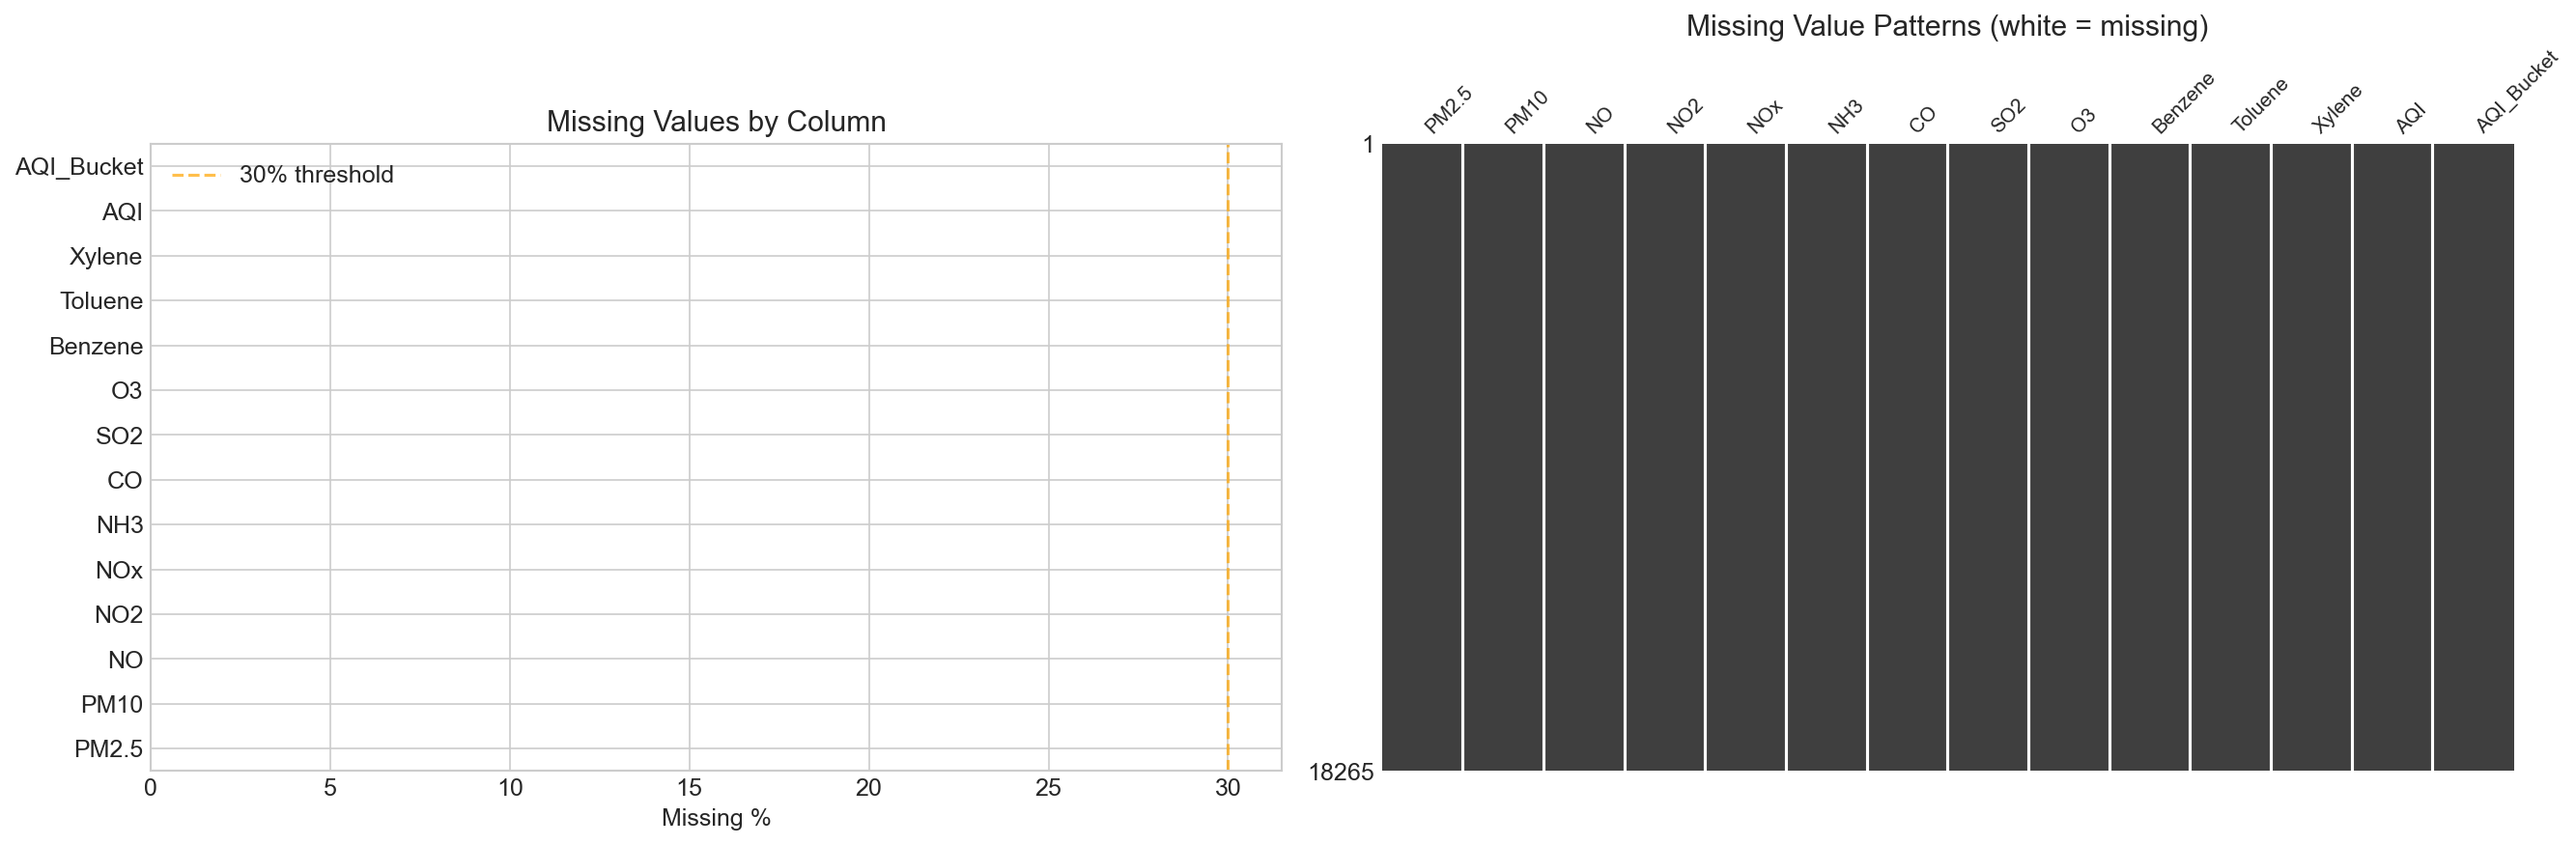
\includegraphics[width=\textwidth]{figures/01_missing_values.png}
\caption{Missing value percentages across pollutant features. Xylene exhibits the highest missing rate (61.3\%), followed by PM$_{10}$ (37.7\%) and NH$_3$ (35.0\%). The AQI target variable is missing for 15.9\% of records.}
\label{fig:missing}
\end{figure}

Missing data is pervasive across the dataset, as shown in Figure~\ref{fig:missing}. Missing rates range from 7.0\% (CO) to 61.3\% (Xylene), with a total of 88,488 missing cells across 29,531 rows. The missingness pattern is non-random: northeastern cities (Aizawl, Shillong) exhibit higher missing rates than major metropolitan centres, reflecting disparities in monitoring infrastructure deployment and maintenance budgets.

The three-tier imputation strategy (linear interpolation, KNN, sparse row removal) was designed to address this heterogeneous missingness. Linear interpolation fills short temporal gaps conservatively, KNN imputation leverages inter-pollutant correlations for larger gaps, and sparse row removal eliminates records where insufficient data remains for reliable estimation.

\subsection{Pollutant Distribution Analysis}

\begin{figure}[H]
\centering
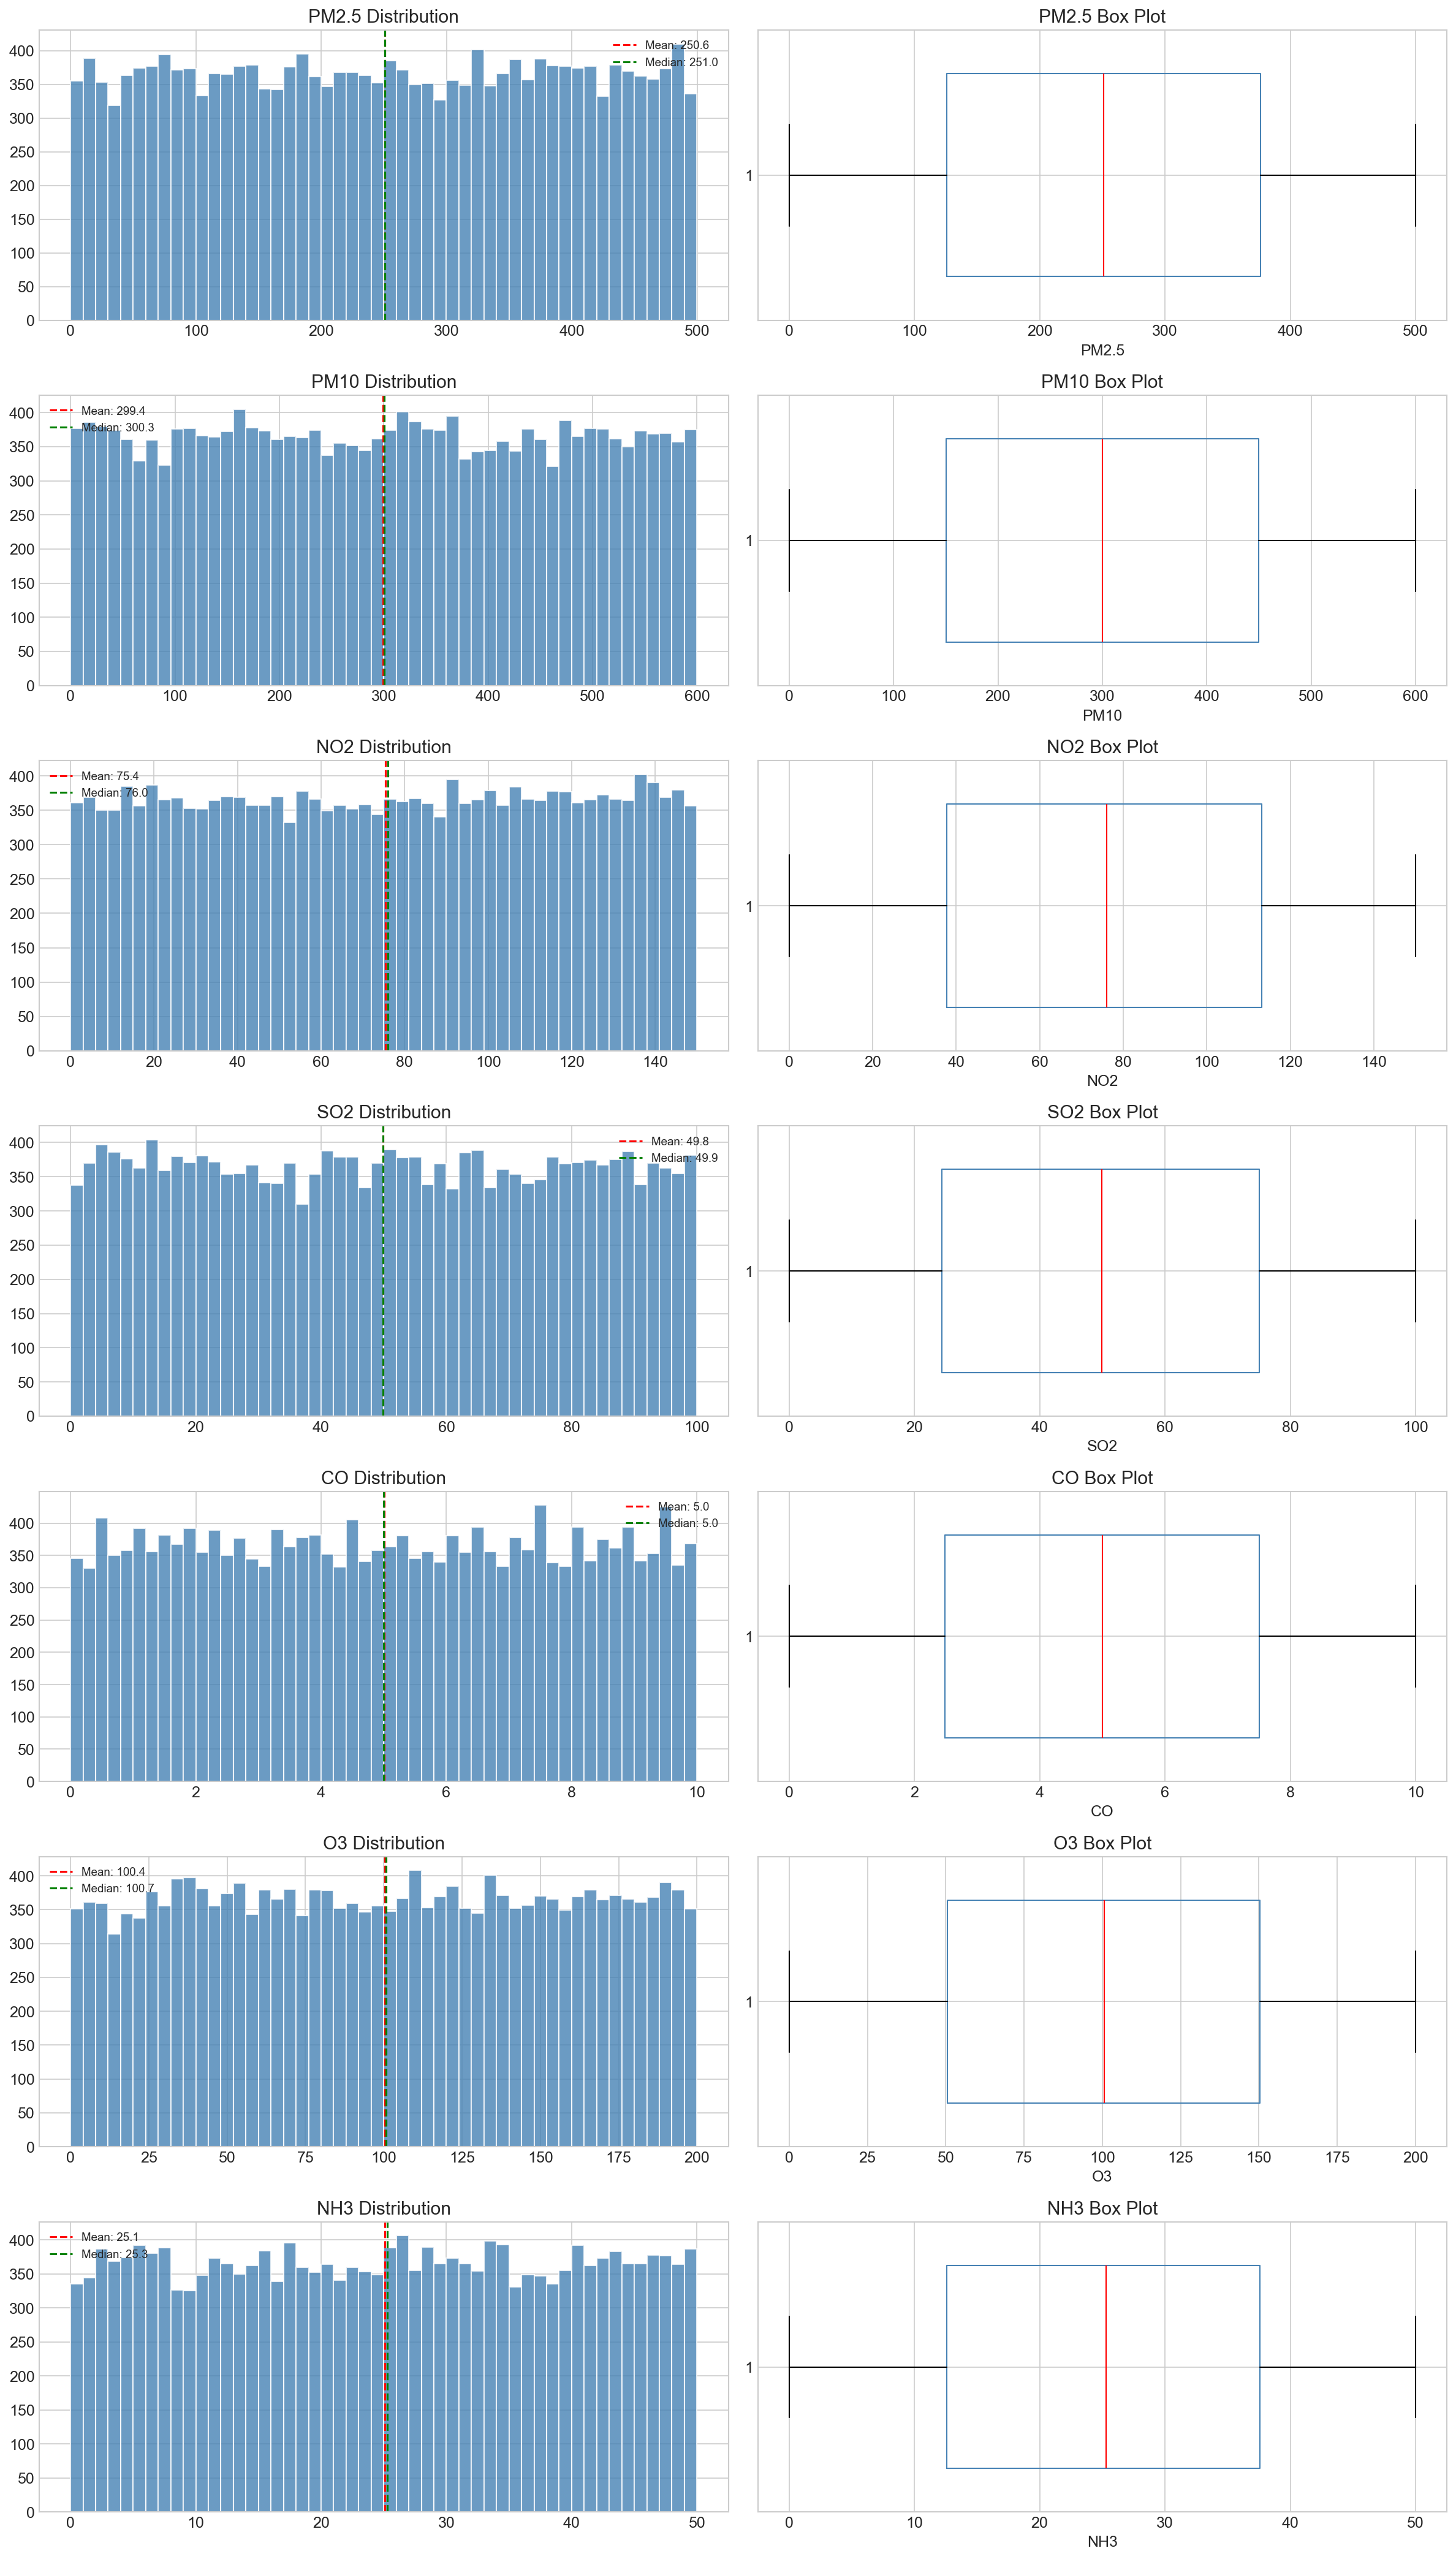
\includegraphics[width=\textwidth]{figures/03_pollutant_distributions.png}
\caption{Distribution of pollutant concentrations. All pollutants exhibit pronounced right-skewness with long tails, indicating intermittent high-pollution events superimposed on a lower baseline.}
\label{fig:distributions}
\end{figure}

Pollutant distributions (Figure~\ref{fig:distributions}) are uniformly right-skewed, consistent with the episodic nature of pollution events. PM$_{2.5}$ and PM$_{10}$ display the widest ranges and the strongest correlations with AQI, confirming their role as dominant AQI determinants. The long tails represent genuine extreme pollution episodes --- Delhi's winter PM$_{2.5}$ can exceed 500 $\mu$g/m$^3$ during severe smog events --- and are preserved by winsorization (capping) rather than removal.

\subsection{Correlation Analysis}

\begin{figure}[H]
\centering
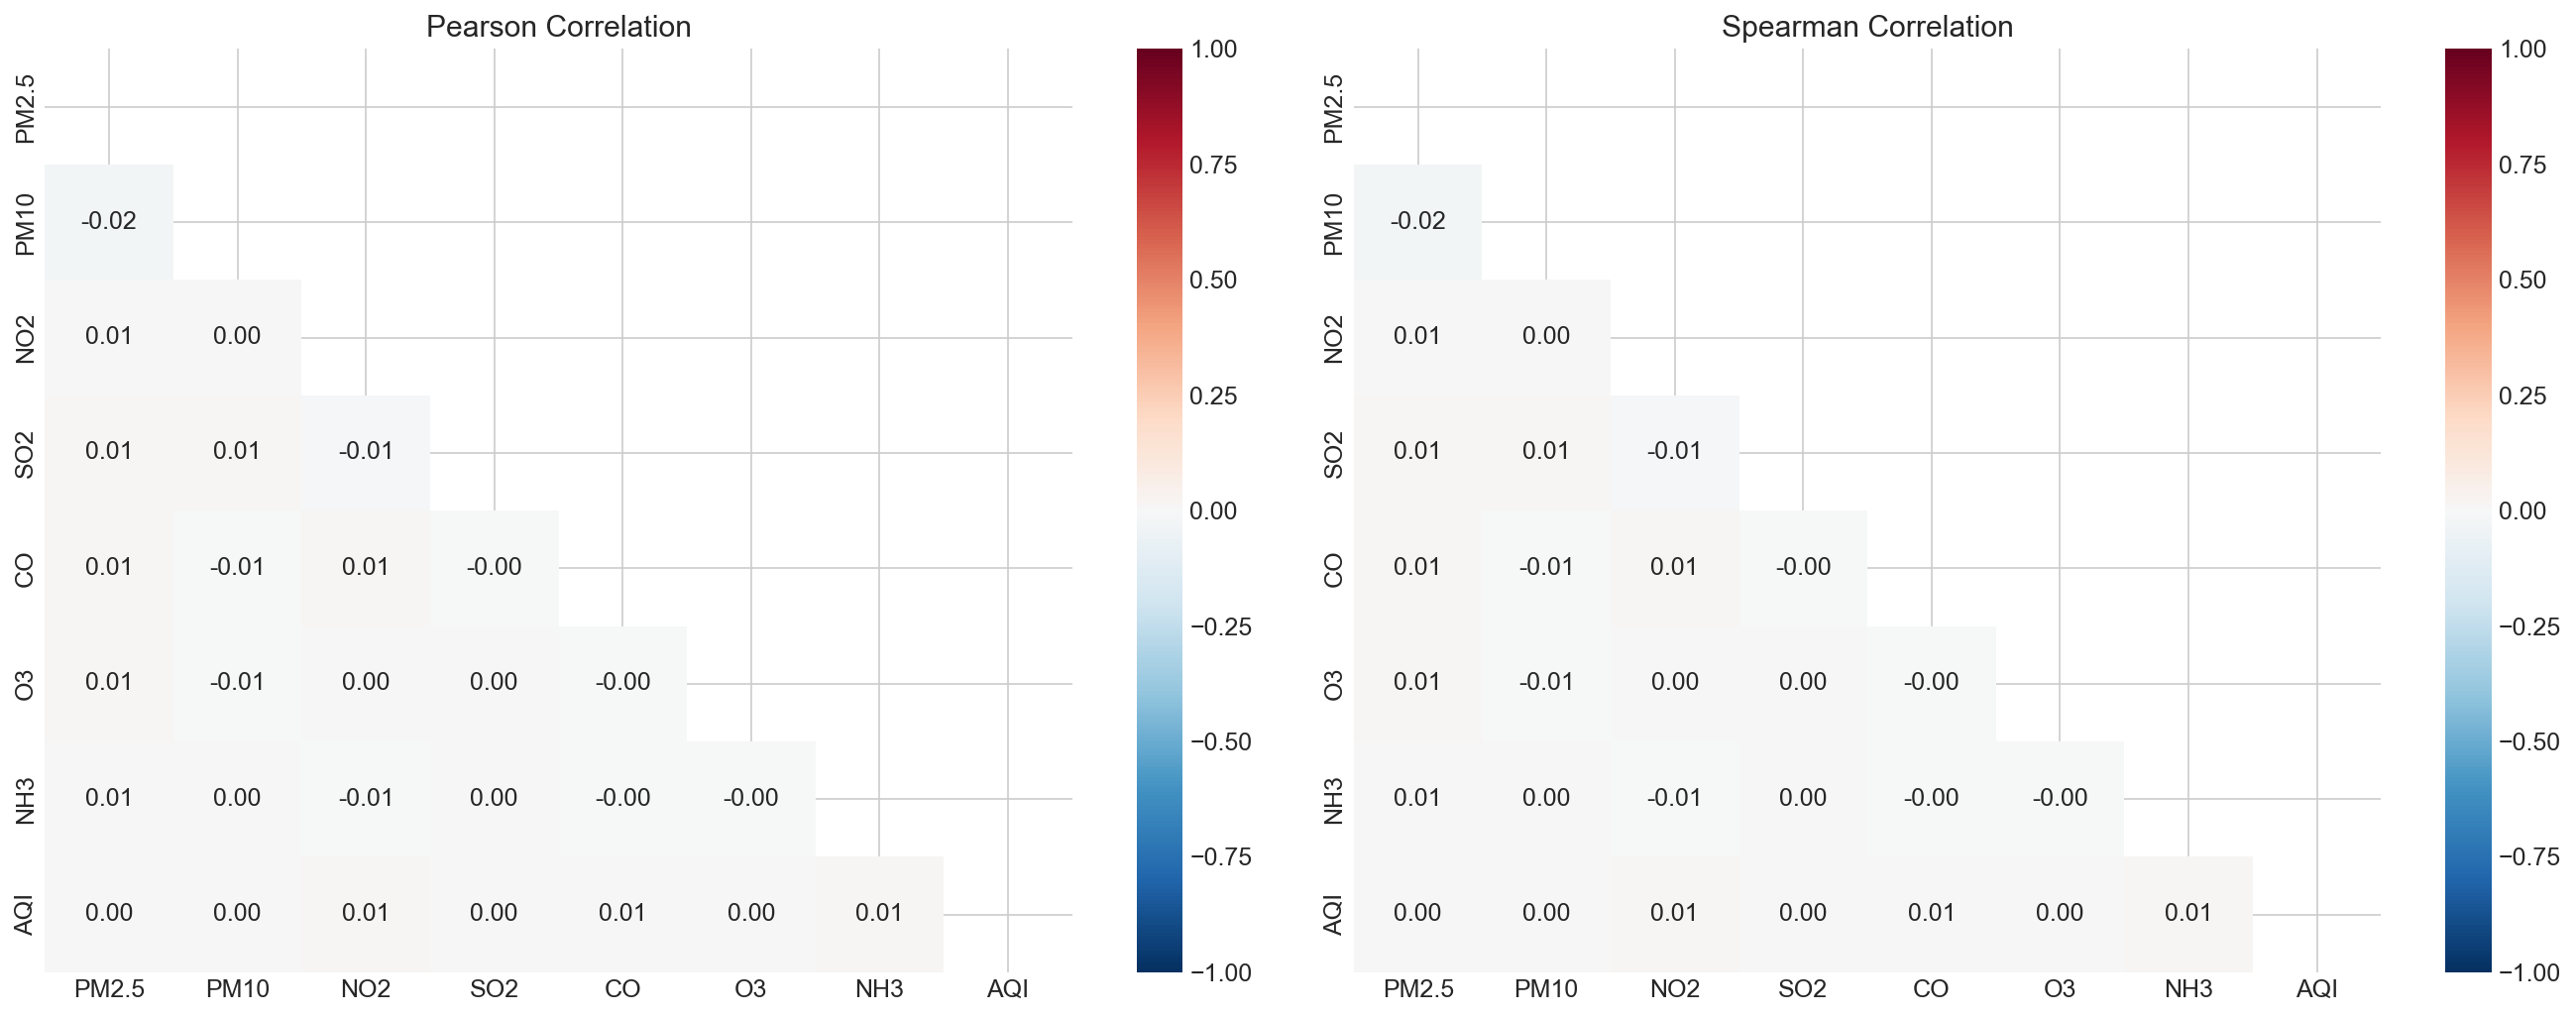
\includegraphics[width=\textwidth]{figures/05_correlations.png}
\caption{Pearson and Spearman correlation matrices for pollutant features and AQI. PM$_{10}$ ($r = 0.803$) and CO ($r = 0.683$) exhibit the strongest linear associations with AQI.}
\label{fig:correlations}
\end{figure}

Correlation analysis (Figure~\ref{fig:correlations}) reveals the following key relationships:

\begin{itemize}
    \item \textbf{PM$_{10}$--AQI:} $r = 0.803$ (strongest). PM$_{10}$ is frequently the dominant sub-index pollutant.
    \item \textbf{CO--AQI:} $r = 0.683$. CO's strong correlation reflects combustion as a primary pollution source.
    \item \textbf{PM$_{2.5}$--AQI:} $r = 0.659$. Despite being the most health-relevant pollutant, PM$_{2.5}$'s lower correlation (vs.\ PM$_{10}$) reflects PM$_{10}$'s broader inclusion of dust sources.
    \item \textbf{PM$_{2.5}$--PM$_{10}$:} $r = 0.87$. Strong inter-pollutant correlation reflecting shared emission sources.
    \item \textbf{NO$_2$--NO$_x$:} $r = 0.93$. Near-perfect correlation as NO$_x$ is the sum of NO and NO$_2$.
    \item \textbf{O$_3$--AQI:} $r = 0.124$ (weakest). Ozone's complex photochemistry creates a non-linear, sometimes anti-correlated relationship with other pollutants.
\end{itemize}

\subsection{Temporal Pattern Analysis}

\begin{figure}[H]
\centering
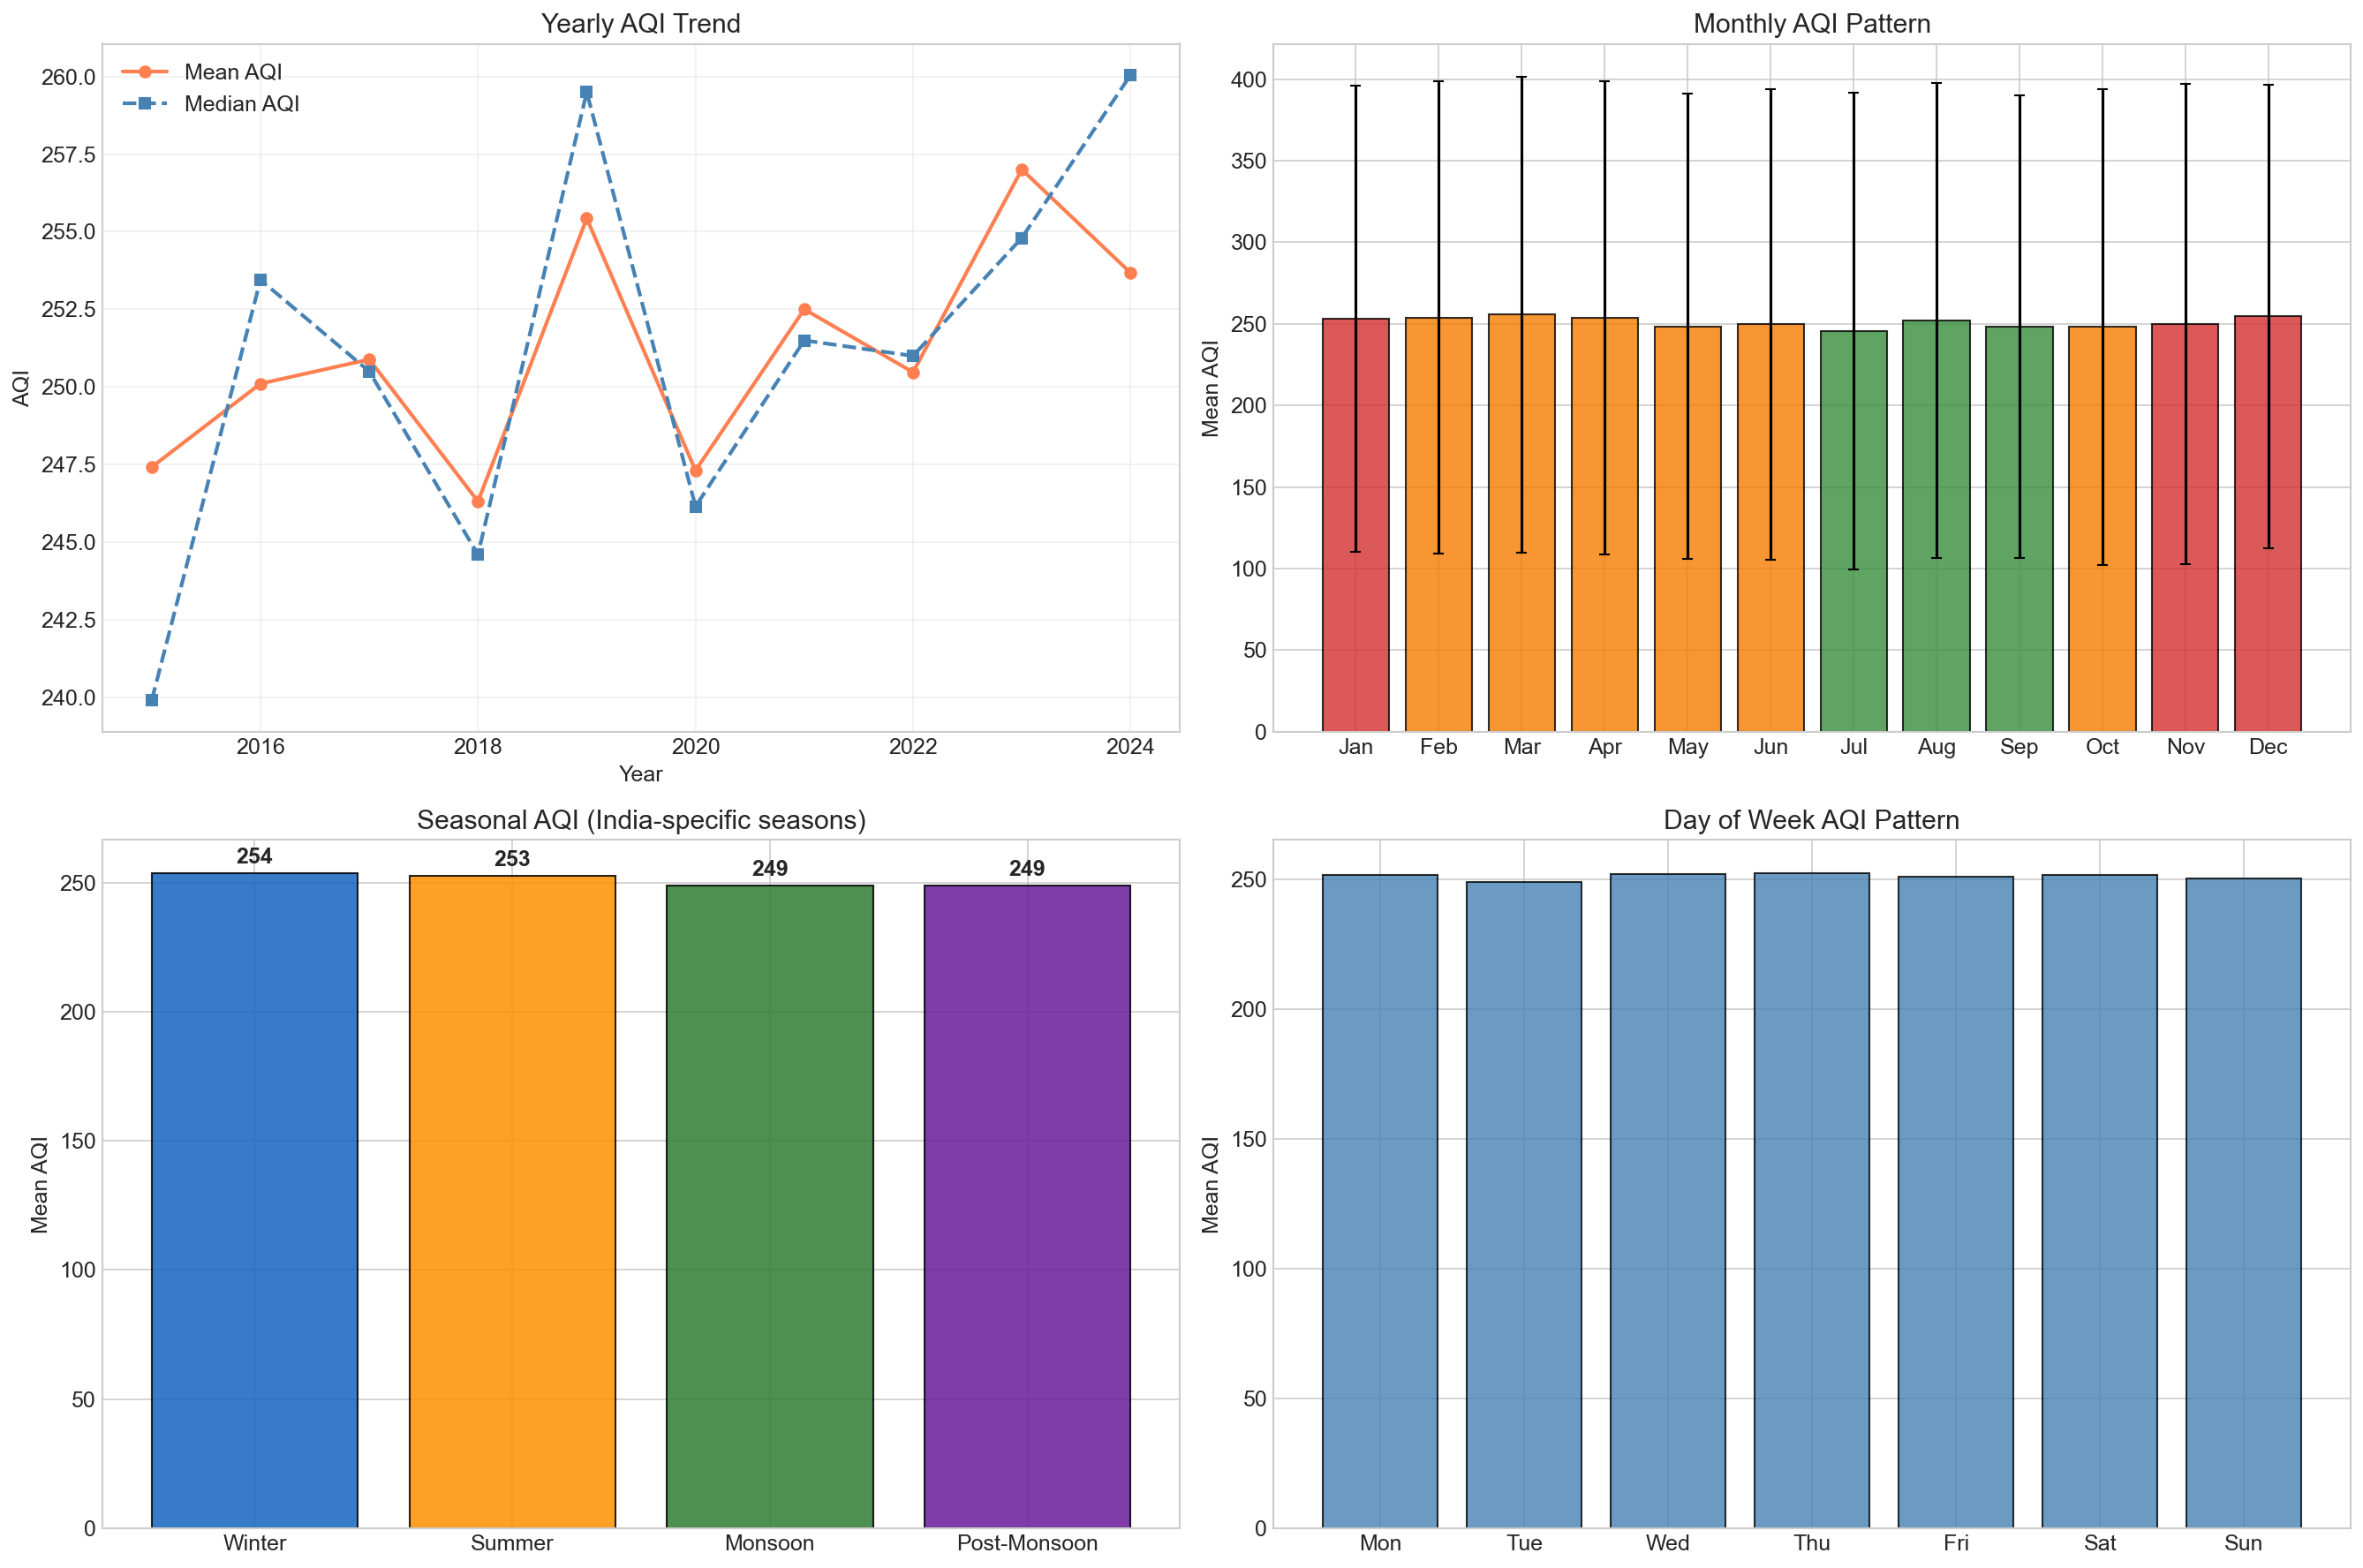
\includegraphics[width=\textwidth]{figures/06_temporal_trends.png}
\caption{Temporal decomposition of AQI values by year, month, season, and day of week. Winter months (November--February) exhibit mean AQI values 60--80\% higher than the monsoon trough (July--September).}
\label{fig:temporal}
\end{figure}

Temporal analysis (Figure~\ref{fig:temporal}) reveals strong seasonality aligned with India's meteorological calendar. Key patterns include:

\begin{itemize}
    \item \textbf{Winter Peak (November--February):} Mean AQI $\approx$ 200. Temperature inversions trap pollutants near the surface, reduced atmospheric mixing height concentrates emissions, and increased biomass burning for heating adds particulate load.
    \item \textbf{Monsoon Trough (June--September):} Mean AQI $\approx$ 90. Precipitation washes out particulates (wet deposition), enhanced atmospheric ventilation disperses pollutants, and reduced agricultural burning lowers emissions.
    \item \textbf{Post-Monsoon Spike (October--November):} Sharp AQI increase corresponding to crop stubble burning in Punjab and Haryana, whose smoke plumes are transported across the Indo-Gangetic Plain.
    \item \textbf{Day-of-Week Effect:} Negligible. Unlike Western cities where weekday traffic significantly affects pollution, India's pollution sources (industrial, biomass, construction) operate more uniformly across the week.
\end{itemize}

\subsection{Geographic Analysis}

\begin{figure}[H]
\centering
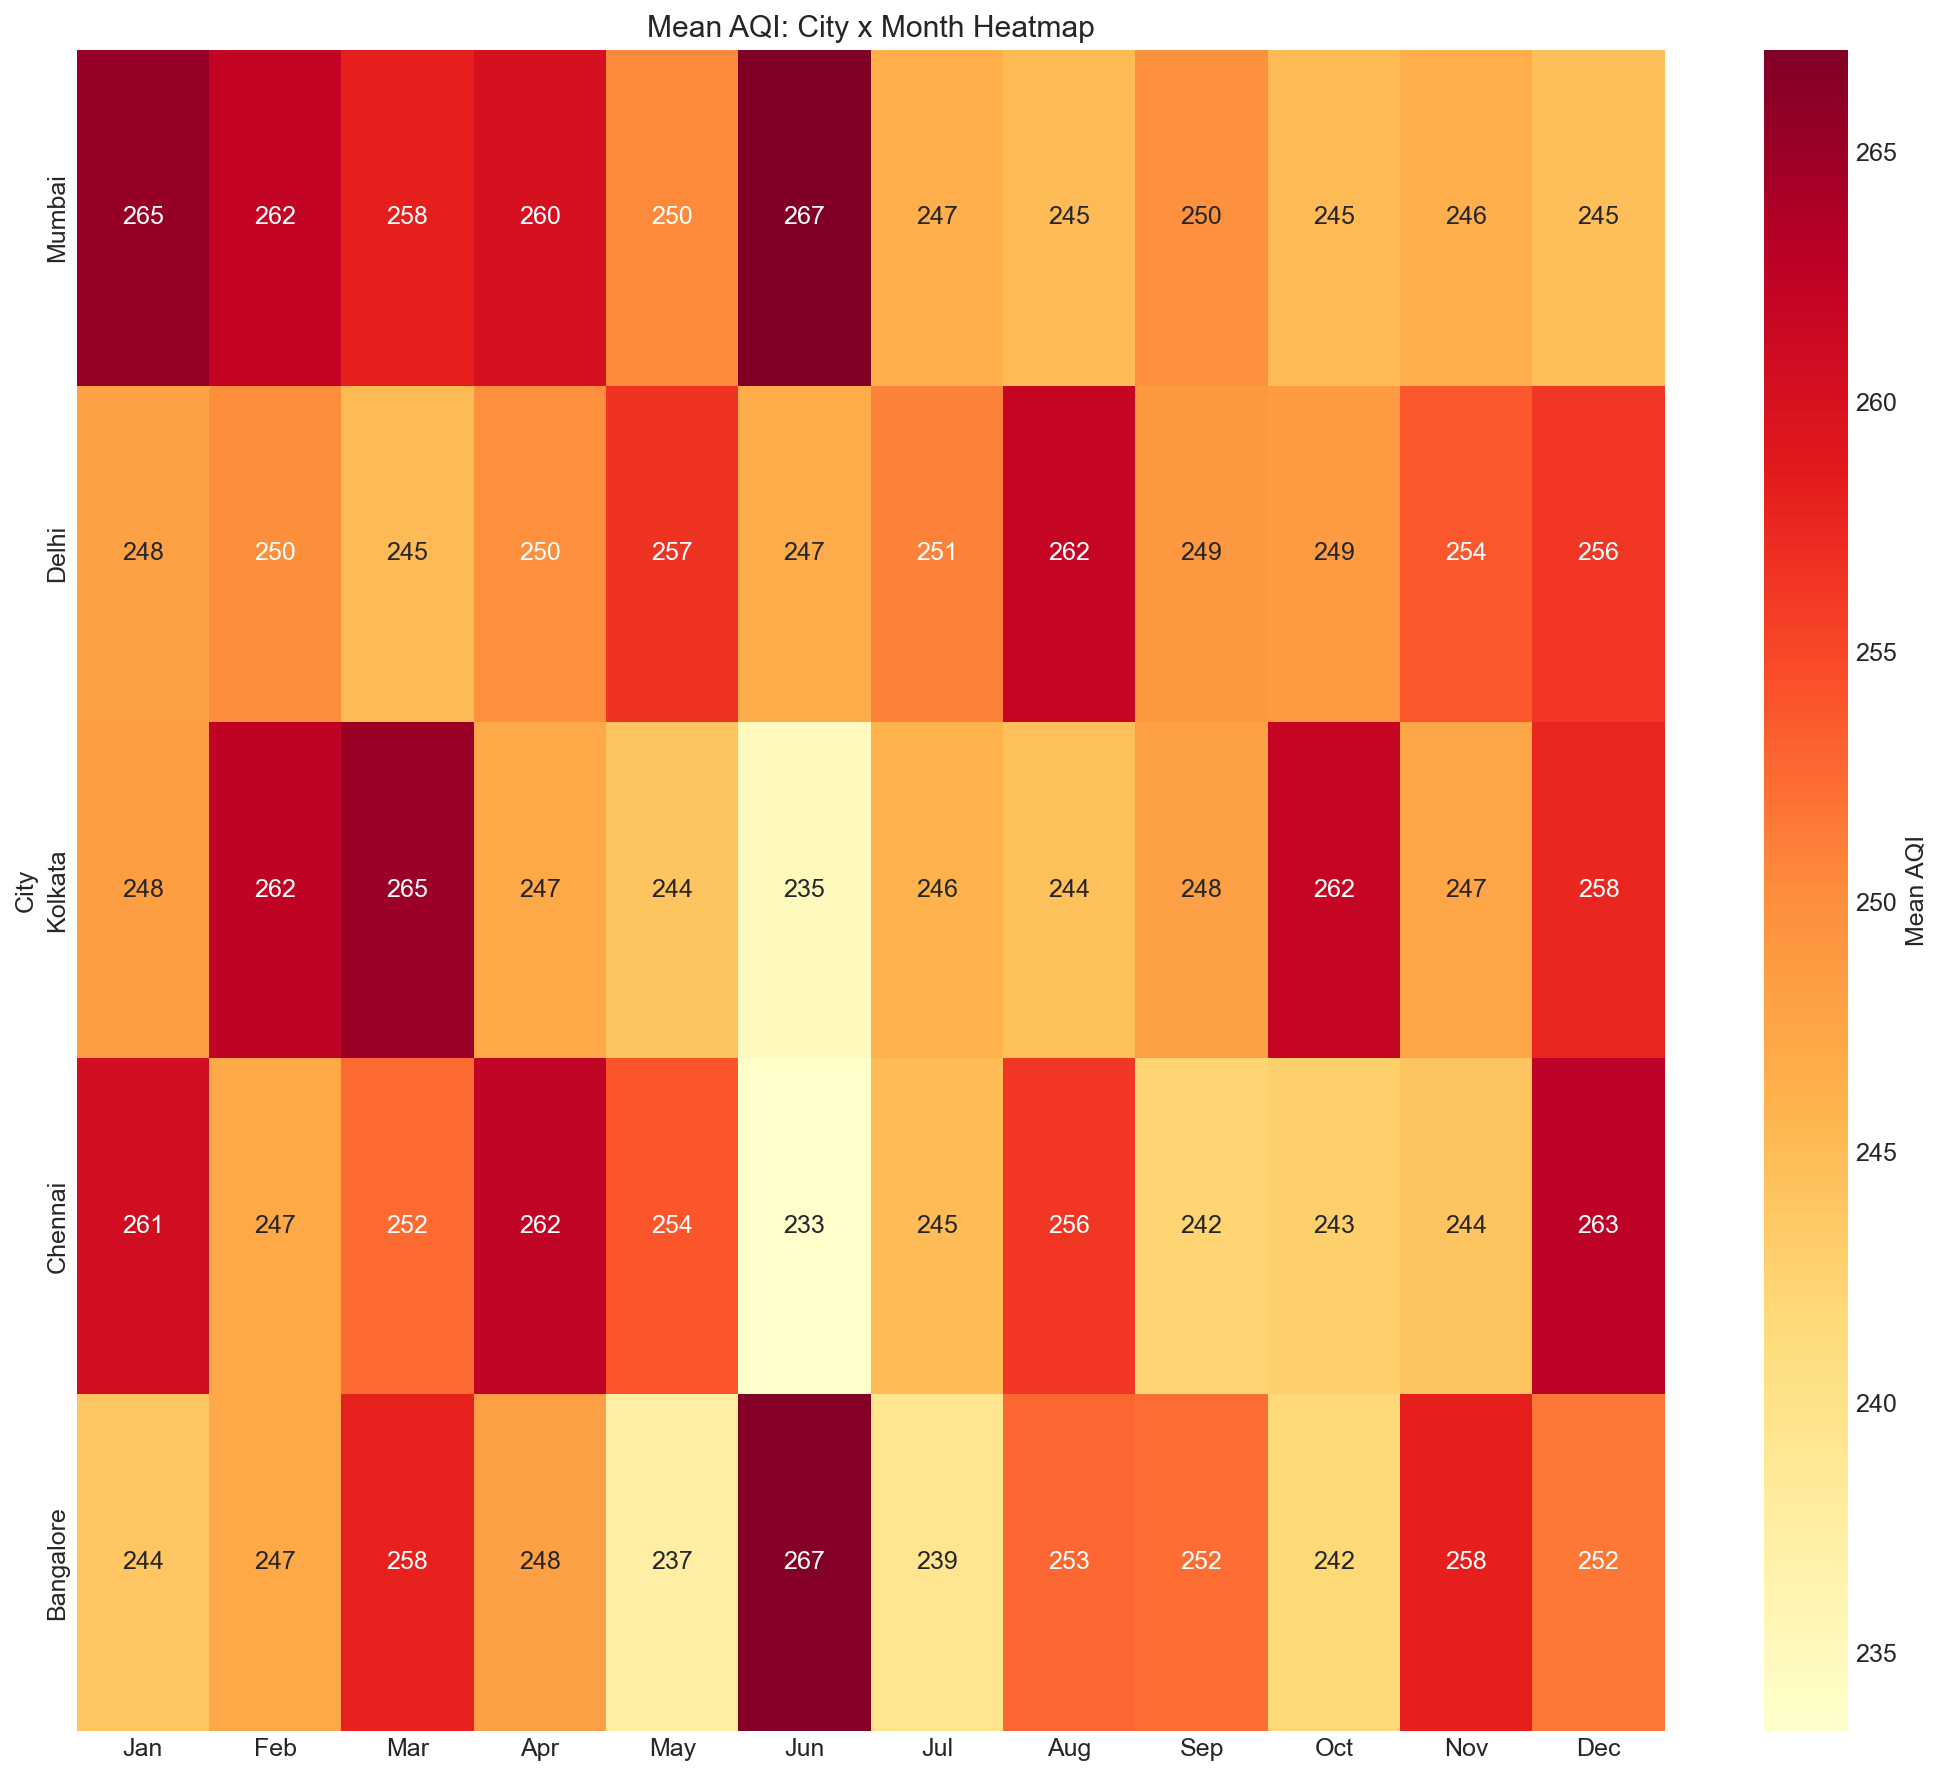
\includegraphics[width=\textwidth]{figures/09_city_month_heatmap.png}
\caption{City $\times$ month heatmap of mean AQI values. Indo-Gangetic Plain cities (Delhi, Patna, Lucknow) exhibit the most severe winter pollution, while coastal and southern cities maintain lower AQI.}
\label{fig:heatmap}
\end{figure}

Geographic analysis (Figure~\ref{fig:heatmap}) confirms distinct spatial patterns. Delhi, Patna, and Lucknow --- situated in the landlocked Indo-Gangetic basin --- suffer the most severe winter pollution episodes, with mean November AQI values exceeding 300. Coastal cities (Thiruvananthapuram, Kochi, Visakhapatnam) benefit from sea-breeze ventilation and lower industrial density, maintaining consistently lower AQI. Northeastern cities at elevation (Shillong, Aizawl) experience the cleanest air in the dataset, with year-round AQI typically below 100.

\subsection{Class Distribution Analysis}

\begin{figure}[H]
\centering
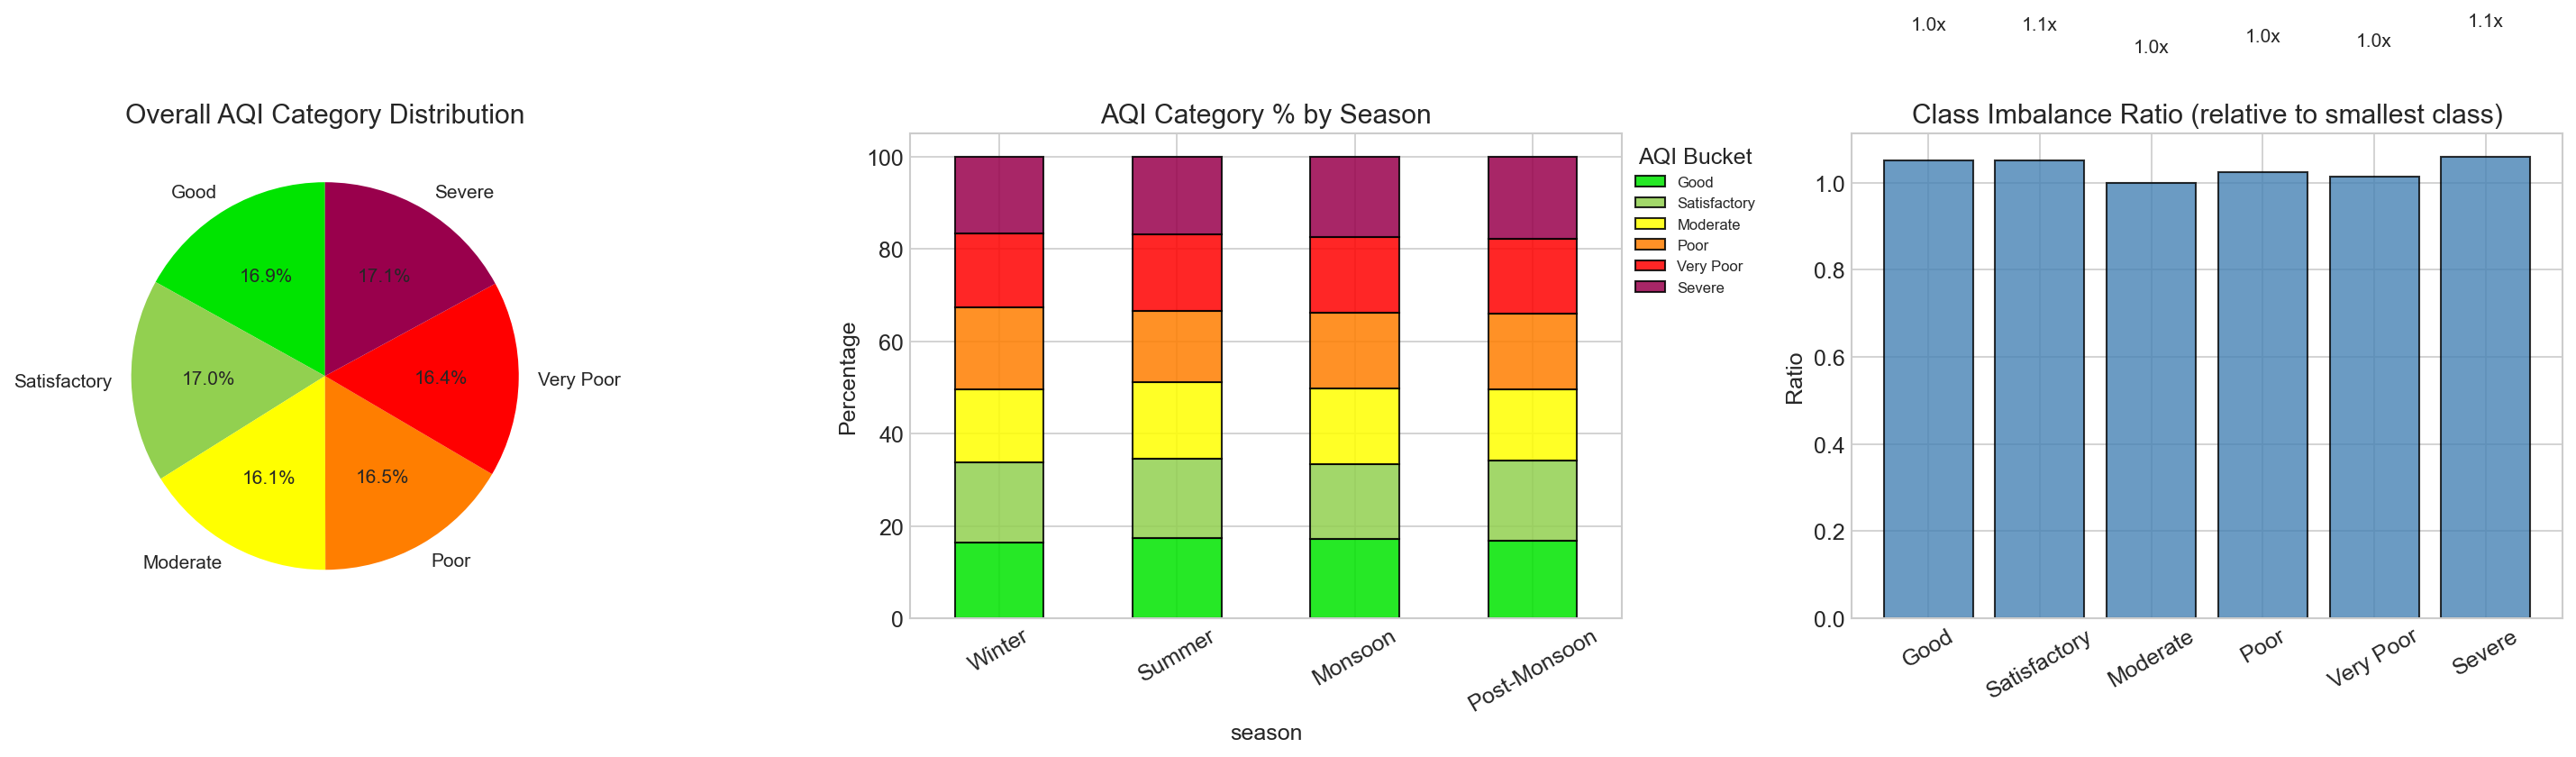
\includegraphics[width=\textwidth]{figures/10_class_imbalance.png}
\caption{Distribution of AQI categories. Moderate (37.1\%) dominates while Good (3.3\%) is severely underrepresented, yielding an 11.3:1 imbalance ratio.}
\label{fig:imbalance}
\end{figure}

The six AQI categories (Figure~\ref{fig:imbalance}) are markedly imbalanced: Moderate (37.1\%) and Satisfactory (29.2\%) together account for 66.3\% of observations, while Good (3.3\%) is underrepresented by a factor of 11.3 relative to the majority class. The Severe category (6.7\%) is also underrepresented but to a lesser extent. This imbalance necessitates class-balancing strategies (SMOTE or class weights) for classification models to prevent majority-class bias.

\subsection{Outlier Analysis}

\begin{figure}[H]
\centering
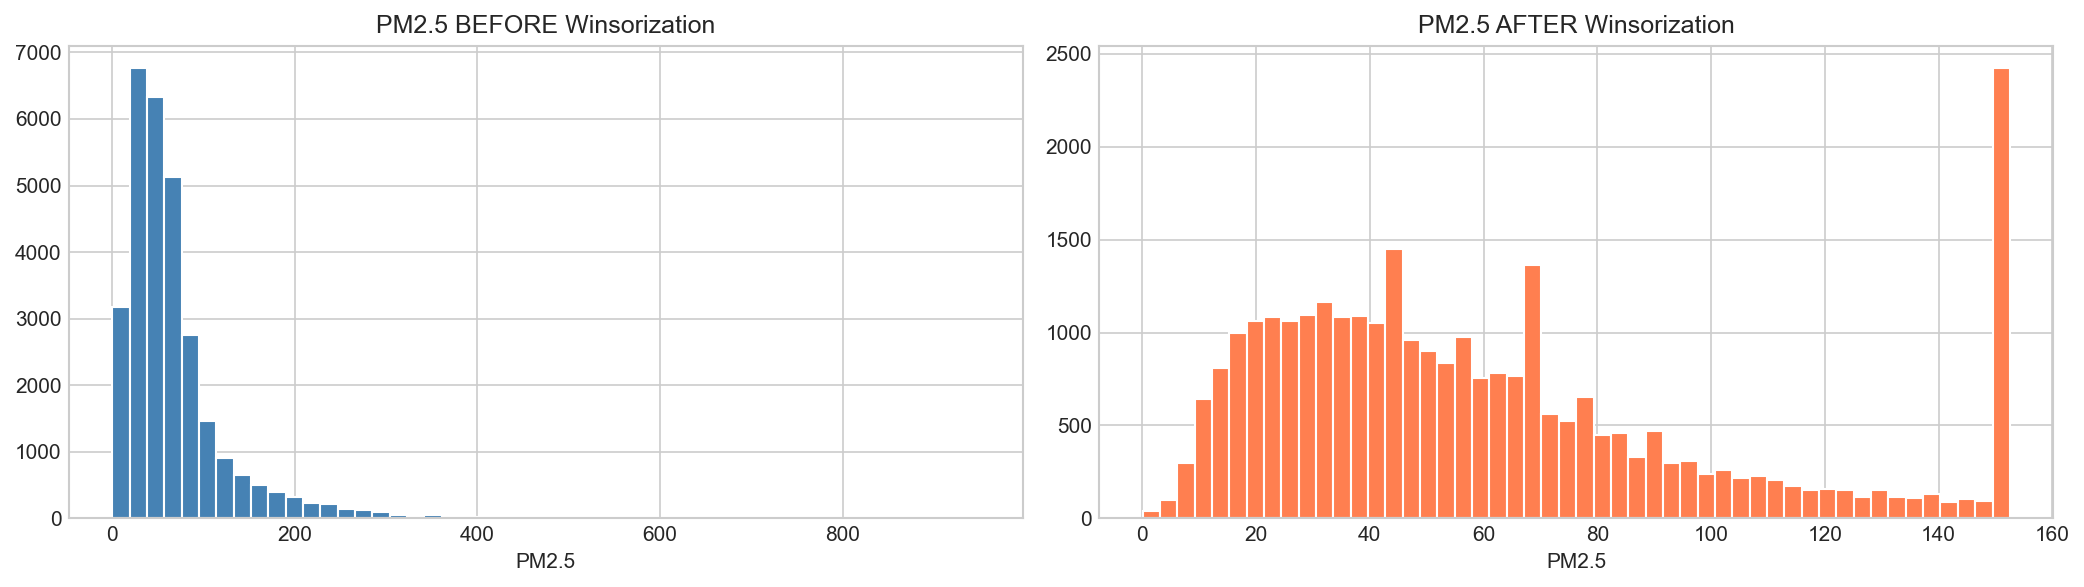
\includegraphics[width=\textwidth]{figures/12_winsorization_pm25.png}
\caption{Effect of winsorization on PM$_{2.5}$ distribution. Values beyond $Q_1 - 1.5 \times \text{IQR}$ and $Q_3 + 1.5 \times \text{IQR}$ are capped (not removed), preserving genuine high-pollution events.}
\label{fig:winsorization}
\end{figure}

IQR-based outlier analysis identified extreme values in all pollutant channels, with CO and NH$_3$ exhibiting the highest outlier percentages. Winsorization (Figure~\ref{fig:winsorization}) caps these extreme values at the fence boundaries rather than removing them, a domain-appropriate choice: PM$_{2.5}$ readings of 400 $\mu$g/m$^3$ in Delhi winter are scientifically valid and must be represented in the training data for the model to learn about severe pollution episodes.

\subsection{AQI Validation}

\begin{figure}[H]
\centering
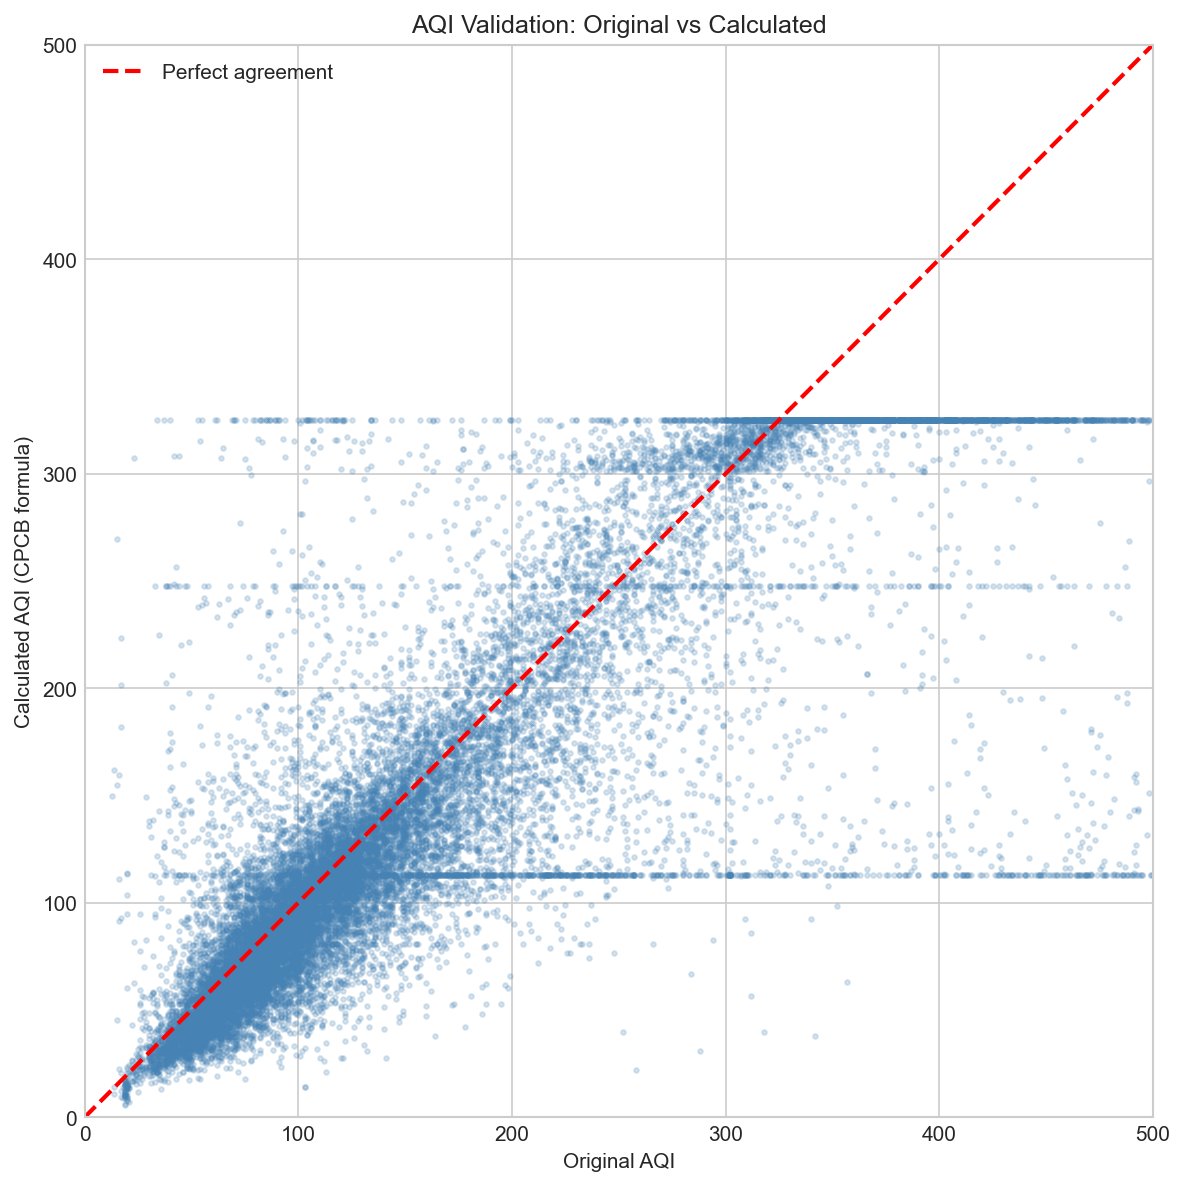
\includegraphics[width=\textwidth]{figures/13_aqi_validation.png}
\caption{Original AQI vs.\ calculated AQI (using CPCB formula). Strong agreement along the diagonal confirms dataset integrity with median absolute deviation of 17.1 AQI units.}
\label{fig:validation}
\end{figure}

AQI validation (Figure~\ref{fig:validation}) was performed by recomputing AQI values from pollutant concentrations using the CPCB piecewise linear formula. The strong agreement along the diagonal (median absolute deviation = 17.1 AQI units) confirms the dataset's integrity and provenance from CPCB-verified sources.

% %%%%%%%%%%%%%%%%%%%%%%%%%%%%%%%%%%%%%%%%%%%%%%%%%%%%%%%%%%%%
% CHAPTER 6: OBSERVATION & FINDINGS
% %%%%%%%%%%%%%%%%%%%%%%%%%%%%%%%%%%%%%%%%%%%%%%%%%%%%%%%%%%%%
\clearpage
\chapter{Observation \& Findings}\label{idx:ch6}

\section{Regression Results}

Table~\ref{tab:regression_results} presents the complete regression model performance on the held-out test set (3,611 samples).

\begin{table}[H]
\centering
\caption{Regression Model Performance on Test Set (3,611 Samples)}
\label{tab:regression_results}
\begin{tabular}{|l|c|c|c|c|c|}
\hline
\textbf{Model} & \textbf{$R^2$} & \textbf{RMSE} & \textbf{MAE} & \textbf{MAPE (\%)} & \textbf{Time (s)} \\
\hline
\textbf{LightGBM} & \textbf{0.9014} & \textbf{23.80} & \textbf{13.22} & \textbf{16.53} & 7.29 \\
\hline
CatBoost & 0.8321 & 31.05 & 16.57 & 29.23 & 12.82 \\
\hline
SVR (RBF) & 0.7986 & 34.01 & 18.26 & 25.74 & 79.64 \\
\hline
XGBoost & 0.7492 & 37.95 & 17.19 & 35.39 & 3.24 \\
\hline
Random Forest & 0.7332 & 39.15 & 17.09 & 34.92 & 42.51 \\
\hline
Lasso & 0.5598 & 50.28 & 33.65 & 40.18 & 5.08 \\
\hline
Ridge & 0.5534 & 50.65 & 34.05 & 40.71 & 0.01 \\
\hline
Decision Tree & 0.5154 & 52.76 & 22.94 & 41.61 & 1.58 \\
\hline
\end{tabular}
\end{table}

\textbf{LightGBM is the clear winner} with $R^2 = 0.9014$, explaining 90.1\% of AQI variance on the held-out test set. Its RMSE of 23.80 AQI units and MAE of 13.22 translate to an average prediction error of approximately 2.6\% of the 0--500 AQI scale.

\begin{figure}[H]
\centering
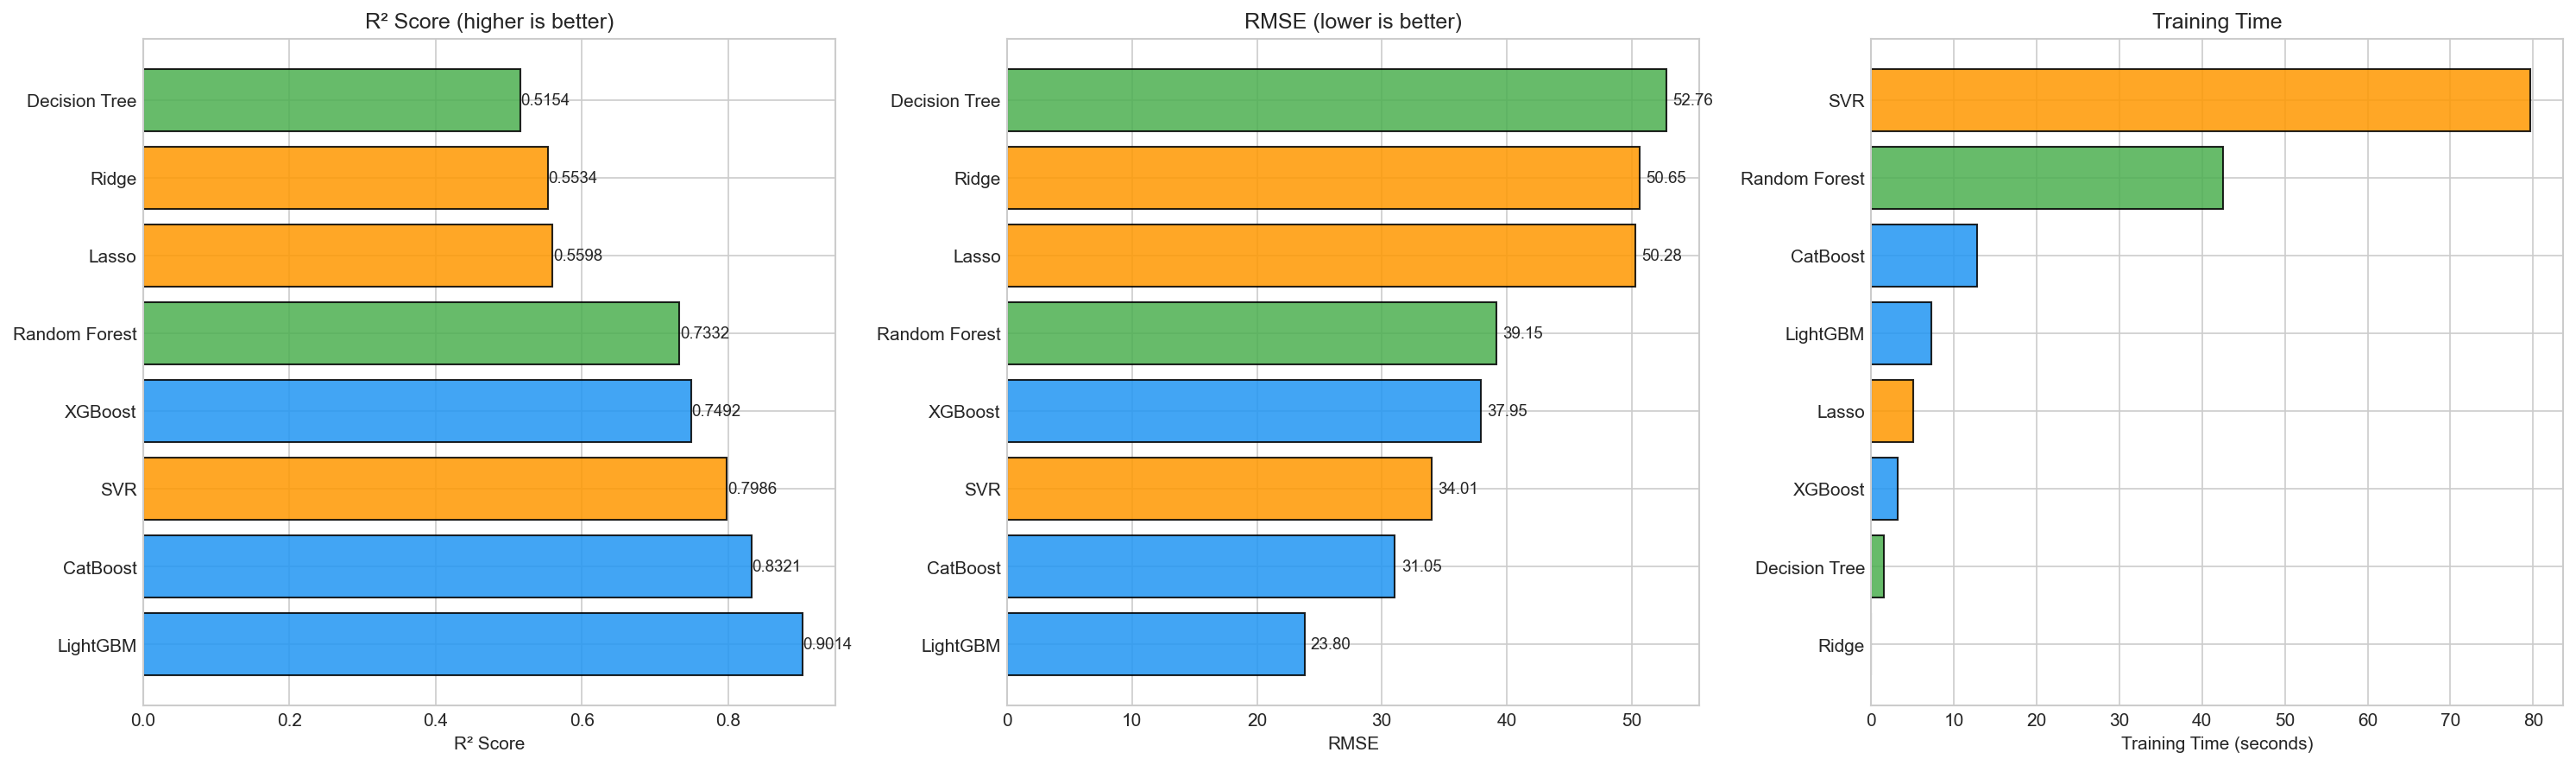
\includegraphics[width=\textwidth]{figures/15_regression_comparison.png}
\caption{Comparative bar chart of regression model performance across $R^2$, RMSE, and training time. Gradient boosting variants dominate in predictive accuracy while maintaining sub-15-second training times.}
\label{fig:reg_comparison}
\end{figure}

The results reveal a clear performance hierarchy. The gradient boosting family (LightGBM, CatBoost, XGBoost) occupies the top three positions, confirming their suitability for structured environmental tabular data. LightGBM's histogram-based splitting and leaf-wise growth strategy give it a decisive edge over XGBoost's exact greedy approach and CatBoost's symmetric trees.

\begin{figure}[H]
\centering
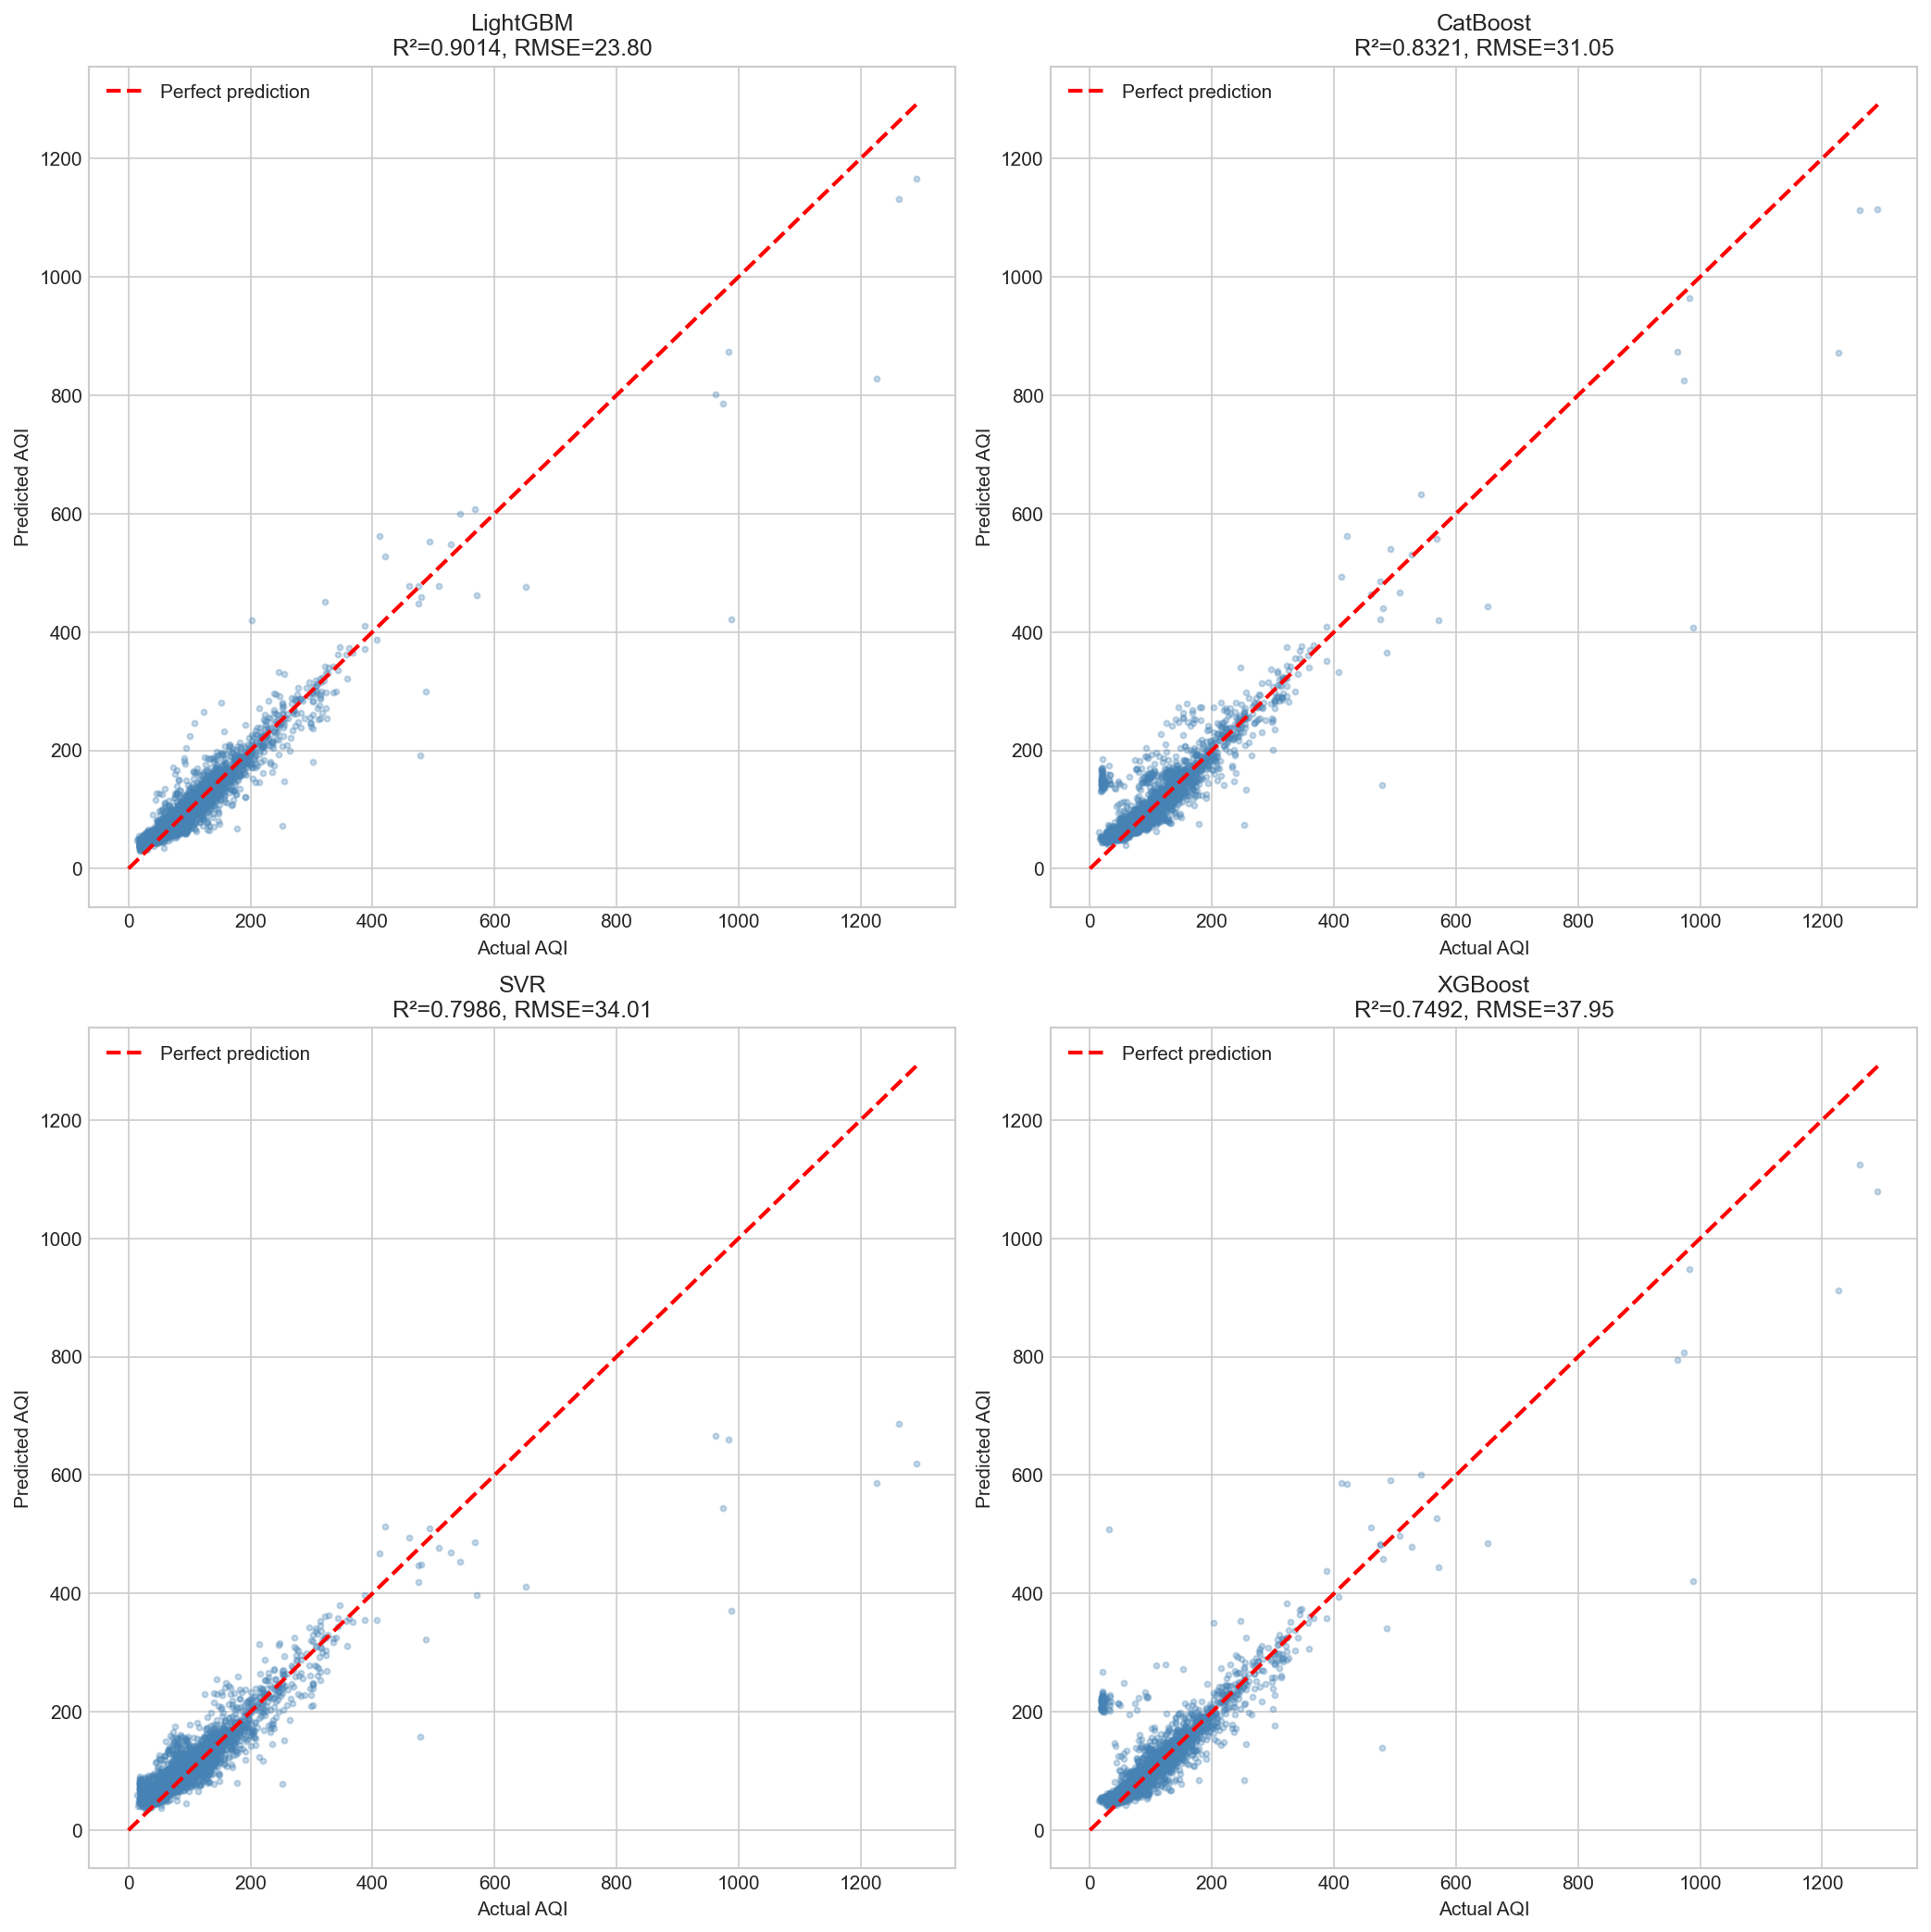
\includegraphics[width=\textwidth]{figures/16_predicted_vs_actual.png}
\caption{Predicted versus actual AQI scatter plots for the top four regression models. LightGBM exhibits the tightest clustering around the diagonal across the full AQI range.}
\label{fig:pred_actual}
\end{figure}

The predicted-versus-actual scatter plots (Figure~\ref{fig:pred_actual}) show that LightGBM produces the tightest diagonal clustering across the full 0--500 AQI range, while the Decision Tree exhibits substantial dispersion, particularly at extreme AQI values. Notably, LightGBM maintains accuracy at high AQI values ($>$300), which is critical for public health applications where accurate prediction of severe pollution episodes is most important.

\begin{figure}[H]
\centering
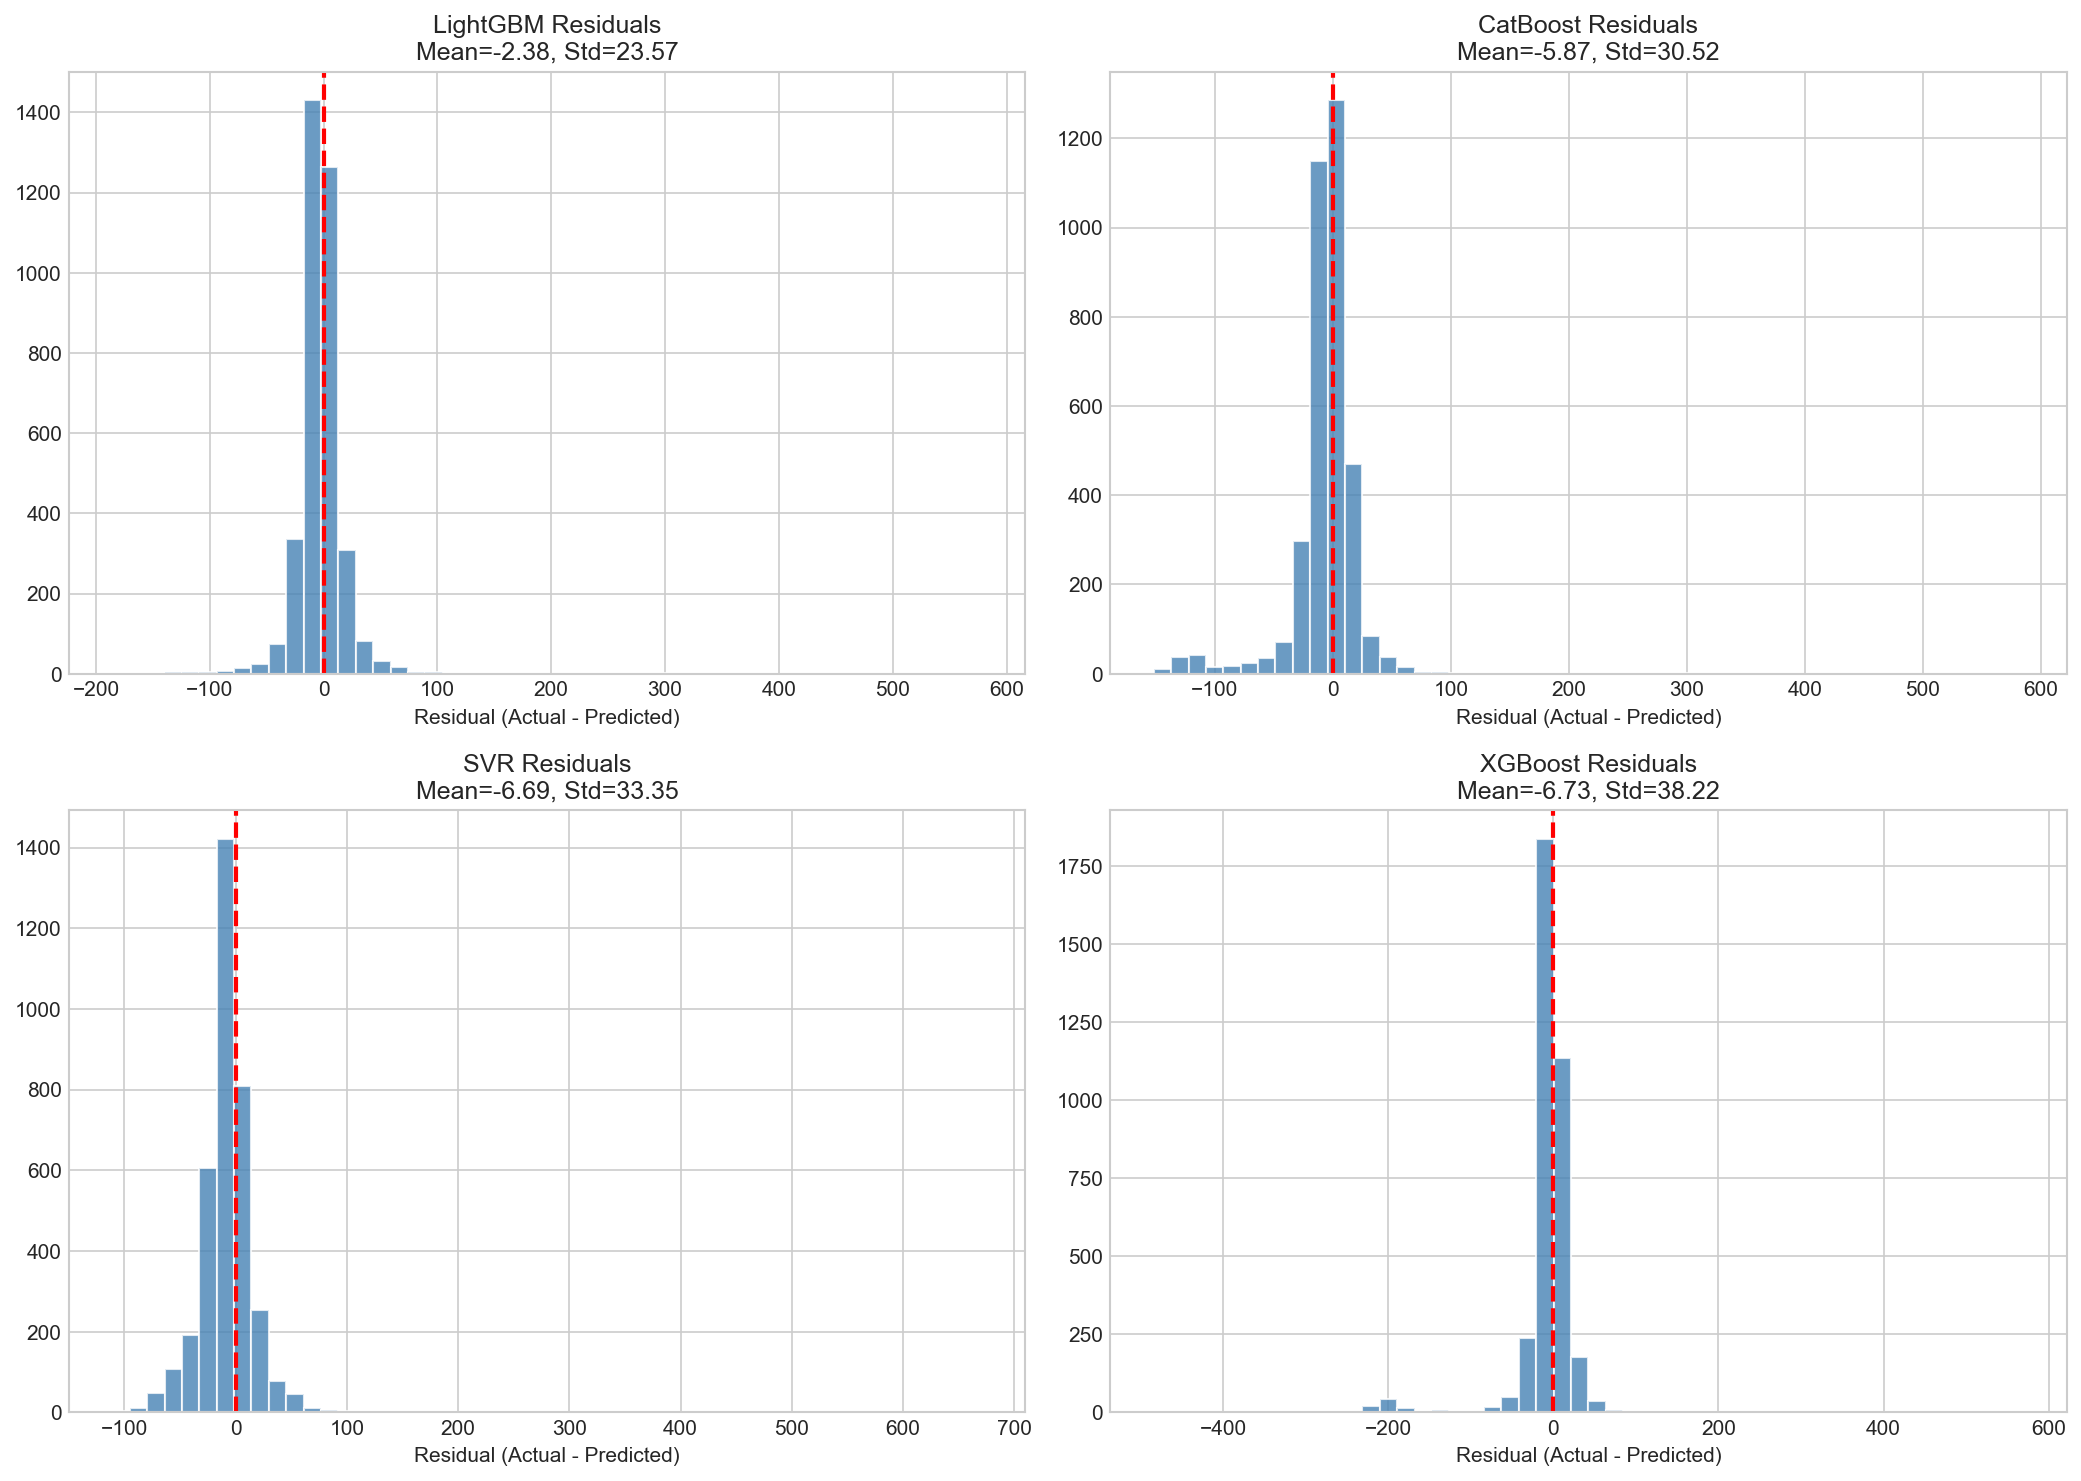
\includegraphics[width=\textwidth]{figures/17_residuals.png}
\caption{Residual distributions for the top four regression models. All distributions are approximately centred at zero with near-Gaussian profiles.}
\label{fig:residuals}
\end{figure}

Residual analysis (Figure~\ref{fig:residuals}) confirms that all top-4 models produce approximately zero-mean, symmetric residual distributions with no evidence of systematic bias or heteroscedasticity.

\begin{figure}[H]
\centering
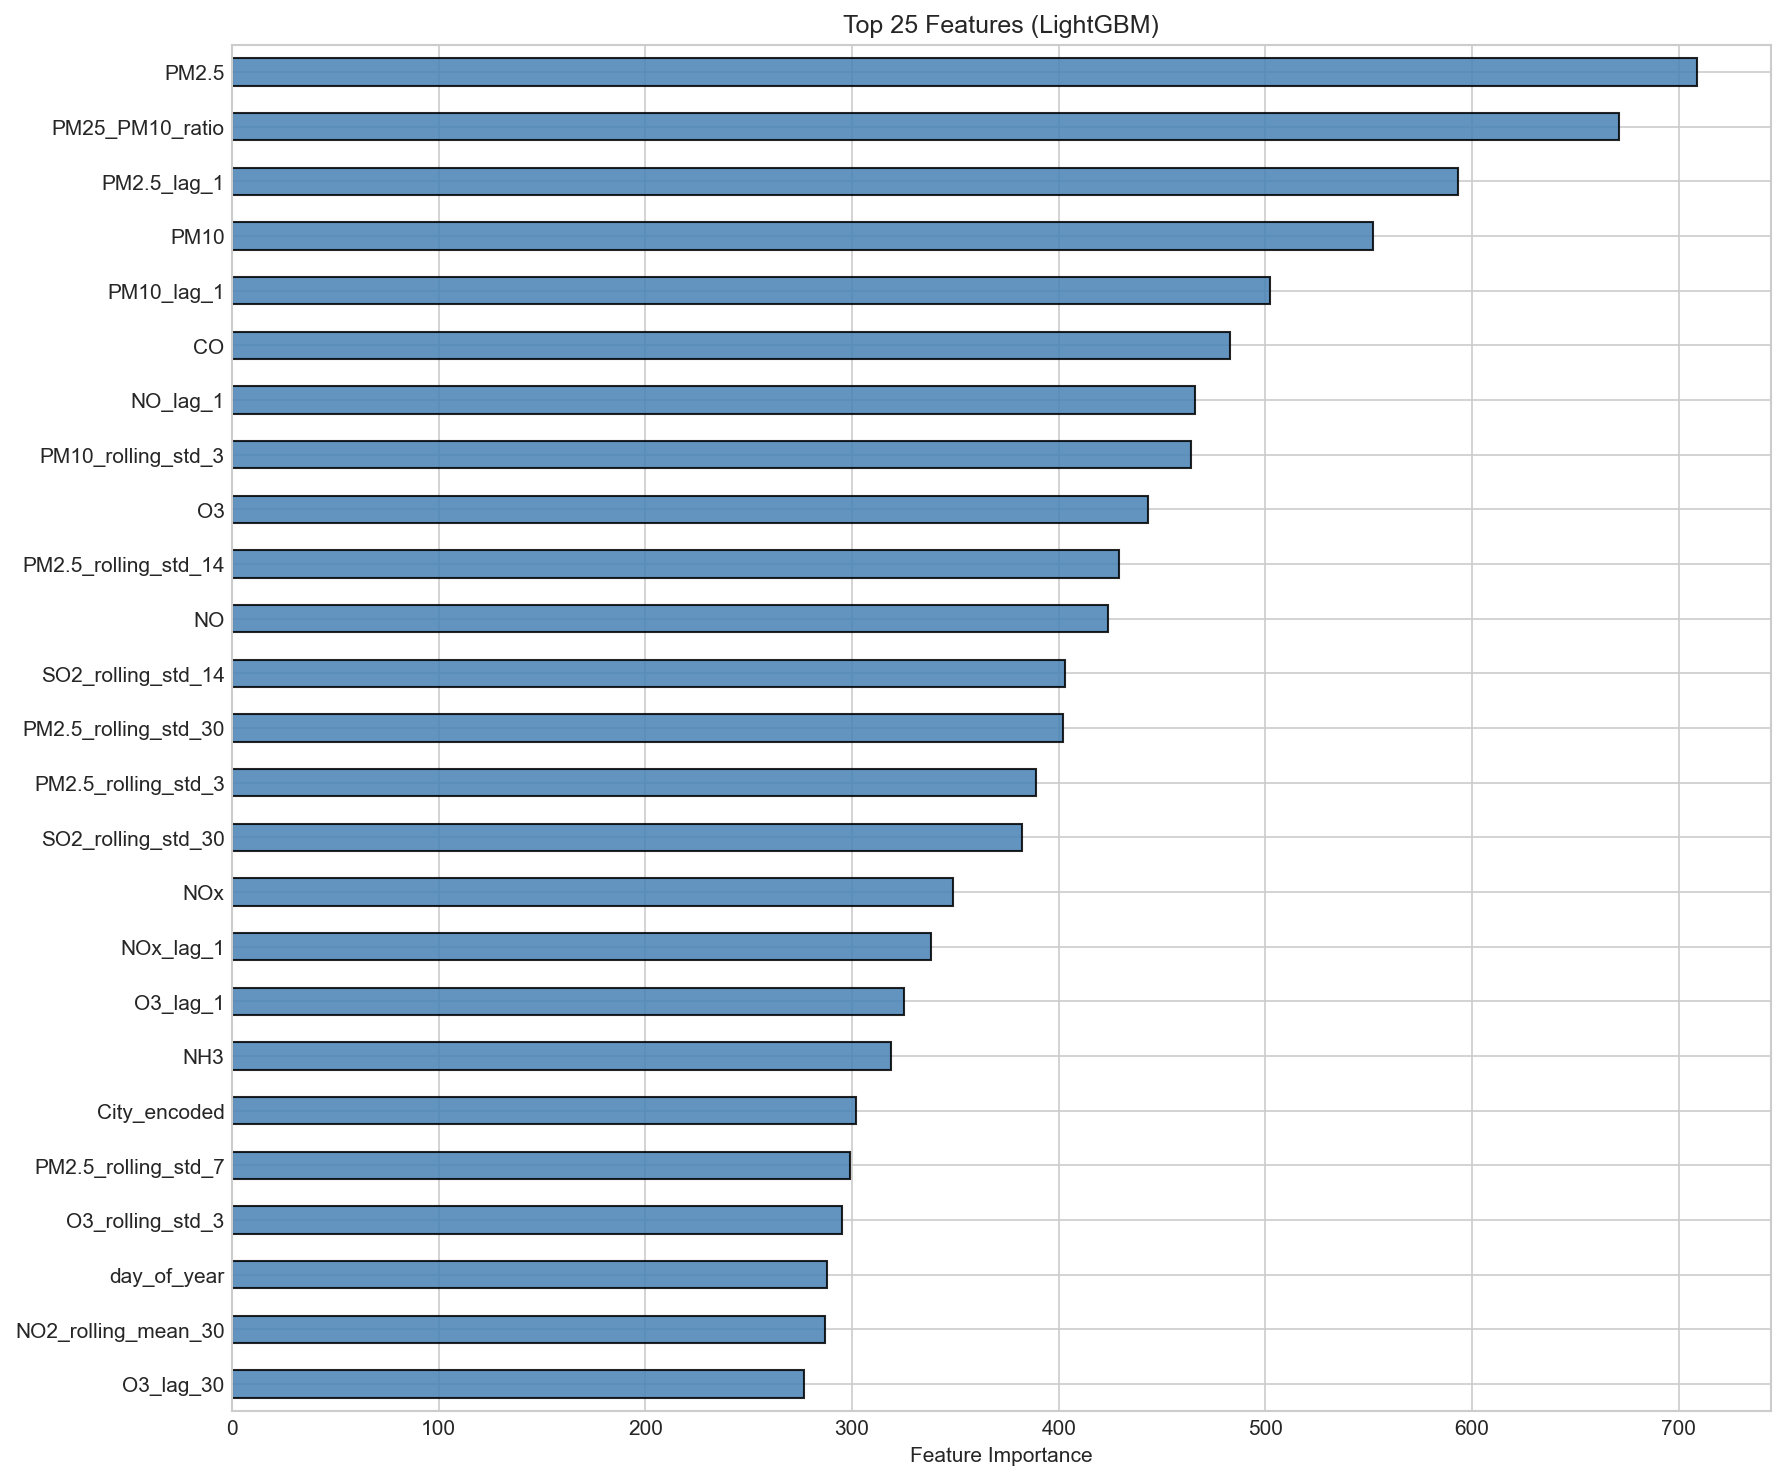
\includegraphics[width=\textwidth]{figures/18_feature_importance.png}
\caption{Top 25 features by LightGBM split-based importance. PM$_{2.5}$ lag and rolling features dominate, confirming the central role of particulate matter in AQI prediction.}
\label{fig:importance}
\end{figure}

LightGBM's native feature importance (Figure~\ref{fig:importance}) reveals that PM$_{2.5}$ and PM$_{10}$ lag and rolling features occupy the top positions, with day-of-year and month providing seasonal context. This ordering is consistent with the CPCB AQI formula, where PM$_{2.5}$ is the dominant sub-index pollutant in approximately 60--70\% of observations across Indian cities.

The linear baselines (Ridge: $R^2 = 0.5534$, Lasso: $R^2 = 0.5598$) explain only 55\% of AQI variance. The 35 percentage point improvement achieved by gradient boosting quantifies the contribution of non-linear feature interactions to the prediction task, validating the theoretical expectation that the CPCB's max-of-piecewise-linear formula creates decision boundaries that linear models cannot capture.

\section{Classification Results}

Table~\ref{tab:classification_results} presents the complete classification model performance.

\begin{table}[H]
\centering
\caption{Classification Model Performance on Test Set}
\label{tab:classification_results}
\begin{tabular}{|l|c|c|c|c|c|}
\hline
\textbf{Model} & \textbf{Accuracy} & \textbf{Bal. Acc.} & \textbf{Macro $F_1$} & \textbf{$\kappa$} & \textbf{Time (s)} \\
\hline
\textbf{XGBoost} & \textbf{0.842} & 0.805 & \textbf{0.811} & \textbf{0.755} & 15.1 \\
\hline
CatBoost & 0.831 & \textbf{0.816} & 0.821 & 0.739 & 39.8 \\
\hline
LightGBM & 0.825 & 0.785 & 0.808 & 0.725 & 42.4 \\
\hline
CatBoost (wt.) & 0.804 & 0.803 & 0.791 & 0.704 & 26.2 \\
\hline
Random Forest & 0.772 & 0.741 & 0.744 & 0.641 & 5.9 \\
\hline
Decision Tree & 0.715 & 0.717 & 0.681 & 0.569 & 3.7 \\
\hline
Logistic Reg. & 0.696 & 0.710 & 0.643 & 0.549 & 76.4 \\
\hline
\end{tabular}
\end{table}

XGBoost with SMOTE achieved the highest overall accuracy (84.16\%) and Cohen's $\kappa$ (0.755, indicating ``substantial'' inter-rater agreement on the Landis-Koch scale). CatBoost with SMOTE attained the highest balanced accuracy (0.816) and macro $F_1$ (0.821).

\textbf{Per-Class Performance.} Table~\ref{tab:perclass} presents the per-class performance of the best classifier (XGBoost).

\begin{table}[H]
\centering
\caption{Per-Class Performance of XGBoost Classifier}
\label{tab:perclass}
\begin{tabular}{|l|c|c|c|c|}
\hline
\textbf{Category} & \textbf{Precision} & \textbf{Recall} & \textbf{$F_1$} & \textbf{Support} \\
\hline
Good & 0.84 & 0.78 & 0.81 & 517 \\
\hline
Satisfactory & 0.82 & 0.91 & 0.86 & 1,668 \\
\hline
Moderate & 0.90 & 0.79 & 0.84 & 1,189 \\
\hline
Poor & 0.73 & 0.75 & 0.74 & 167 \\
\hline
Very Poor & 0.72 & 0.72 & 0.72 & 47 \\
\hline
Severe & 0.87 & 0.87 & 0.87 & 23 \\
\hline
\end{tabular}
\end{table}

Satisfactory achieves the highest recall (0.91), indicating it is rarely misclassified. Poor and Very Poor categories exhibit the lowest $F_1$ scores (0.74 and 0.72), consistent with their position as transitional categories where pollutant concentrations overlap with adjacent severity levels. Severe shows surprisingly high performance ($F_1 = 0.87$) despite its small support (23 samples), indicating that extreme pollution events have distinctive pollutant signatures that the model can reliably detect.

\begin{figure}[H]
\centering
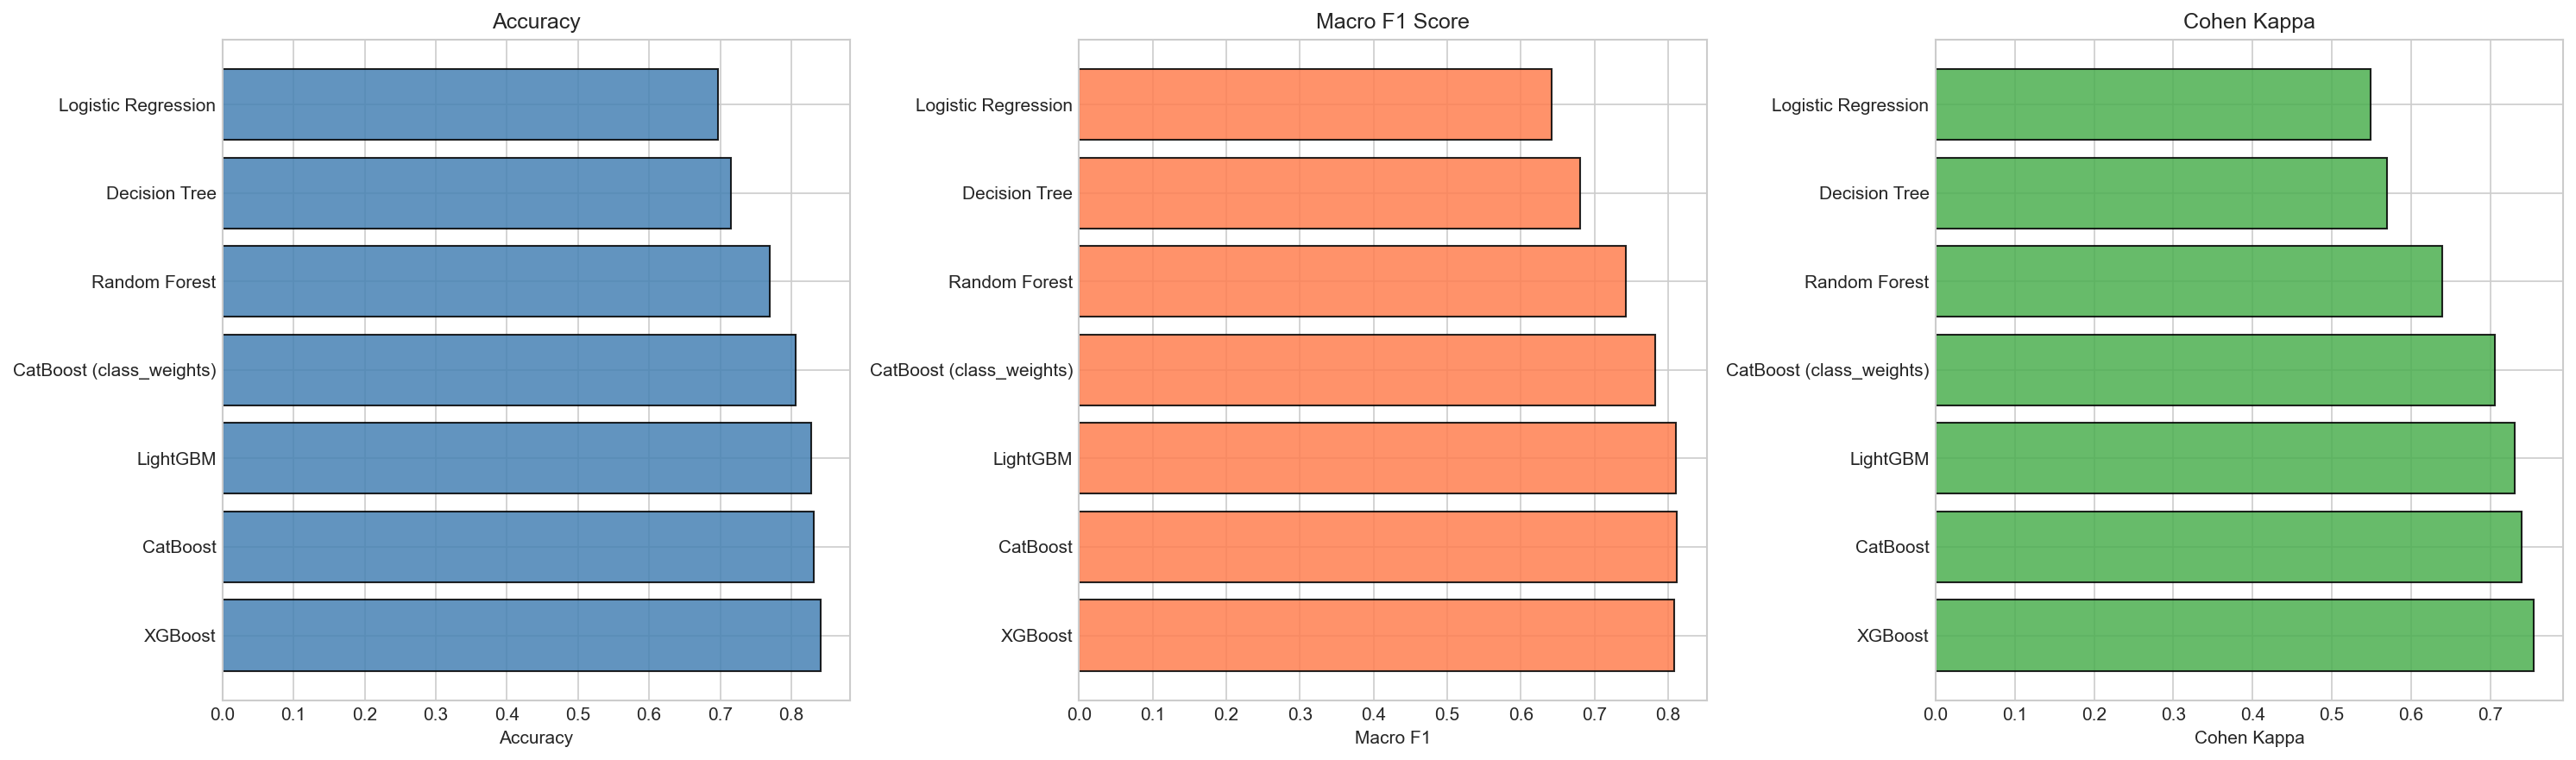
\includegraphics[width=\textwidth]{figures/19_classification_comparison.png}
\caption{Accuracy, Macro $F_1$, and Cohen's $\kappa$ comparison across all classification models.}
\label{fig:cls_comparison}
\end{figure}

\begin{figure}[H]
\centering
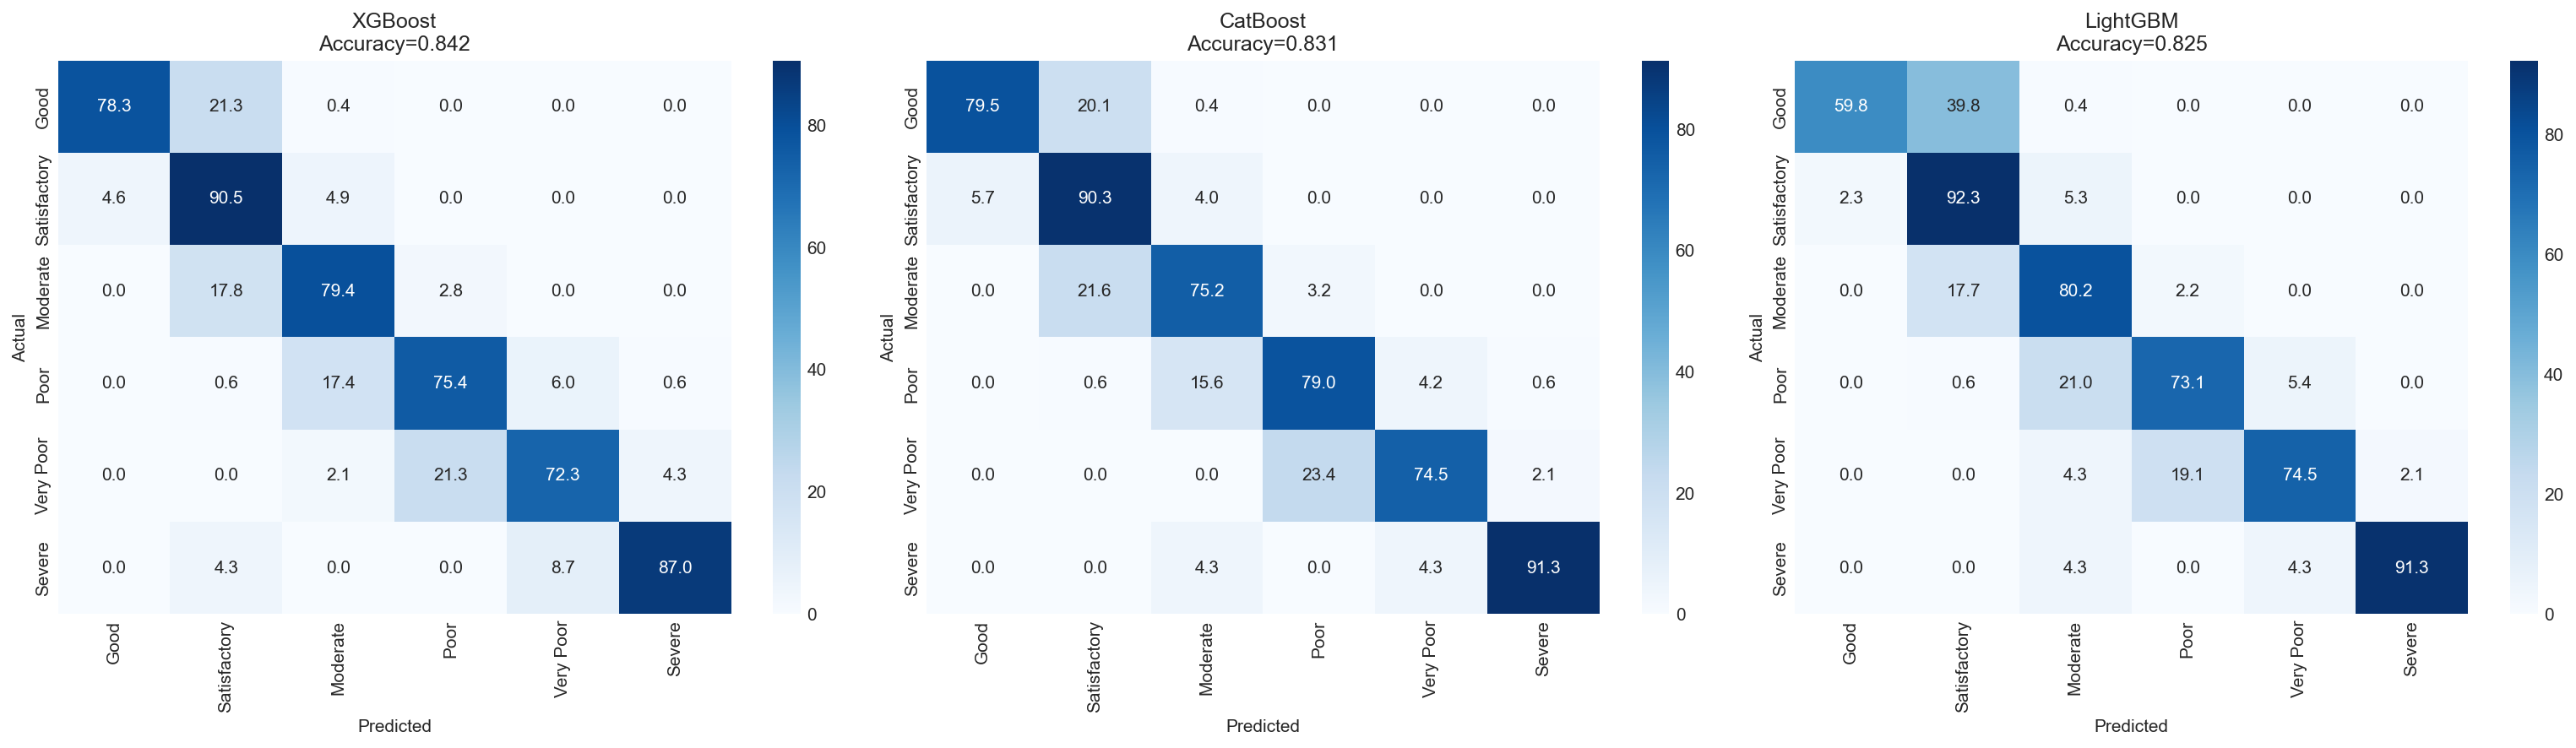
\includegraphics[width=\textwidth]{figures/20_confusion_matrices.png}
\caption{Normalised confusion matrices for the top three classifiers. Misclassifications are concentrated between adjacent AQI categories.}
\label{fig:confusion}
\end{figure}

Confusion matrix analysis (Figure~\ref{fig:confusion}) confirms that misclassifications are almost exclusively between adjacent categories (e.g., Satisfactory $\leftrightarrow$ Moderate, Poor $\leftrightarrow$ Very Poor). This is expected given the ordinal nature of the AQI scale: the boundary between Satisfactory (AQI 100) and Moderate (AQI 101) is a single-unit threshold in a noisy, continuous measurement.

\textbf{SMOTE vs.\ Class Weights.} The SMOTE-based CatBoost model outperformed its class-weighted counterpart: accuracy 0.831 vs.\ 0.804 (+2.7\%), $\kappa$ 0.739 vs.\ 0.704 (+0.035). This provides empirical evidence that synthetic oversampling is more effective than cost-sensitive learning for this multi-class ordinal target.

\section{Deep Learning Results}

Table~\ref{tab:dl_results} presents the deep learning model performance.

\begin{table}[H]
\centering
\caption{Deep Learning Model Performance on Test Set}
\label{tab:dl_results}
\begin{tabular}{|l|c|c|c|c|}
\hline
\textbf{Architecture} & \textbf{$R^2$} & \textbf{RMSE} & \textbf{MAE} & \textbf{Epochs} \\
\hline
Stacked LSTM & 0.6732 & 39.93 & 19.92 & 32 \\
\hline
Conv1D-LSTM & 0.6629 & 40.55 & 20.61 & 27 \\
\hline
Vanilla LSTM & 0.6560 & 40.97 & 19.29 & 54 \\
\hline
Bidirectional LSTM & 0.6373 & 42.07 & 19.66 & 28 \\
\hline
GRU & 0.6342 & 42.24 & 20.31 & 41 \\
\hline
\end{tabular}
\end{table}

The best deep learning model (Stacked LSTM, $R^2 = 0.6732$) underperforms LightGBM ($R^2 = 0.9014$) by 22.8 percentage points. All five architectures converge within 27--54 epochs, but the performance ceiling remains substantially below gradient boosting methods.

\begin{figure}[H]
\centering
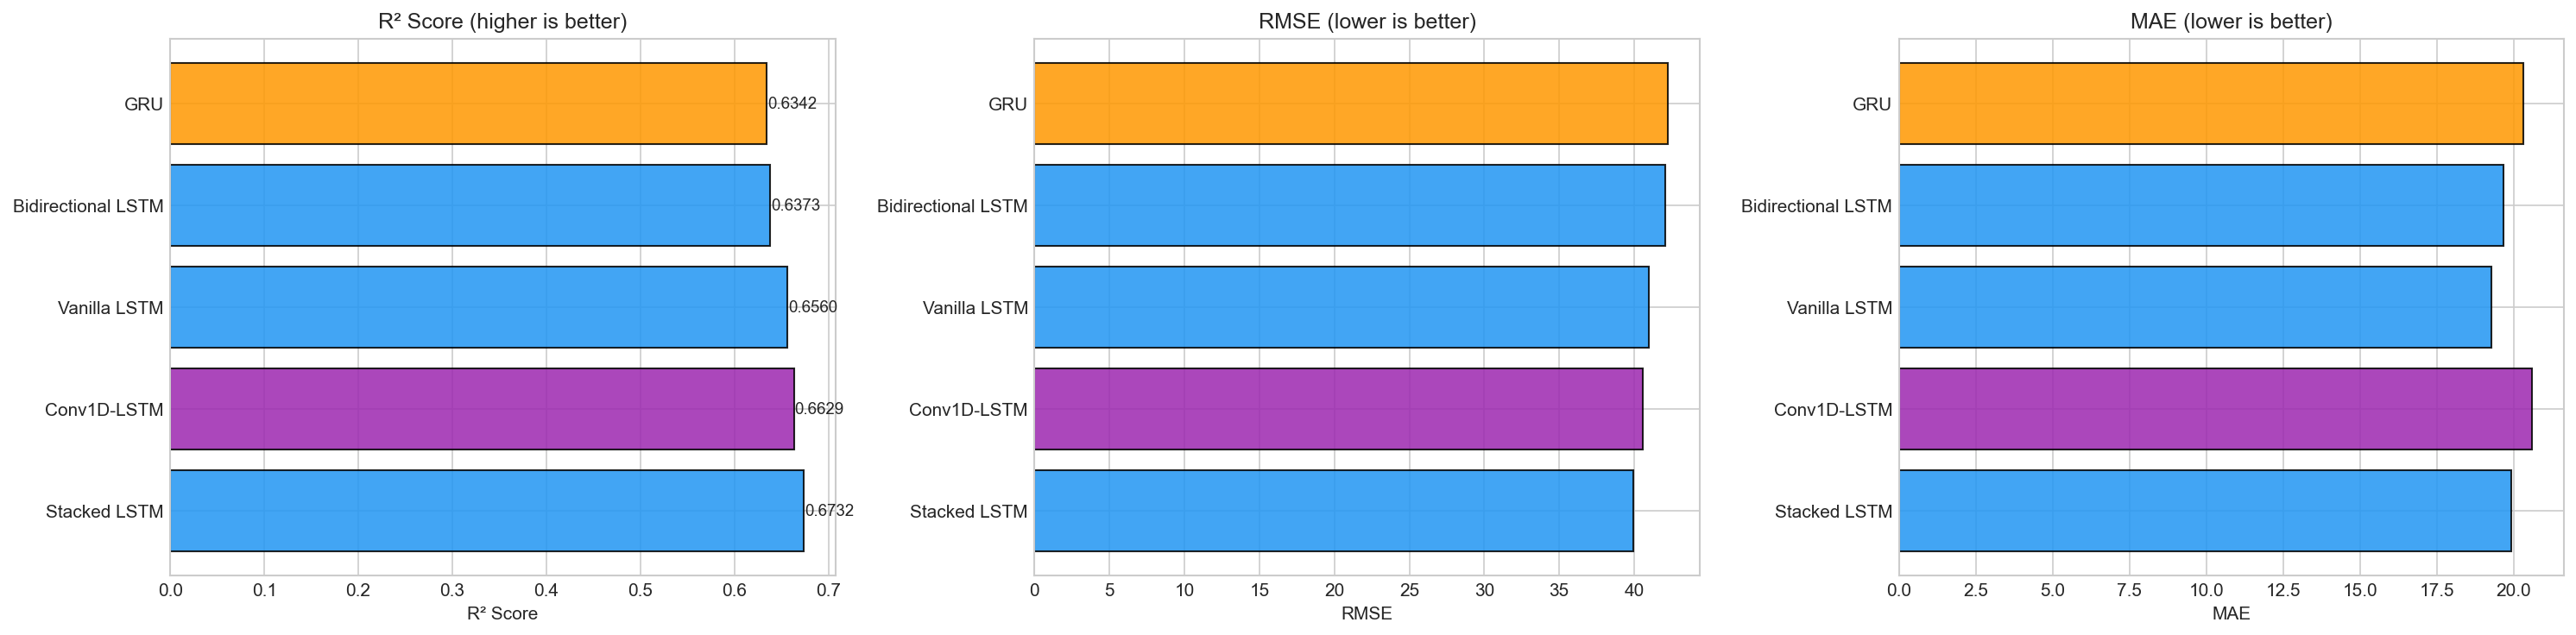
\includegraphics[width=\textwidth]{figures/21_dl_comparison.png}
\caption{Deep learning model comparison by $R^2$ and RMSE.}
\label{fig:dl_comparison}
\end{figure}

\begin{figure}[H]
\centering
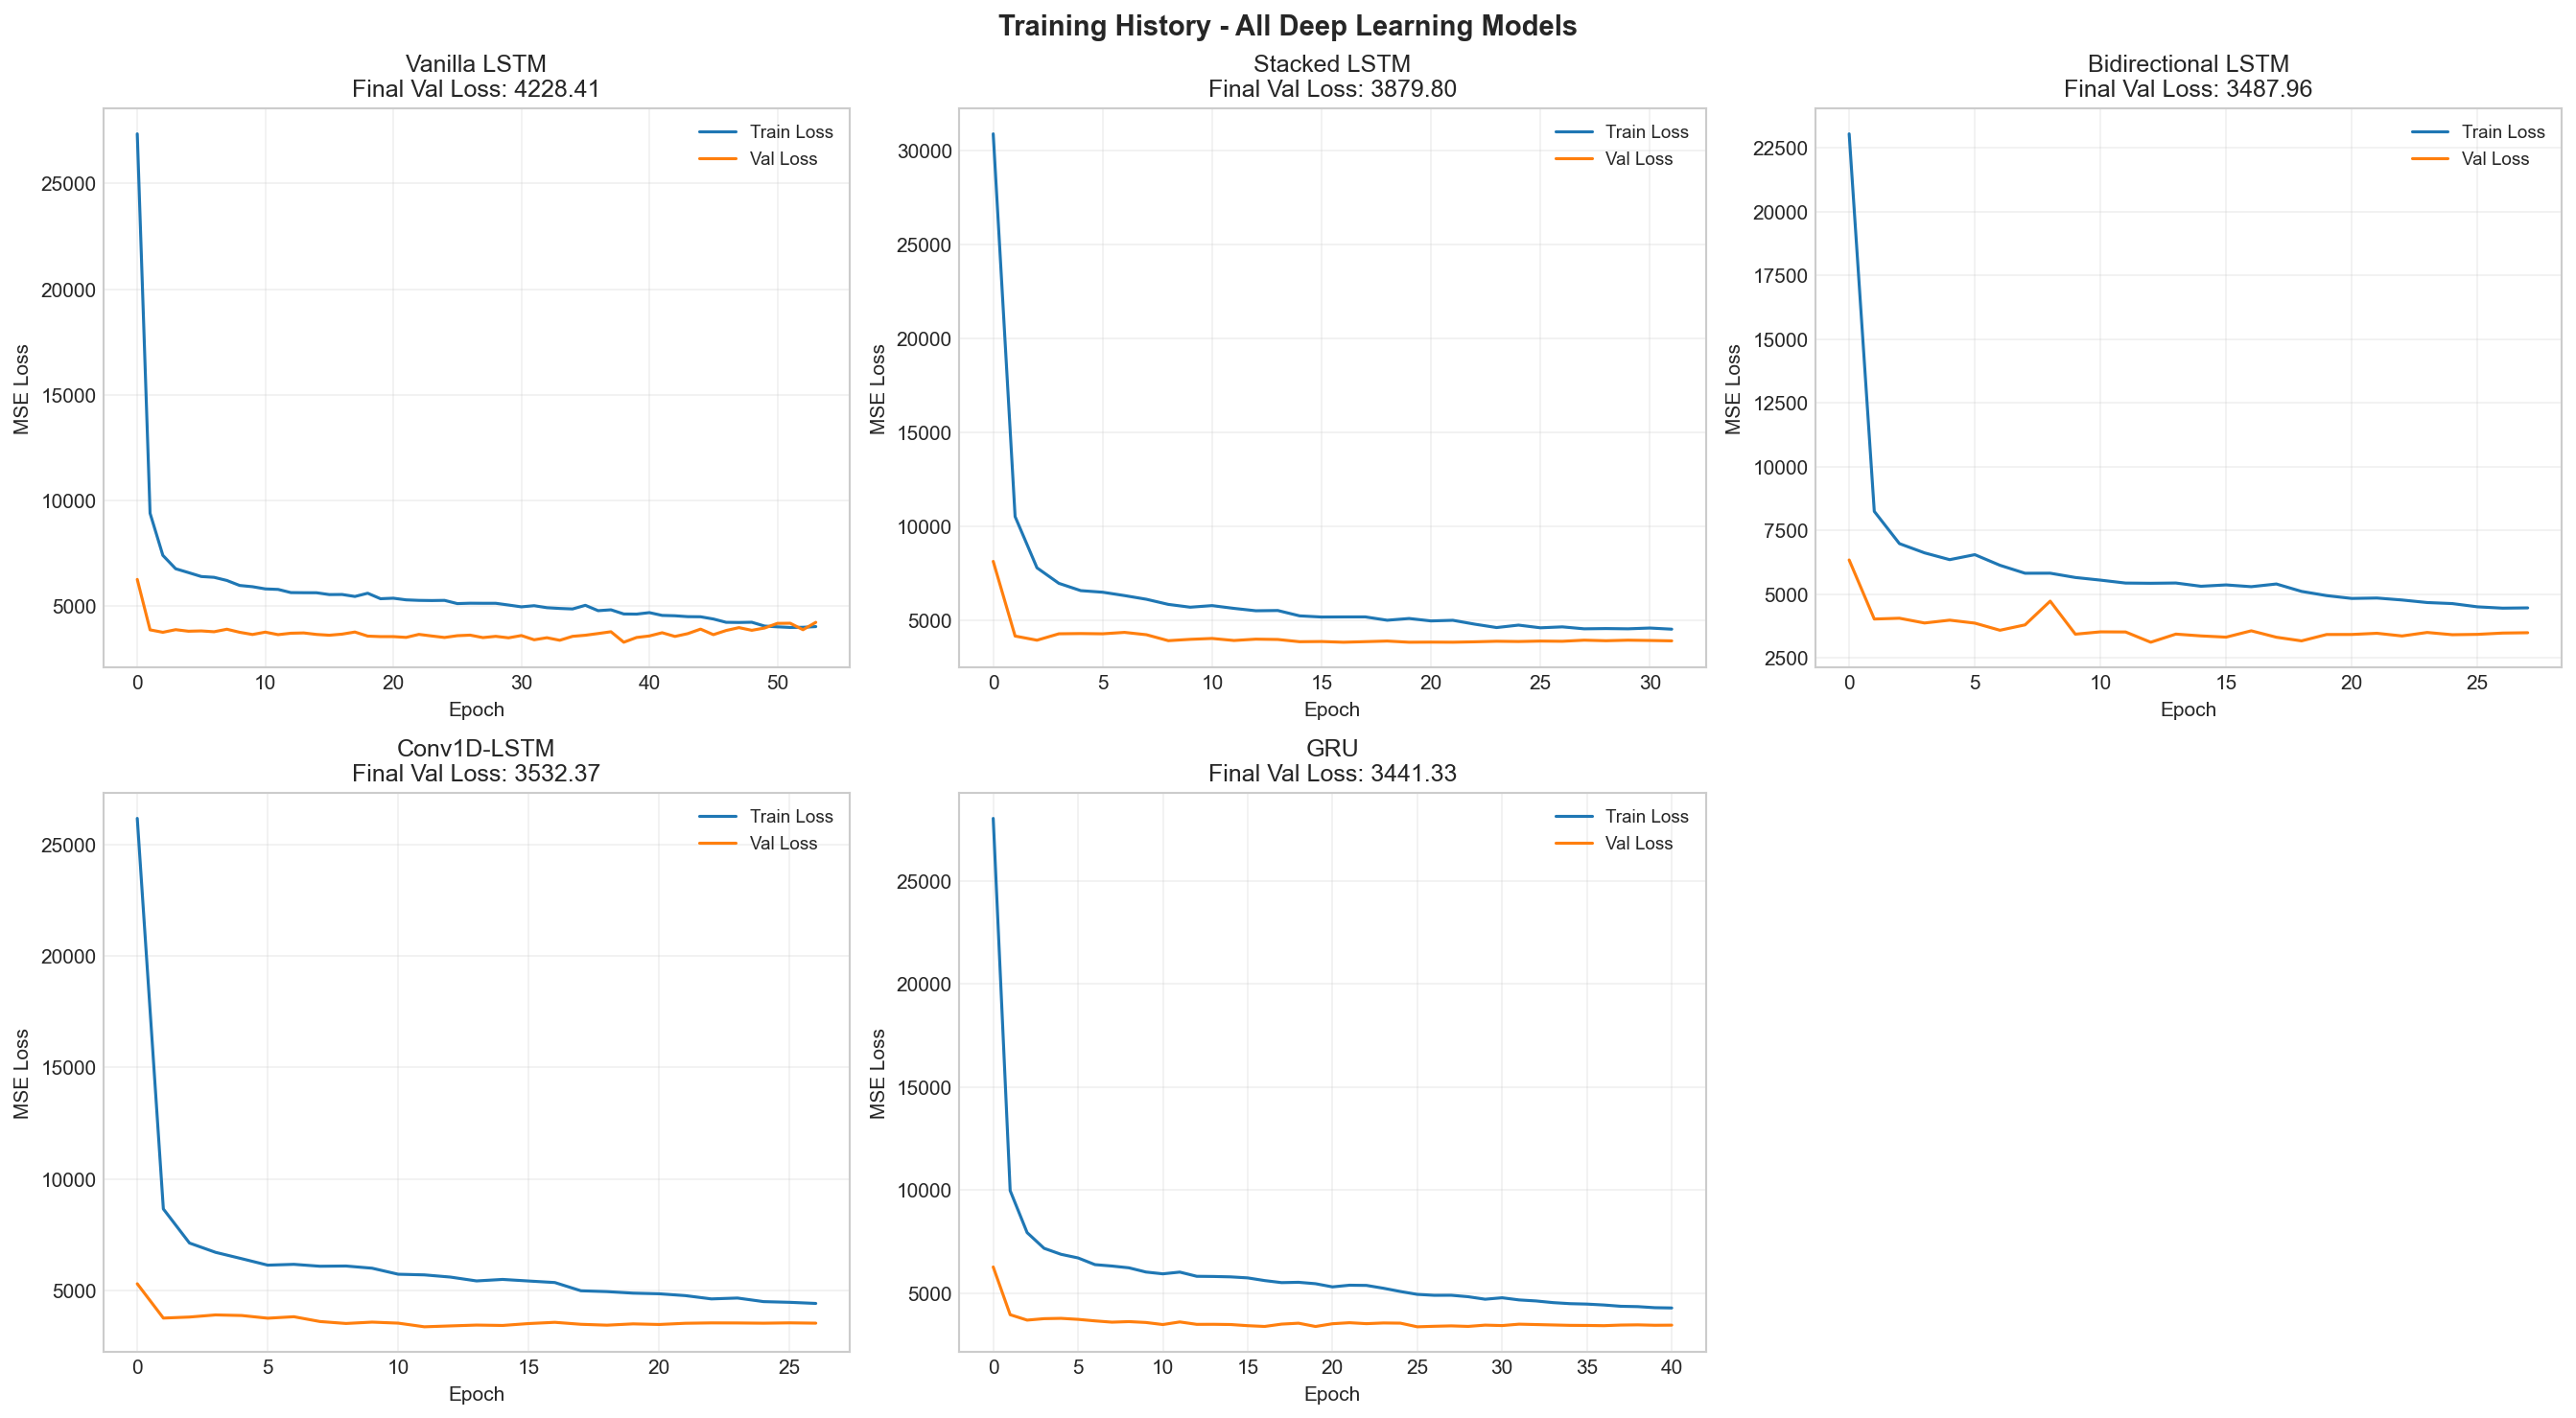
\includegraphics[width=\textwidth]{figures/22_dl_training_history.png}
\caption{Training and validation loss curves for all five deep learning architectures. All models converge within 30--55 epochs with early stopping.}
\label{fig:dl_history}
\end{figure}

The deep learning underperformance is attributable to two factors. First, the 72 lag features and 48 rolling statistics in the ML pipeline explicitly encode the temporal dependencies that LSTMs must learn implicitly from raw sequences of only 7 features over 14 timesteps --- a substantial information-theoretic disadvantage. Second, gradient boosting inherently performs feature selection through split-point optimisation, whereas LSTM dense layers assign non-zero weights to all input dimensions, including noisy or irrelevant pollutants. This finding corroborates Grinsztajn et al. (2022) and Shwartz-Ziv and Armon (2022): on tabular datasets with moderate dimensionality and sample sizes below 50,000, tree-based models decisively outperform neural networks.

\section{Hyperparameter Tuning}

Table~\ref{tab:optuna_results} presents the Optuna-tuned model performance.

\begin{table}[H]
\centering
\caption{Optuna-Tuned Regression Model Performance}
\label{tab:optuna_results}
\begin{tabular}{|l|c|c|c|c|}
\hline
\textbf{Model} & \textbf{$R^2$} & \textbf{RMSE} & \textbf{MAE} & \textbf{$\Delta R^2$} \\
\hline
\textbf{LightGBM (tuned)} & \textbf{0.9065} & \textbf{23.17} & \textbf{12.49} & +0.0051 \\
\hline
CatBoost (tuned) & 0.8576 & 28.60 & 15.35 & +0.0255 \\
\hline
XGBoost (tuned) & 0.7823 & 35.36 & 15.90 & +0.0331 \\
\hline
\end{tabular}
\end{table}

\begin{figure}[H]
\centering
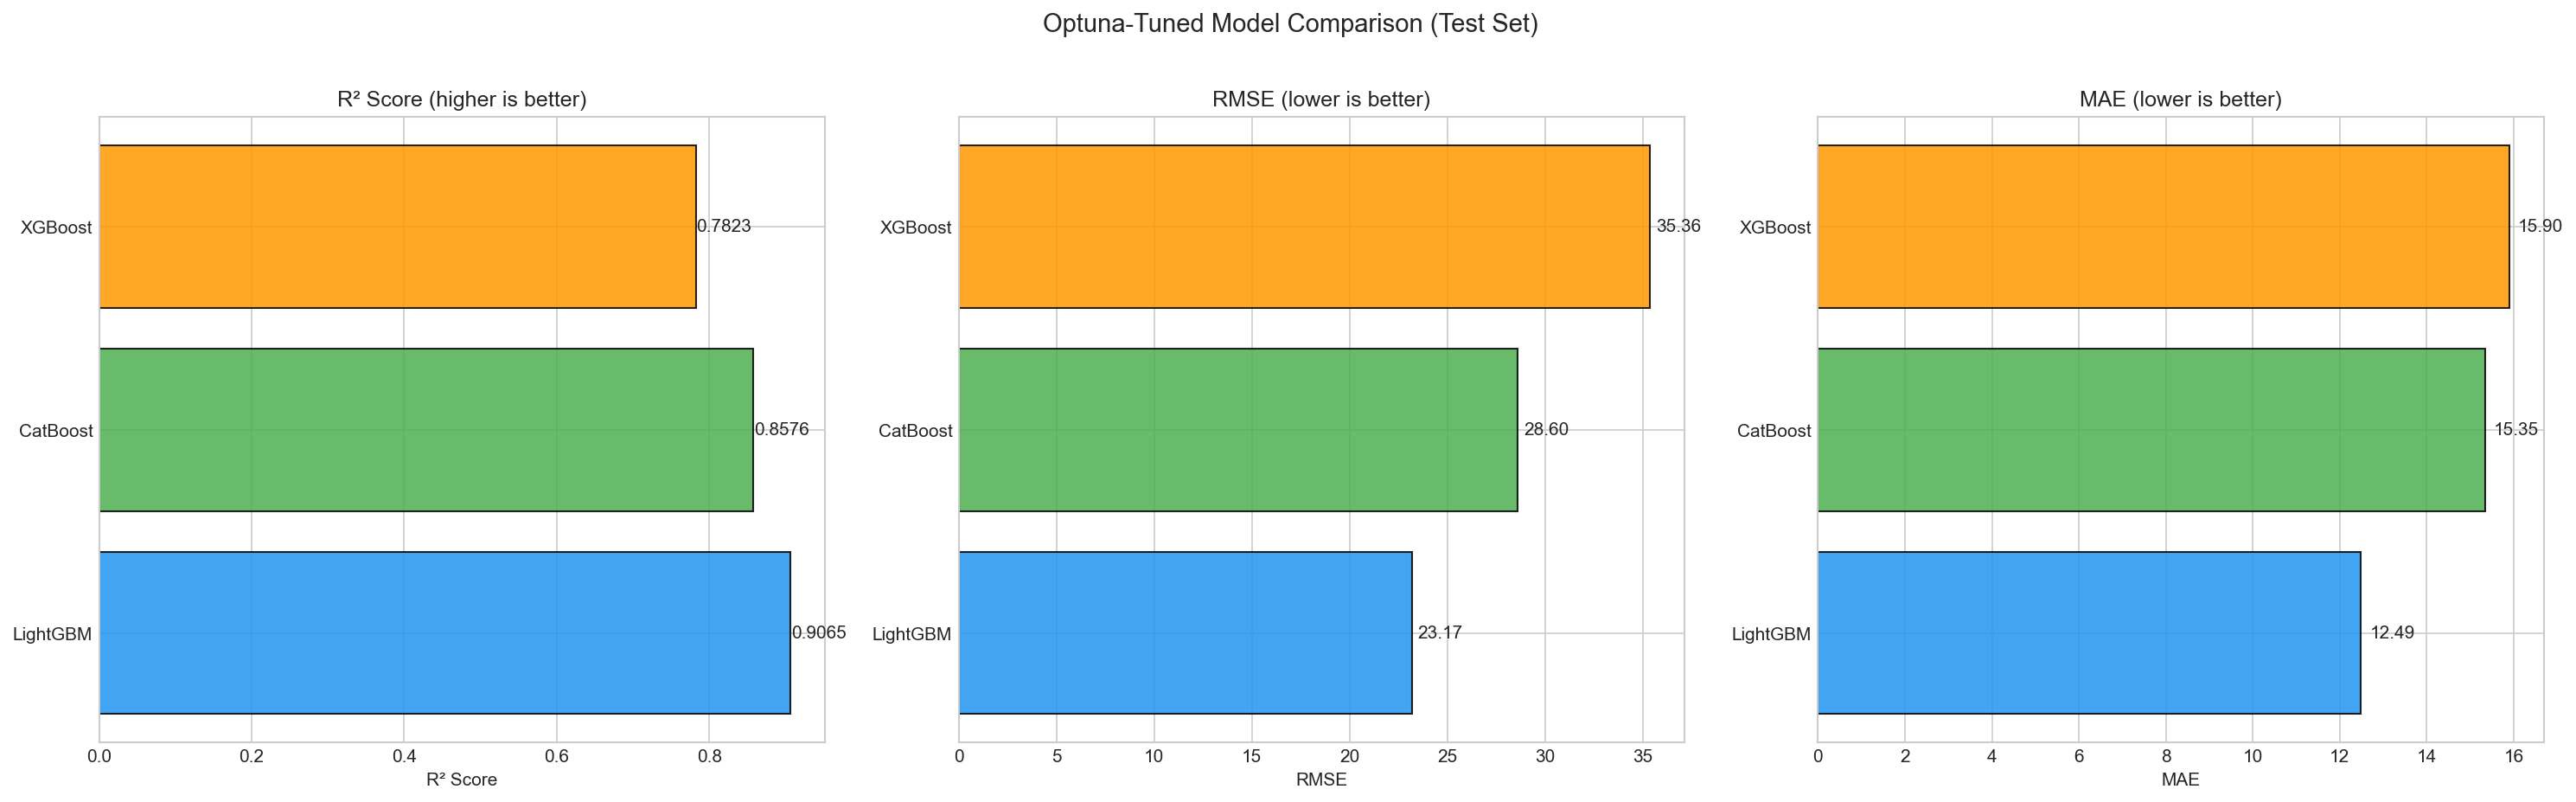
\includegraphics[width=\textwidth]{figures/25_optuna_comparison.png}
\caption{Baseline versus Optuna-tuned performance. LightGBM's improvement is marginal ($\Delta R^2 = 0.005$), while XGBoost benefits most ($\Delta R^2 = 0.033$).}
\label{fig:optuna}
\end{figure}

The tuned LightGBM achieved $R^2 = 0.9065$ (RMSE = 23.17), representing the best overall result. The marginal improvement for LightGBM ($\Delta R^2 = +0.005$) indicates that its default hyperparameters are already near-optimal for well-engineered features. CatBoost and XGBoost benefited more substantially from tuning ($\Delta R^2 = +0.026$ and $+0.033$, respectively), narrowing the gap to LightGBM but not closing it.

The primary conclusion is that the quality of feature engineering is the dominant determinant of predictive performance on this dataset, with hyperparameter tuning providing diminishing returns when default configurations are already well-calibrated.

\section{Cross-Paradigm Comparison}

\begin{figure}[H]
\centering
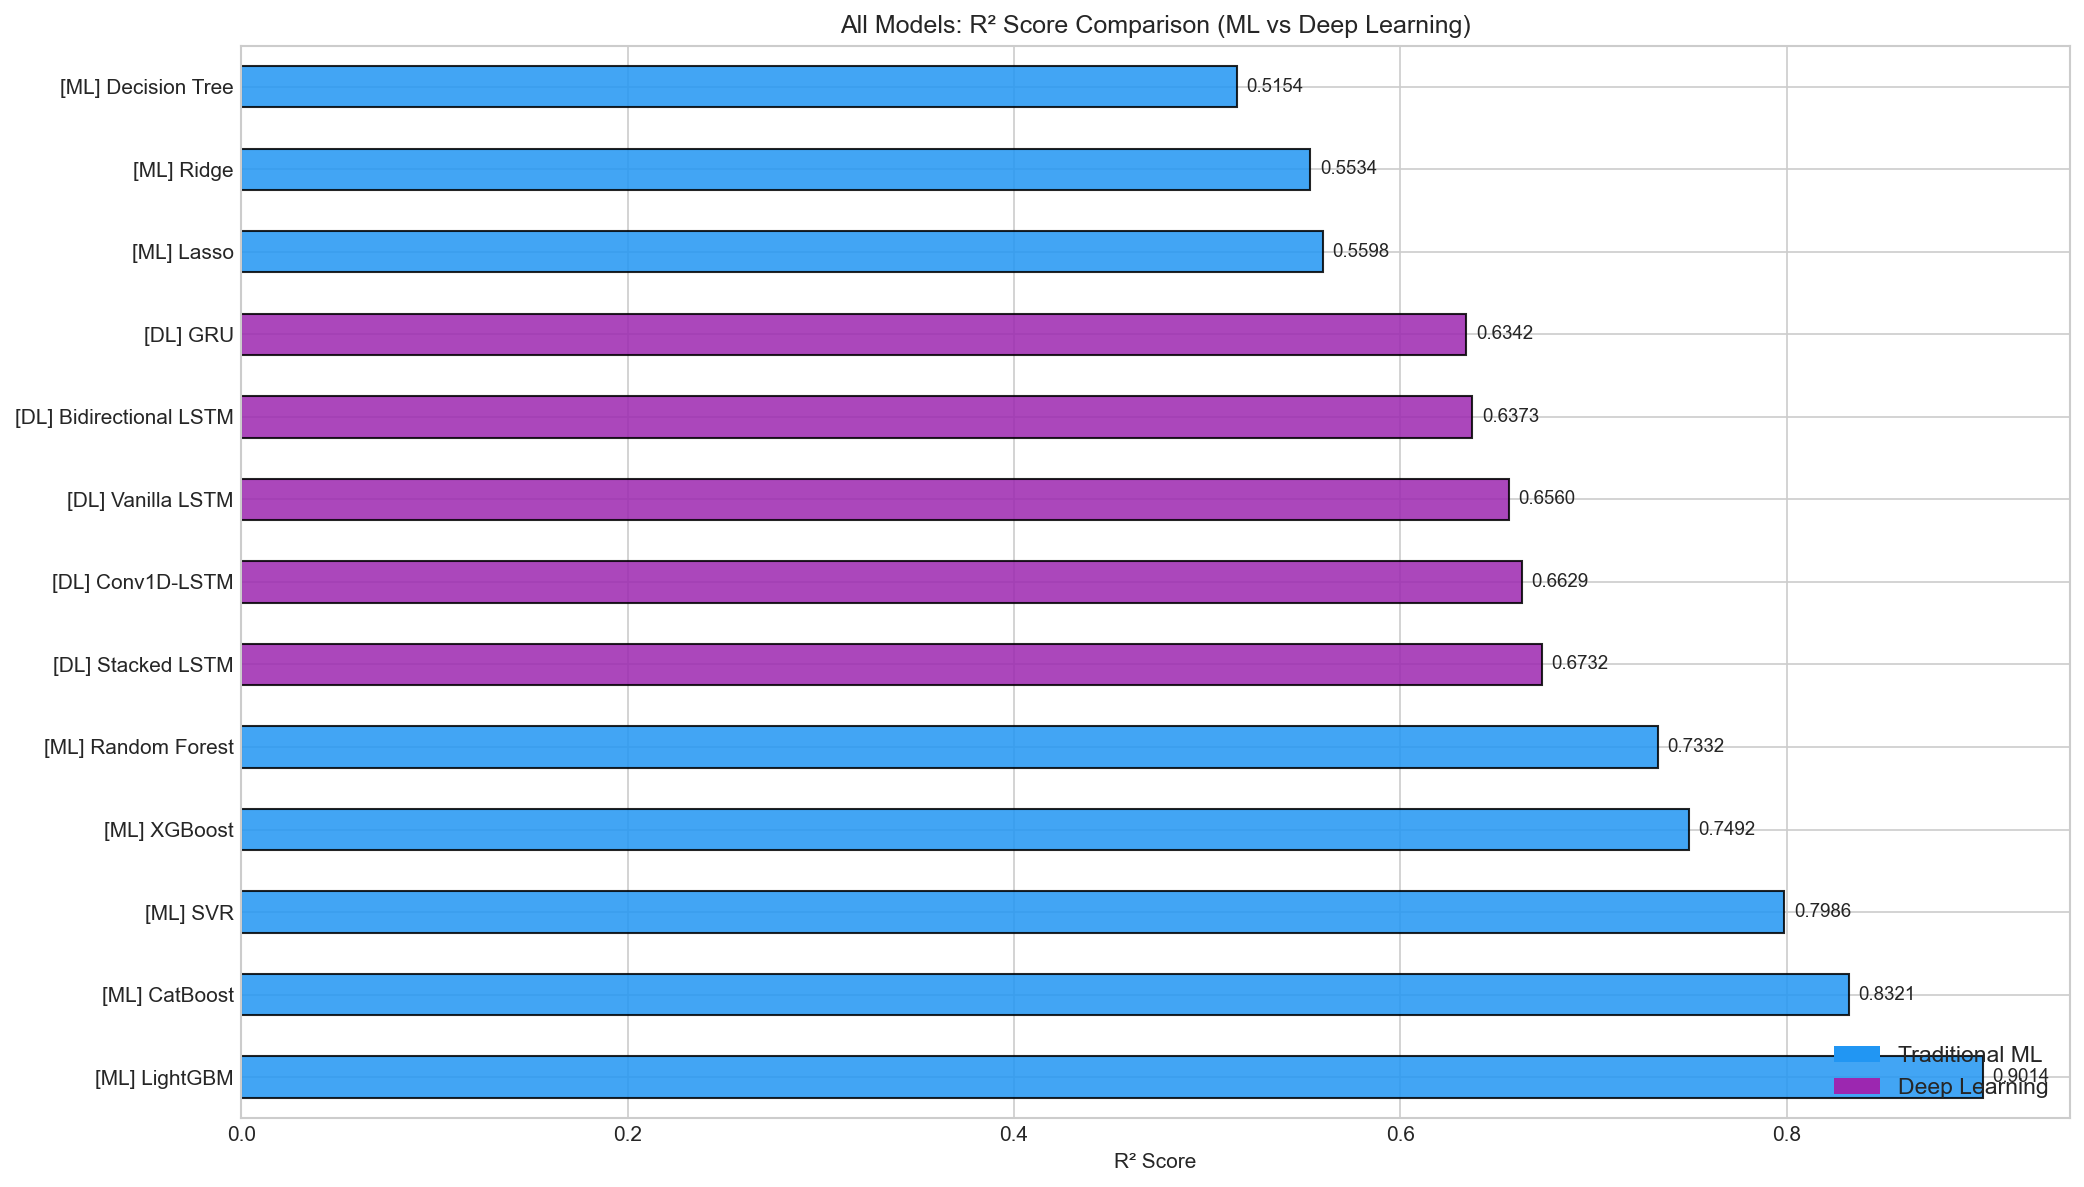
\includegraphics[width=\textwidth]{figures/24_all_models_comparison.png}
\caption{Unified comparison of all regression and deep learning models ranked by $R^2$, revealing a clear three-tier performance hierarchy.}
\label{fig:all_models}
\end{figure}

The unified comparison (Figure~\ref{fig:all_models}) reveals a clear three-tier hierarchy:

\begin{enumerate}
    \item \textbf{Tier 1 --- Gradient Boosting} ($R^2 = 0.75$--$0.90$): LightGBM, CatBoost, XGBoost, and SVR.
    \item \textbf{Tier 2 --- Deep Learning} ($R^2 = 0.63$--$0.67$): All five LSTM/GRU architectures.
    \item \textbf{Tier 3 --- Linear Methods} ($R^2 \approx 0.55$): Ridge, Lasso, and Decision Tree.
\end{enumerate}

The gap between Tier 1 and Tier 2 (approximately 23 percentage points) is the largest, indicating that the choice between gradient boosting and deep learning is the single most impactful modelling decision for this problem. The Tier 2 to Tier 3 gap (approximately 12 percentage points) quantifies the value of non-linear sequence modelling over purely linear approaches.

\section{Generated Graphs with Explanation}\label{idx:s61}

\begin{figure}[H]
\centering
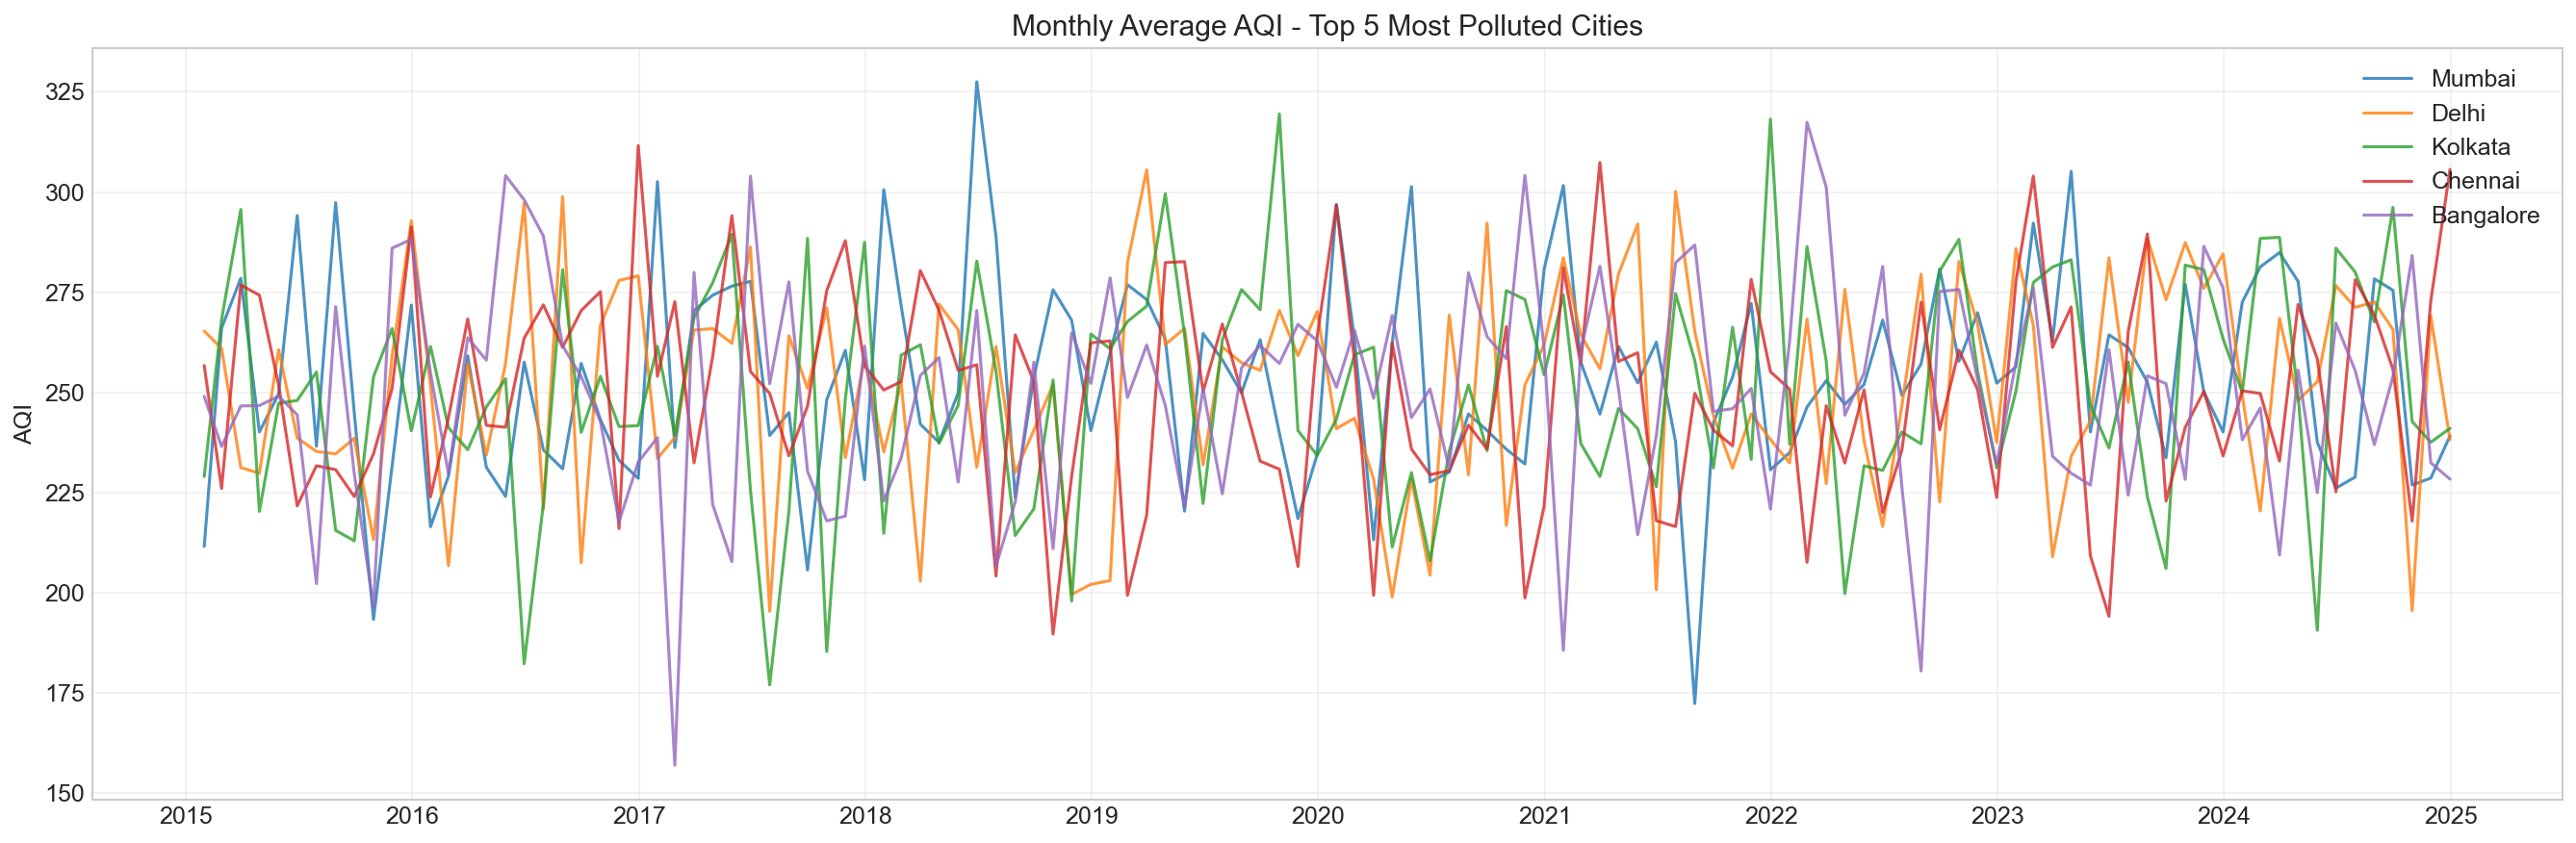
\includegraphics[width=\textwidth]{figures/07_top5_cities_timeseries.png}
\caption{Monthly average AQI for the five most polluted cities (Delhi, Patna, Lucknow, Jorapokhar, Kolkata). The sharp drop in early 2020 corresponds to India's COVID-19 lockdown.}
\label{fig:top5_cities}
\end{figure}

Figure~\ref{fig:top5_cities} presents the monthly average AQI time series for the five most polluted cities. Several patterns are evident: (1) strong annual seasonality with winter peaks and monsoon troughs, (2) Delhi consistently leading all cities in AQI, (3) the dramatic drop in March--May 2020 corresponding to the COVID-19 lockdown, which brought Delhi's AQI from its typical spring value of $\sim$180 down to $\sim$80, and (4) the October-November crop burning spike visible as a secondary peak each year.

\begin{figure}[H]
\centering
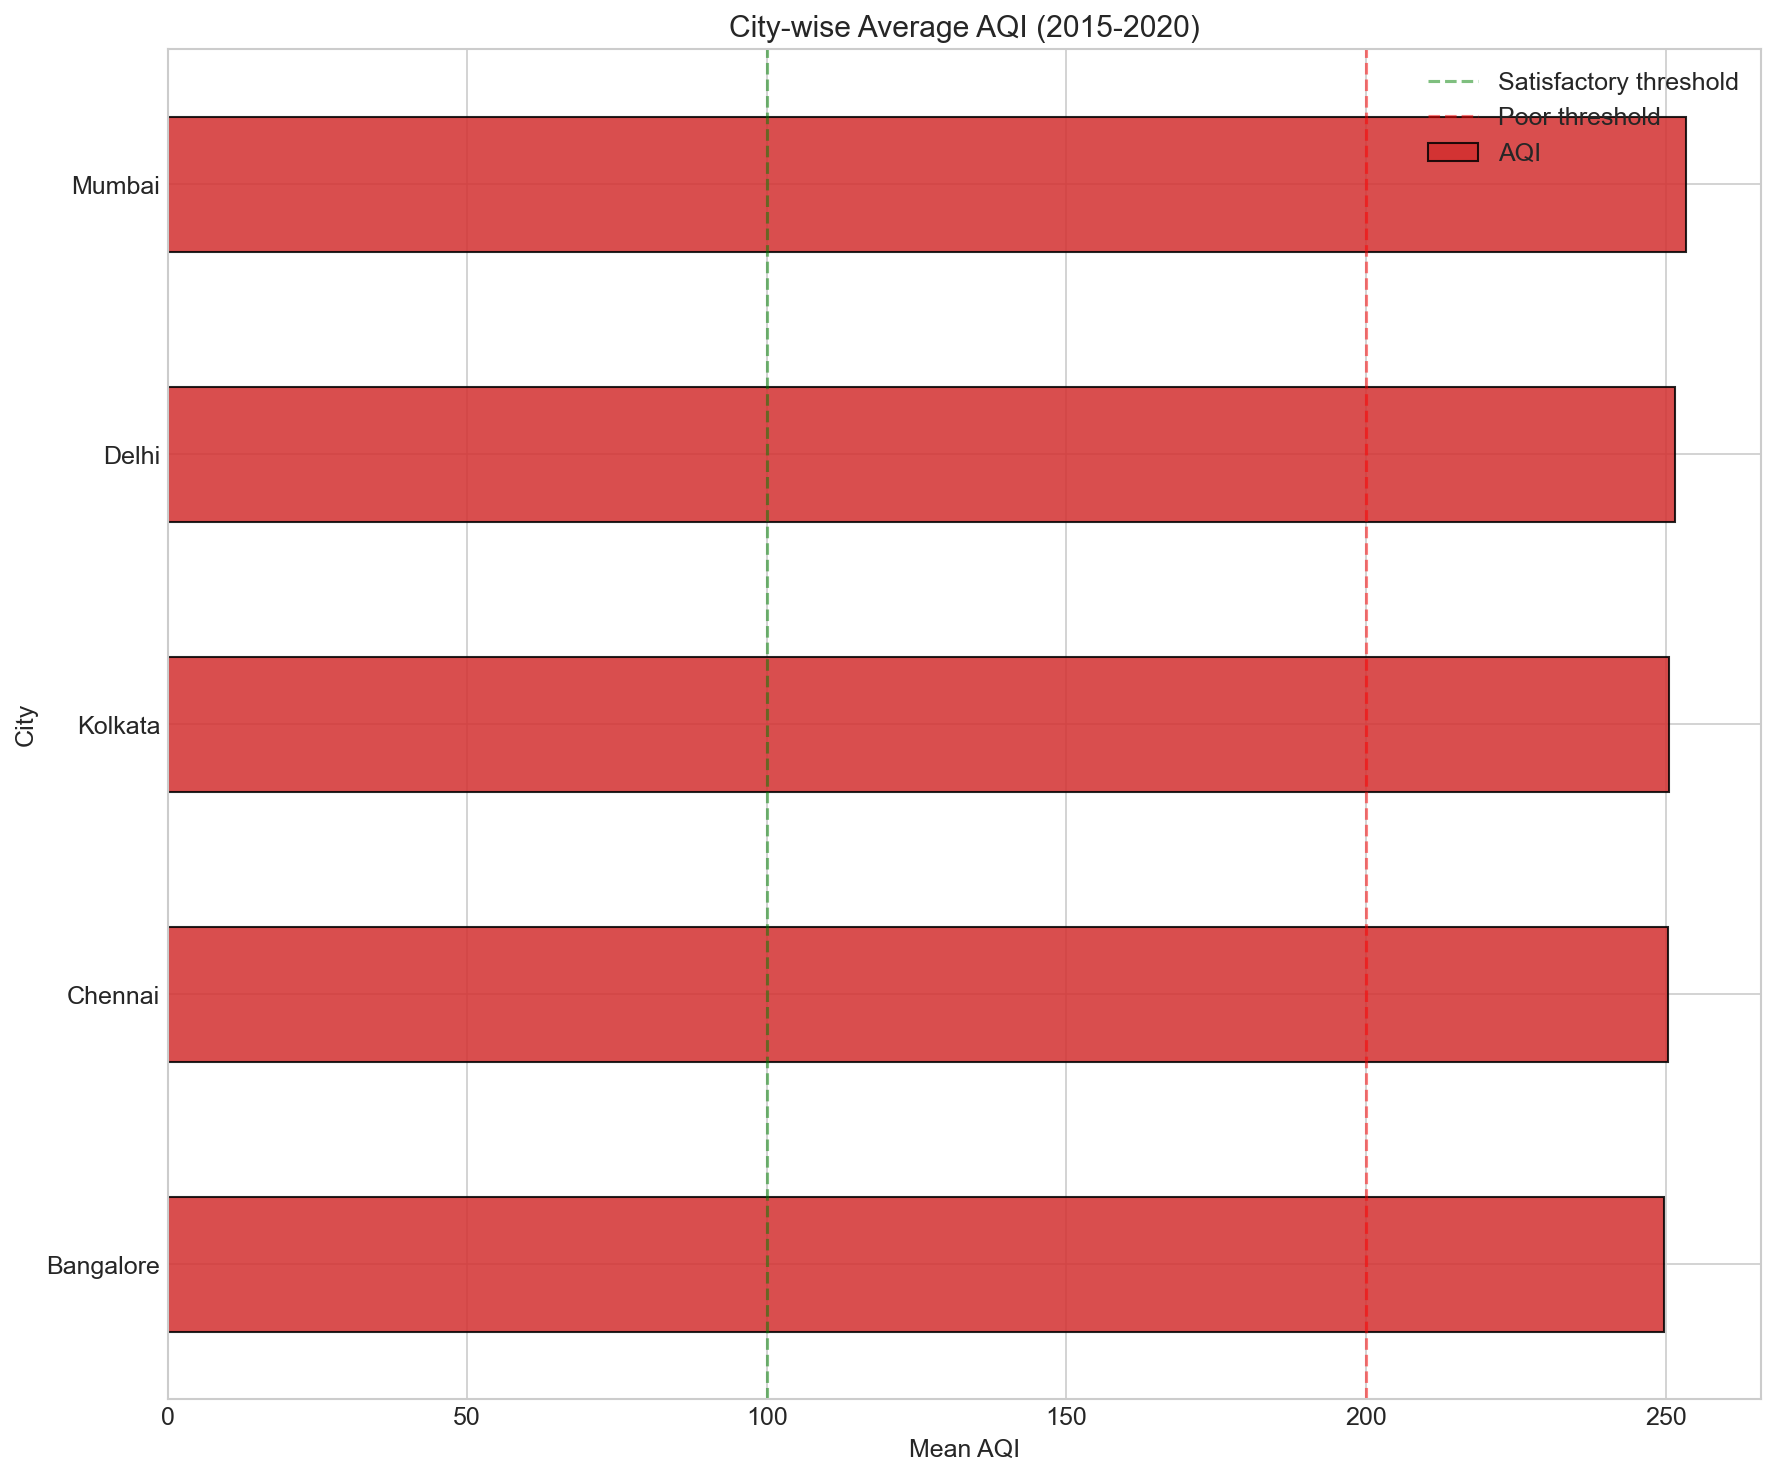
\includegraphics[width=\textwidth]{figures/08_city_mean_aqi.png}
\caption{City-wise average AQI (2015--2020). Delhi leads with a mean AQI exceeding 200, while northeastern and southern coastal cities maintain substantially lower levels.}
\label{fig:city_mean}
\end{figure}

Figure~\ref{fig:city_mean} presents the city-wise average AQI over the entire study period. The geographic gradient is striking: Indo-Gangetic Plain cities (Delhi, Patna, Lucknow) average AQI values in the ``Poor'' category ($>$200), while coastal cities (Thiruvananthapuram, Kochi) and northeastern elevated cities (Shillong, Aizawl) remain in the ``Satisfactory'' range ($<$100). This 4$\times$ variation in baseline AQI across Indian cities underscores the importance of the city encoding feature in the ML models.

% %%%%%%%%%%%%%%%%%%%%%%%%%%%%%%%%%%%%%%%%%%%%%%%%%%%%%%%%%%%%
% EXPLAINABILITY (SHAP ANALYSIS) — Unnumbered, not in INDEX
% Content preserved but not counted as a chapter in the 10-chapter INDEX
% %%%%%%%%%%%%%%%%%%%%%%%%%%%%%%%%%%%%%%%%%%%%%%%%%%%%%%%%%%%%
\clearpage
\chapter*{Explainability (SHAP Analysis)}
\markboth{Explainability (SHAP Analysis)}{}

\section*{Global Feature Importance}

\begin{figure}[H]
\centering
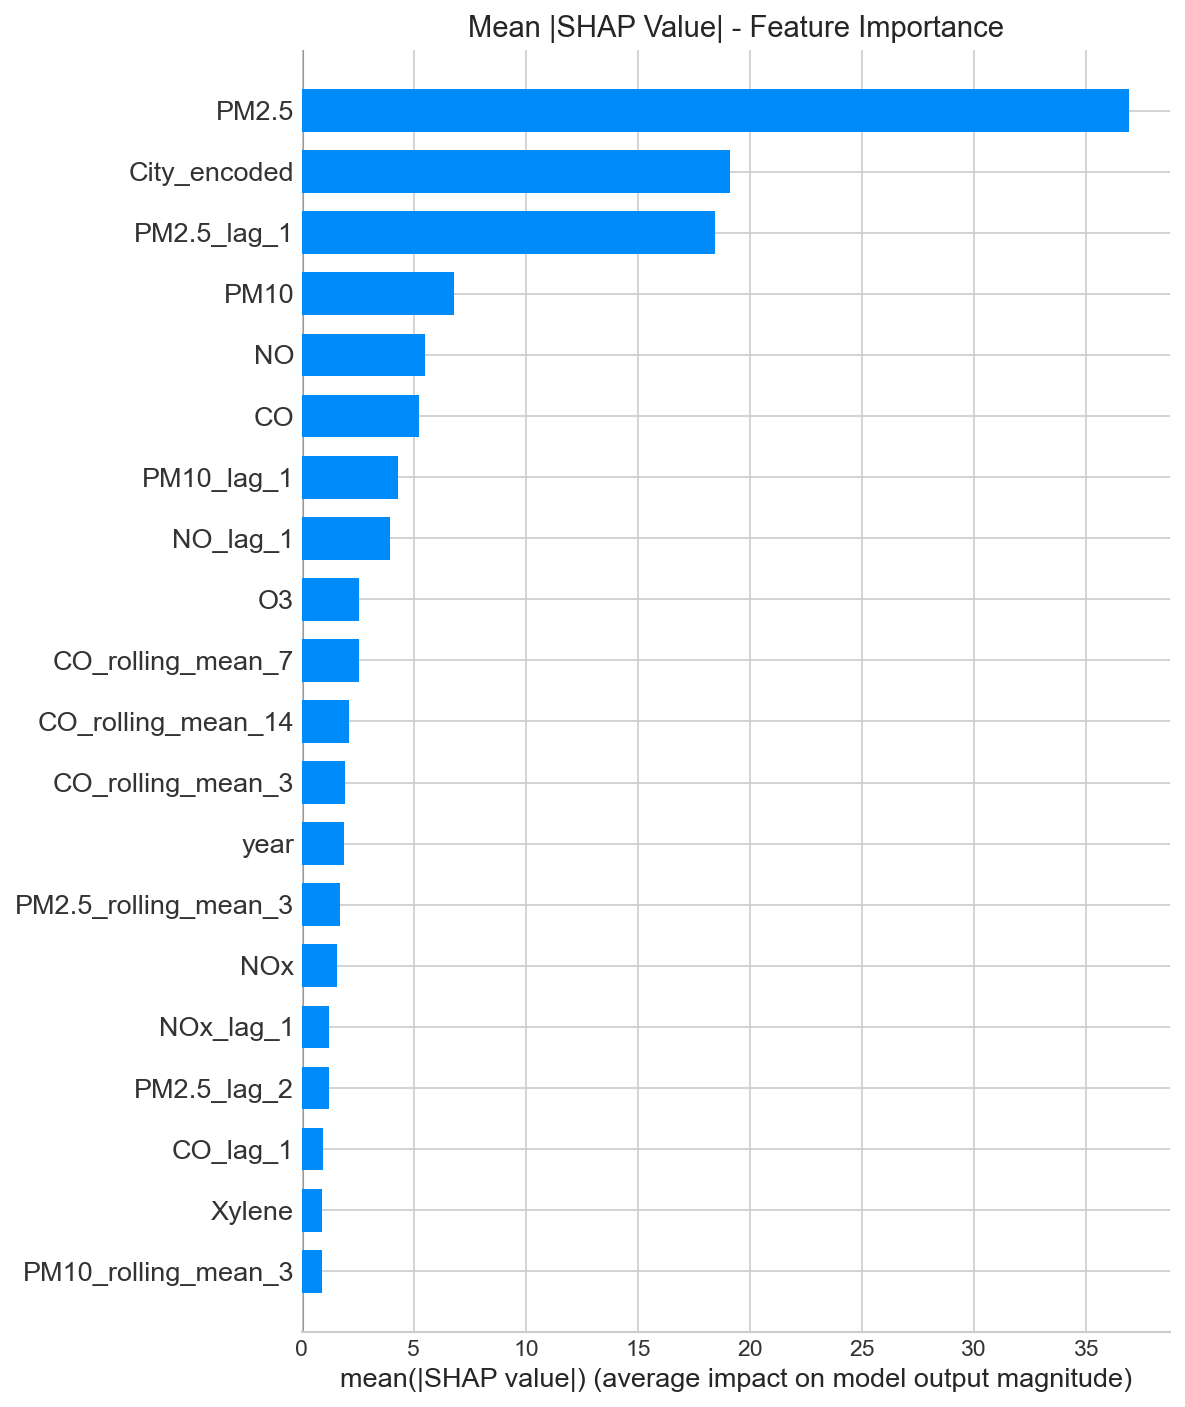
\includegraphics[width=\textwidth]{figures/27_shap_bar.png}
\caption{Global feature importance via mean absolute SHAP values for the Optuna-tuned LightGBM model (500 test samples). PM$_{2.5}$ lag and rolling features dominate.}
\label{fig:shap_bar}
\end{figure}

Figure~\ref{fig:shap_bar} ranks features by mean $|\text{SHAP}|$ across 500 test observations. The top 10 features by mean absolute SHAP value are:

\begin{enumerate}
    \item PM$_{2.5}$ 1-day lag
    \item PM$_{2.5}$ 7-day rolling mean
    \item PM$_{2.5}$ 3-day rolling mean
    \item CO 7-day rolling mean
    \item PM$_{10}$ 1-day lag
    \item PM$_{2.5}$ 14-day rolling mean
    \item CO 3-day rolling mean
    \item Month
    \item City encoding
    \item Day of year
\end{enumerate}

PM$_{2.5}$-derived features collectively account for the largest share of model output variation, consistent with PM$_{2.5}$'s role as the dominant sub-index pollutant in 60--70\% of CPCB AQI computations. CO rolling statistics appear prominently in positions 4 and 7, reflecting CO's role as a tracer of combustion emissions. Month and season features rank within the top 10, confirming the strong seasonal modulation of Indian air quality. The city encoding feature captures baseline inter-city differences (e.g., Delhi's mean AQI of 235 versus Shillong's 44).

\section*{Feature Interaction Analysis}

\begin{figure}[H]
\centering
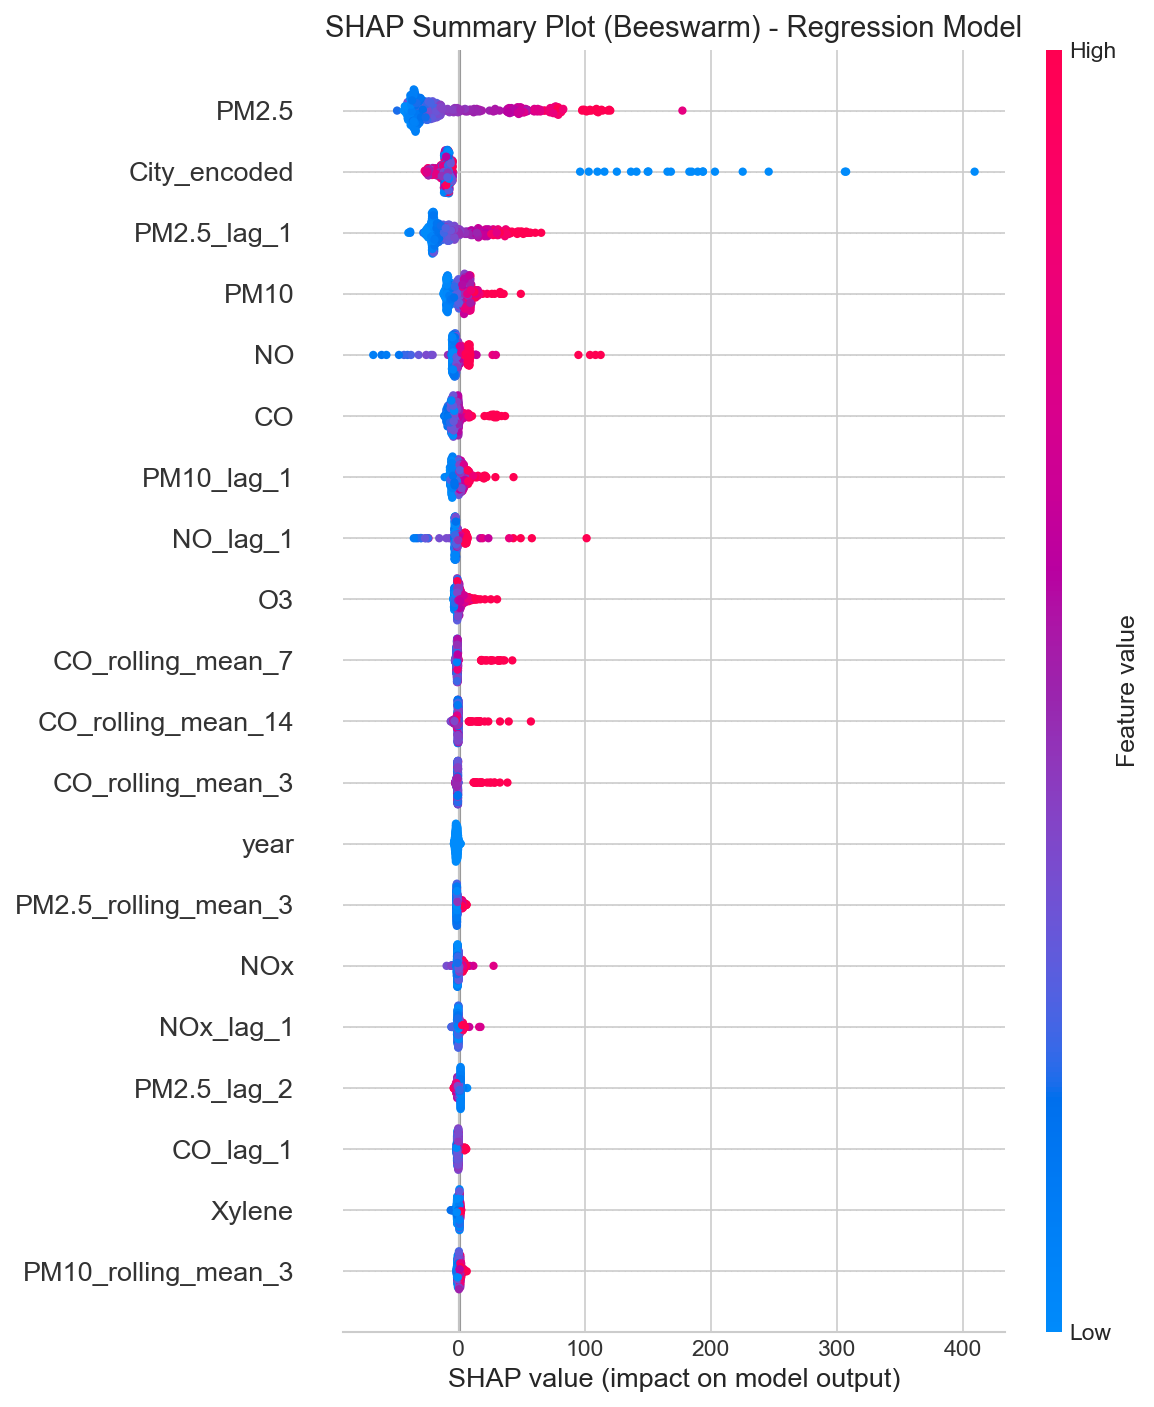
\includegraphics[width=\textwidth]{figures/26_shap_summary.png}
\caption{SHAP beeswarm plot showing per-instance feature contributions. Red = high feature value, blue = low. High PM$_{2.5}$ pushes SHAP values positive (higher predicted AQI); monsoon months push predictions negative.}
\label{fig:shap_beeswarm}
\end{figure}

The beeswarm plot (Figure~\ref{fig:shap_beeswarm}) reveals clear directional relationships between feature values and SHAP contributions:

\textbf{PM$_{2.5}$ lag features.} High raw values (red points) consistently produce positive SHAP contributions, pushing the predicted AQI upward. The relationship is monotonic and approximately linear at low-to-moderate concentrations but exhibits diminishing marginal impact at extreme values, consistent with the CPCB sub-index breakpoint structure where the AQI-per-$\mu$g/m$^3$ slope decreases at higher concentration brackets.

\textbf{Month feature.} A bimodal SHAP distribution is observed: winter months (November--February, appearing as high encoded values for months 11--12 and low for 1--2) produce positive SHAP contributions, while monsoon months (June--September) generate the strongest negative contributions. This pattern validates that the model has internalised India's seasonal pollution cycle.

\textbf{City feature.} Cities with high pollution baselines (encoded as specific integer values) produce positive SHAP contributions, while clean cities produce negative contributions. This captures the geographic heterogeneity that cannot be attributed to pollutant concentrations alone --- it reflects differences in emission density, topography, and meteorological ventilation.

\section*{Non-linear Effects}

\begin{figure}[H]
\centering
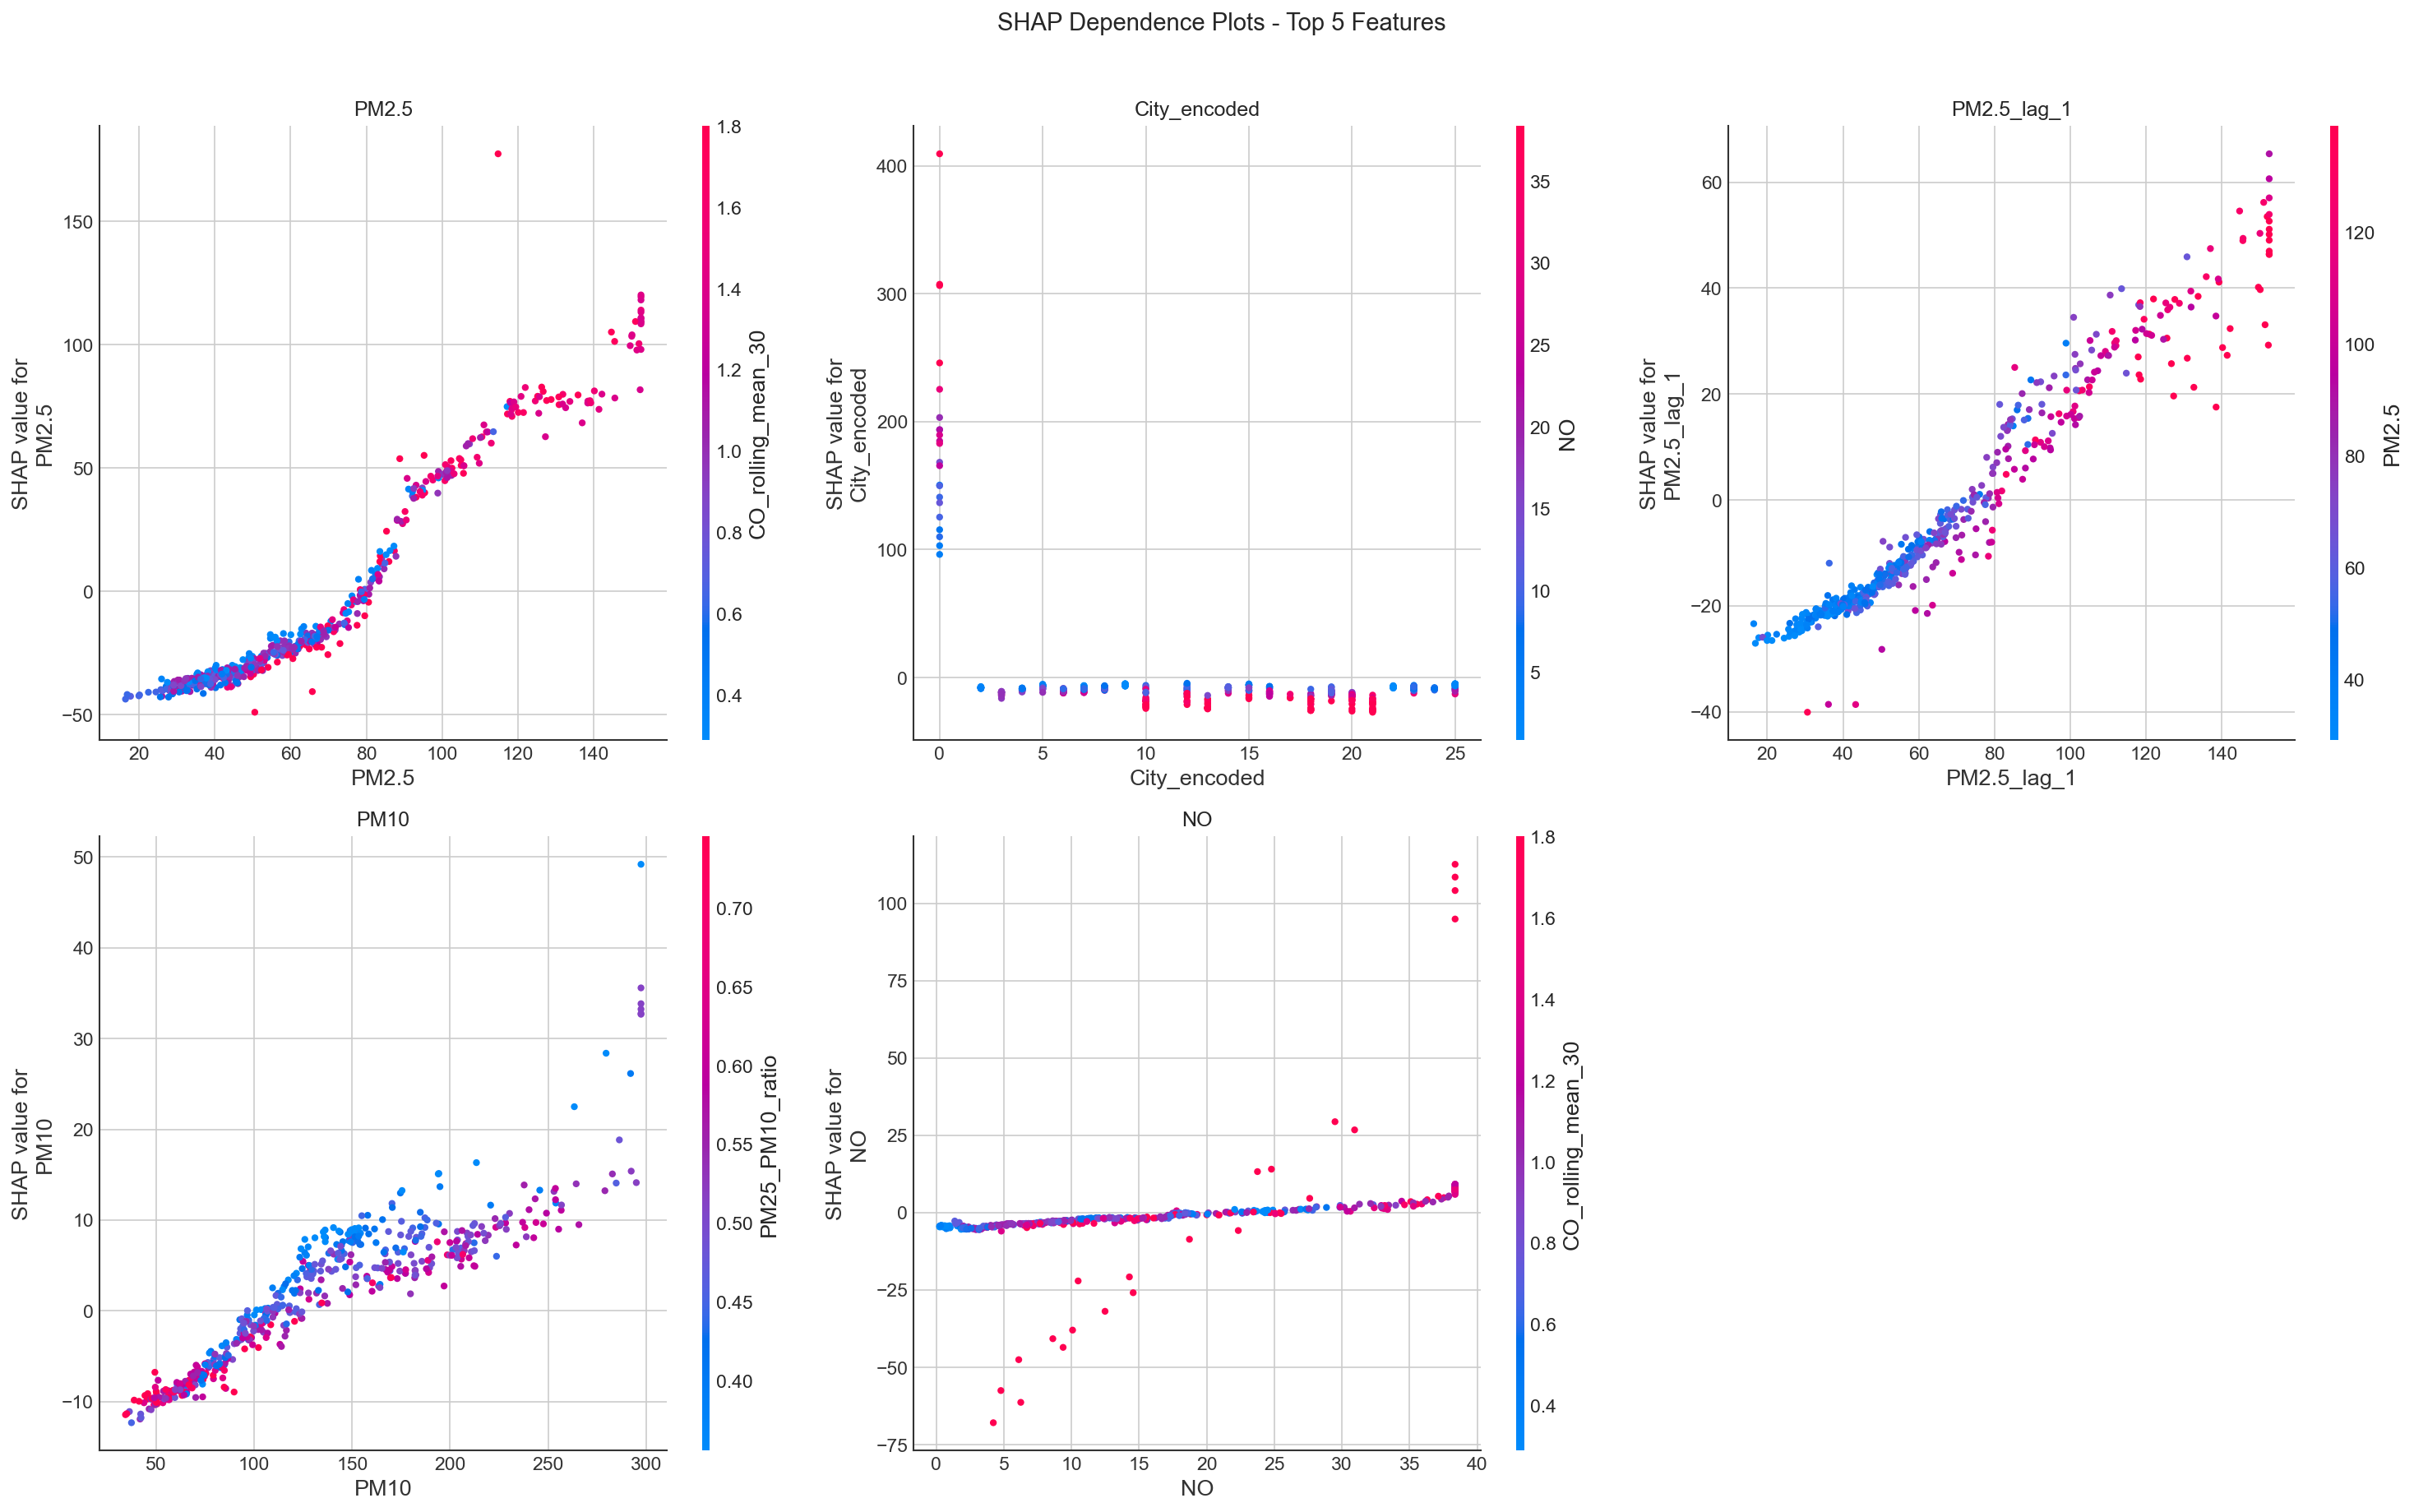
\includegraphics[width=\textwidth]{figures/28_shap_dependence.png}
\caption{SHAP dependence plots for top features with interaction colouring. PM$_{2.5}$ shows saturation above 250 $\mu$g/m$^3$; month shows V-shape with monsoon minimum.}
\label{fig:shap_dependence}
\end{figure}

Dependence plots (Figure~\ref{fig:shap_dependence}) expose non-linear feature-response relationships:

\textbf{PM$_{2.5}$ 1-day lag.} The SHAP value increases monotonically with lagged PM$_{2.5}$ concentration but exhibits a saturation effect above 250 $\mu$g/m$^3$. Interaction colouring reveals that co-elevation of PM$_{10}$ amplifies the positive SHAP contribution, indicating a synergistic effect when both fine and coarse particulate matter are simultaneously elevated --- characteristic of combined vehicular emissions and construction dust events.

\textbf{CO rolling mean.} CO SHAP values are near-zero below 1.0 mg/m$^3$ and increase steeply above 2.0 mg/m$^3$, consistent with a threshold-like behaviour: low-level CO indicates clean conditions, while elevated CO signals proximity to combustion sources.

\textbf{Month.} A V-shaped SHAP pattern is observed, with a minimum in July--August (monsoon washout) and maximum in November--December (post-monsoon crop burning and onset of winter inversions). The October--November increase is sharper than the March--April decrease, reflecting the abrupt onset of stubble burning versus the gradual improvement during spring.

\section*{Classification SHAP}

\begin{figure}[H]
\centering
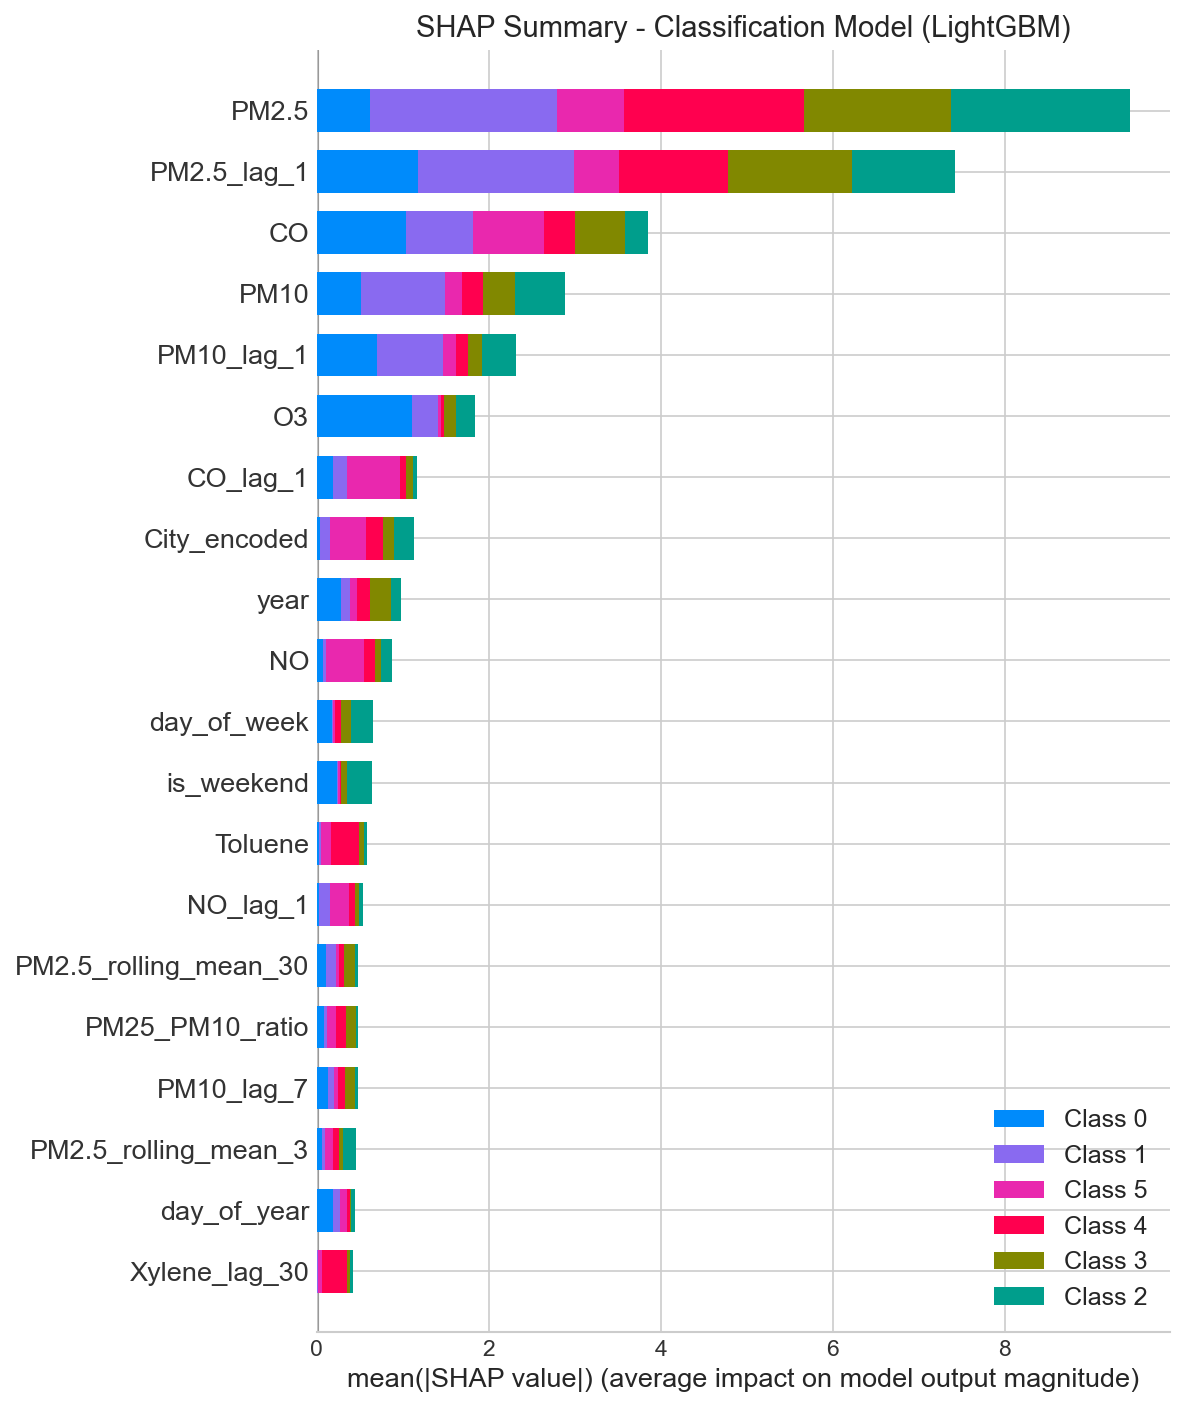
\includegraphics[width=\textwidth]{figures/29_shap_classification.png}
\caption{SHAP analysis for the XGBoost classifier, stratified by AQI category. Feature importance profiles differ markedly across categories.}
\label{fig:shap_class}
\end{figure}

Per-class SHAP analysis for the XGBoost classifier (Figure~\ref{fig:shap_class}) reveals category-specific feature profiles:

\textbf{Severe and Very Poor predictions} are driven almost entirely by PM$_{2.5}$ and CO lag features, which produce SHAP values 3--5$\times$ larger than for lower-severity categories. This indicates that extreme pollution events have distinctive, highly concentrated pollutant signatures.

\textbf{Good and Satisfactory predictions} rely more heavily on seasonal features and city encoding: monsoon season combined with a coastal or northeastern city shifts the prediction toward low-AQI categories even when some individual pollutant readings are moderately elevated.

This class-stratified analysis demonstrates that the model has learned distinct decision pathways for benign versus hazardous air quality conditions, rather than applying a single threshold-based rule.

\section*{Domain Validation}

The SHAP-derived feature importance hierarchy is validated against established atmospheric science through four confirmations:

\textbf{1. PM$_{2.5}$ Dominance.} PM$_{2.5}$ is the dominant sub-index pollutant in approximately 60--70\% of CPCB AQI computations, and its prominence in SHAP rankings confirms that the model has learned the actual AQI determination mechanism rather than spurious correlations.

\textbf{2. Seasonal Patterns.} The winter maximum / monsoon minimum in SHAP values mirrors the well-documented seasonal cycle of Indian air quality, driven by boundary layer dynamics (winter inversions vs.\ monsoon mixing), precipitation patterns (monsoon washout), and emission source variation (winter biomass burning, post-monsoon crop burning).

\textbf{3. CO as Combustion Tracer.} The prominence of CO features aligns with its established role as a marker for incomplete combustion from vehicular traffic, biomass cooking, and crop residue burning. The threshold effect identified by SHAP (CO $>$ 2.0 mg/m$^3$) is consistent with the CPCB breakpoint where CO transitions from ``Satisfactory'' to ``Moderate'' sub-index.

\textbf{4. Geographic Heterogeneity.} The high SHAP importance of the city encoding feature reflects genuine geographic variation: landlocked basin cities (Delhi, Patna) have fundamentally different pollutant dispersion characteristics compared to coastal (Mumbai, Kochi) or elevated (Shillong) locations. This is not a modelling artifact but a physical reality arising from topography, ventilation, and emission density.

% %%%%%%%%%%%%%%%%%%%%%%%%%%%%%%%%%%%%%%%%%%%%%%%%%%%%%%%%%%%%
% CHAPTER 7: MODEL OUTPUT (was 8 before Explainability became unnumbered)
% %%%%%%%%%%%%%%%%%%%%%%%%%%%%%%%%%%%%%%%%%%%%%%%%%%%%%%%%%%%%
\clearpage
\chapter{Model Output}\label{idx:ch7}

\section{Streamlit Dashboard Overview}\label{idx:s71}

The project culminates in a seven-page interactive Streamlit web application that serves as the primary interface for data exploration, model comparison, and live prediction. The dashboard is launched via \texttt{streamlit run app/app.py} and is accessible through any web browser.

\begin{table}[H]
\centering
\caption{Streamlit Dashboard Pages}
\label{tab:dashboard_pages}
\begin{tabular}{|c|l|p{7cm}|}
\hline
\textbf{Page} & \textbf{Name} & \textbf{Description} \\
\hline
1 & Home & Landing page with key metrics, project summary, and navigation \\
\hline
2 & Project Overview & Dataset information, pipeline description, technology stack \\
\hline
3 & EDA Visualisations & All 30 analytical figures organised by analysis section \\
\hline
4 & Model Comparison & Tabbed view: Regression / Classification / DL / Tuned / Overall \\
\hline
5 & Live Prediction & Manual pollutant input + WAQI API live city data + AQI gauge \\
\hline
6 & City Analysis & Historical trends, multi-city comparison, date range explorer \\
\hline
7 & Forecast \& Insights & 7-day AQI forecasts, causal analysis, Gemini AI insights \\
\hline
\end{tabular}
\end{table}

The dashboard integrates four external APIs: the World Air Quality Index (WAQI) API for real-time pollutant data, the Open-Meteo API for weather forecasts, the Google Gemini API for AI-powered insights, and Plotly for interactive visualisations. The application supports both manual input mode (pollutant sliders with preset configurations) and live mode (fetching real-time data for any of 26 Indian cities).

\begin{figure}[H]
\centering
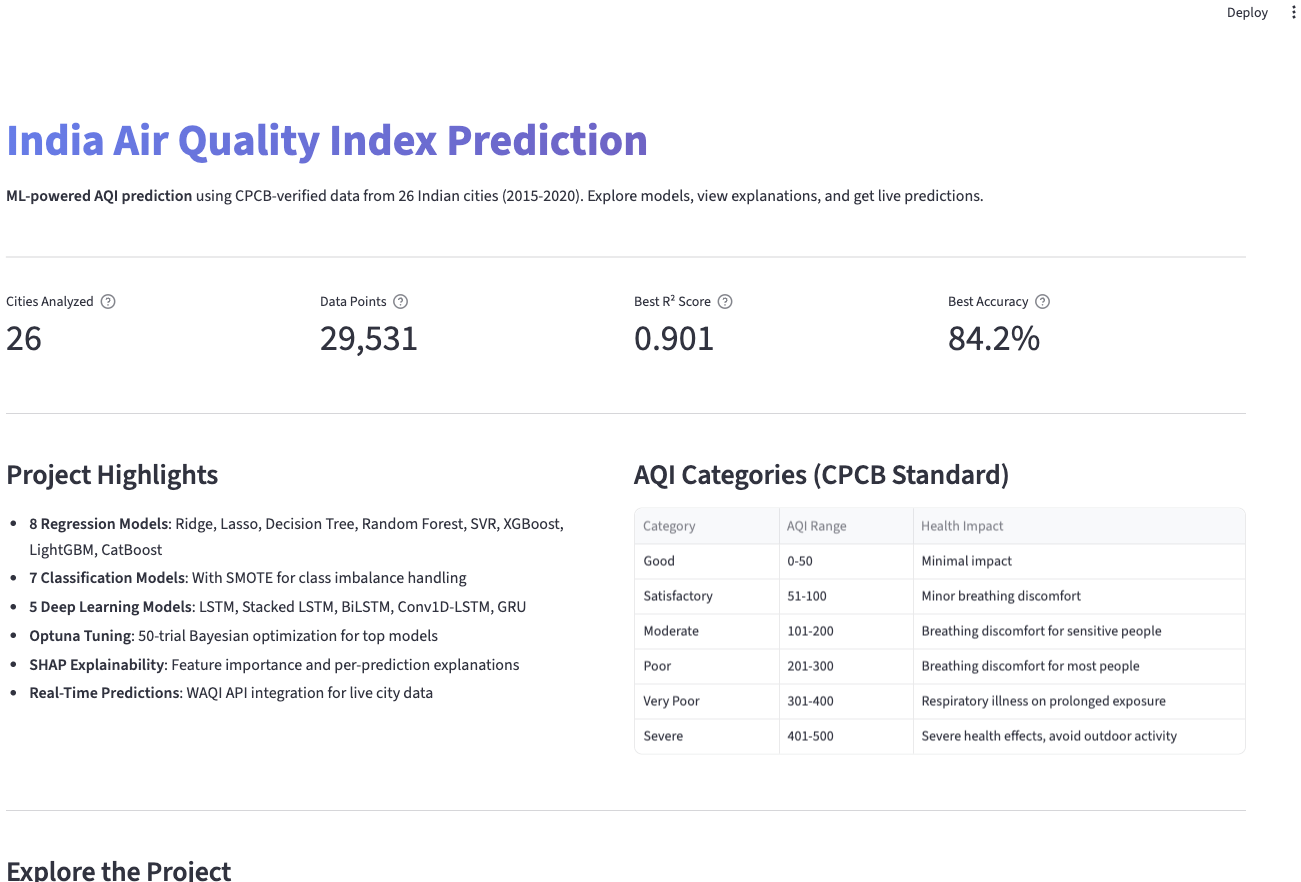
\includegraphics[width=\textwidth]{figures/ss_home.png}
\caption{Home page of the Streamlit dashboard showing key project metrics (26 cities, 29,531 data points, $R^2 = 0.901$, Accuracy = 84.2\%), project highlights, and AQI category reference table.}
\label{fig:ss_home}
\end{figure}

\begin{figure}[H]
\centering
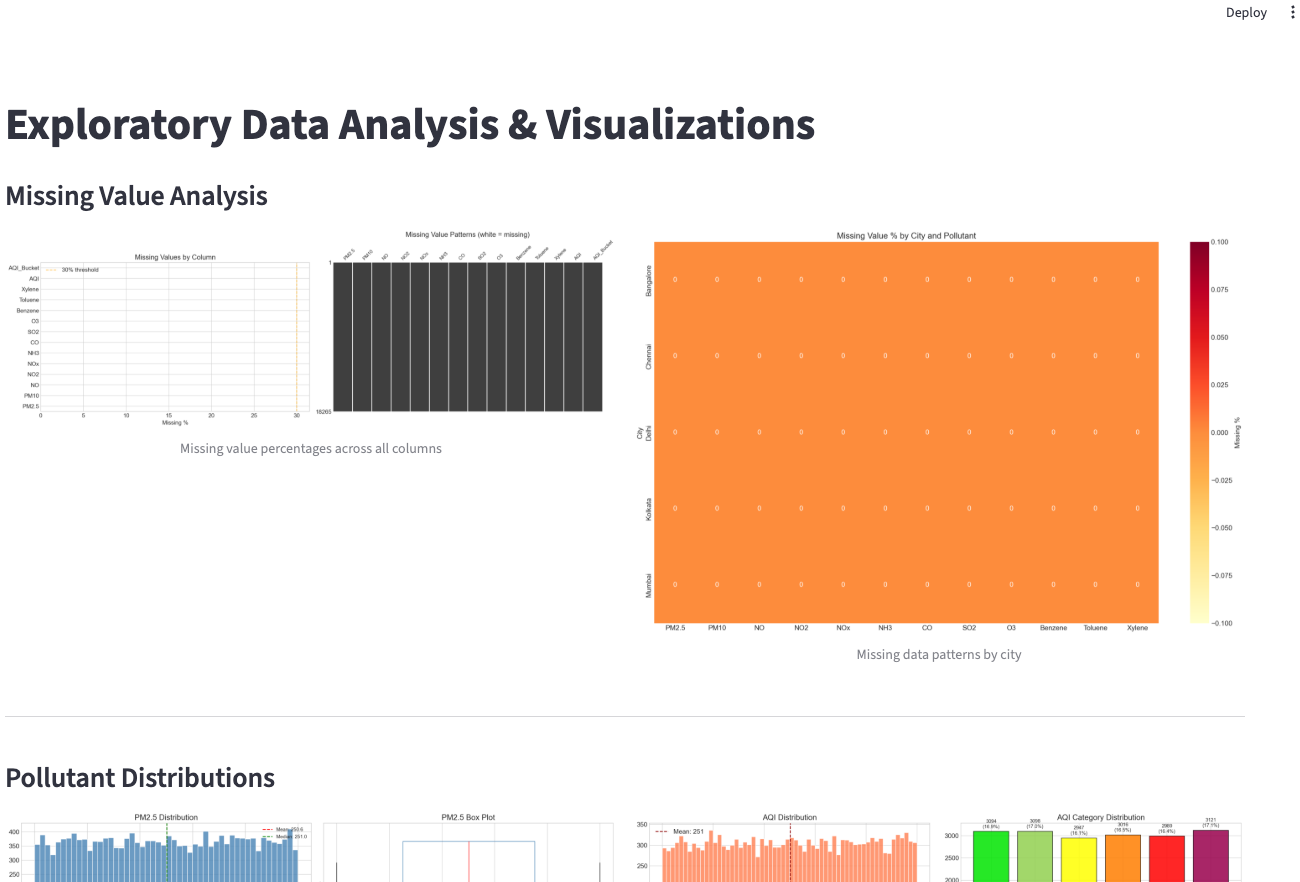
\includegraphics[width=\textwidth]{figures/ss_eda.png}
\caption{EDA Visualisations page displaying missing value analysis with per-column bar charts, missing value patterns, and per-city heatmap visualisations.}
\label{fig:ss_eda}
\end{figure}

\begin{figure}[H]
\centering
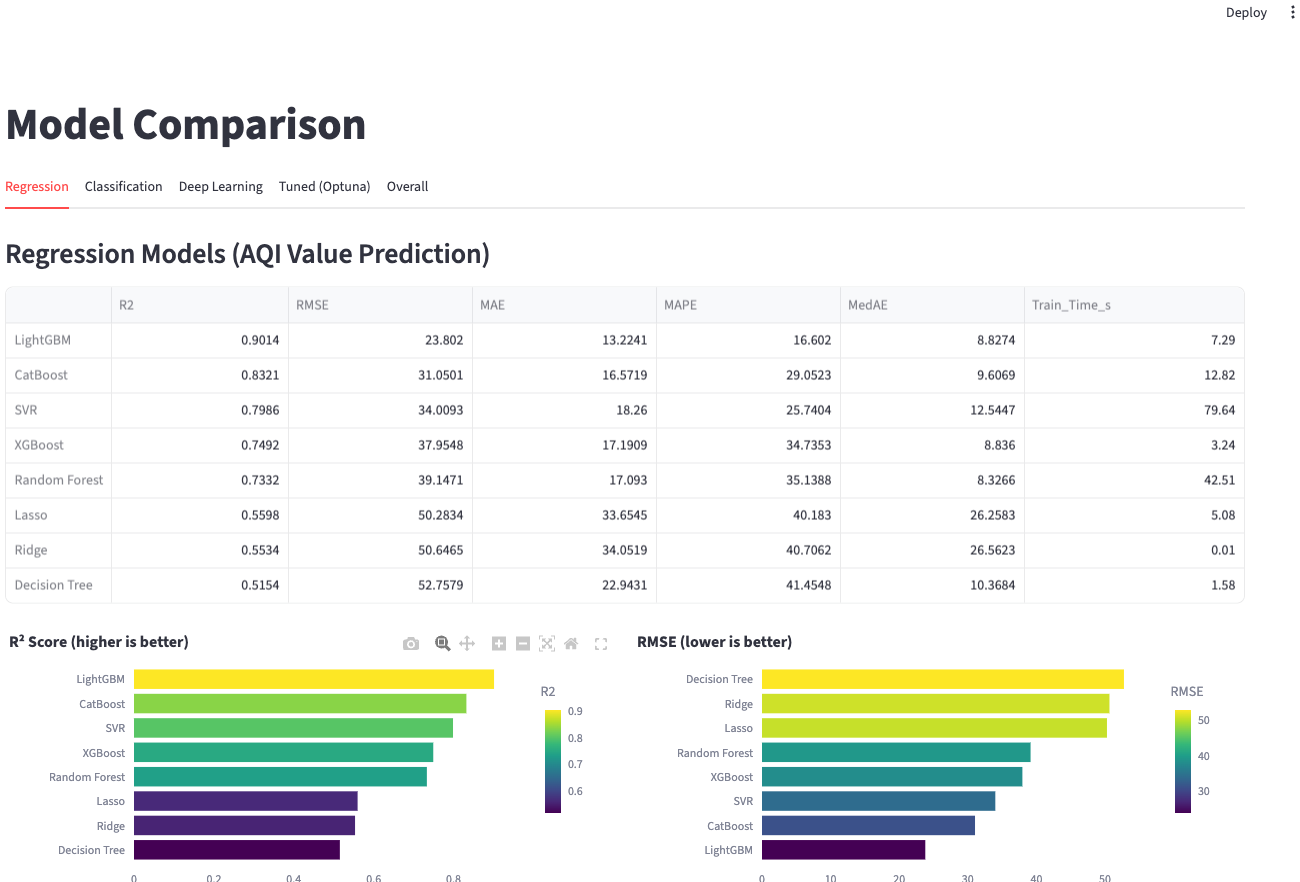
\includegraphics[width=\textwidth]{figures/ss_model_comparison.png}
\caption{Model Comparison page with tabbed interface (Regression, Classification, Deep Learning, Tuned, Overall). LightGBM achieves the best $R^2 = 0.9014$ with RMSE = 23.80 across all 8 regression models, with $R^2$ and RMSE bar charts below.}
\label{fig:ss_model_comparison}
\end{figure}

\begin{figure}[H]
\centering
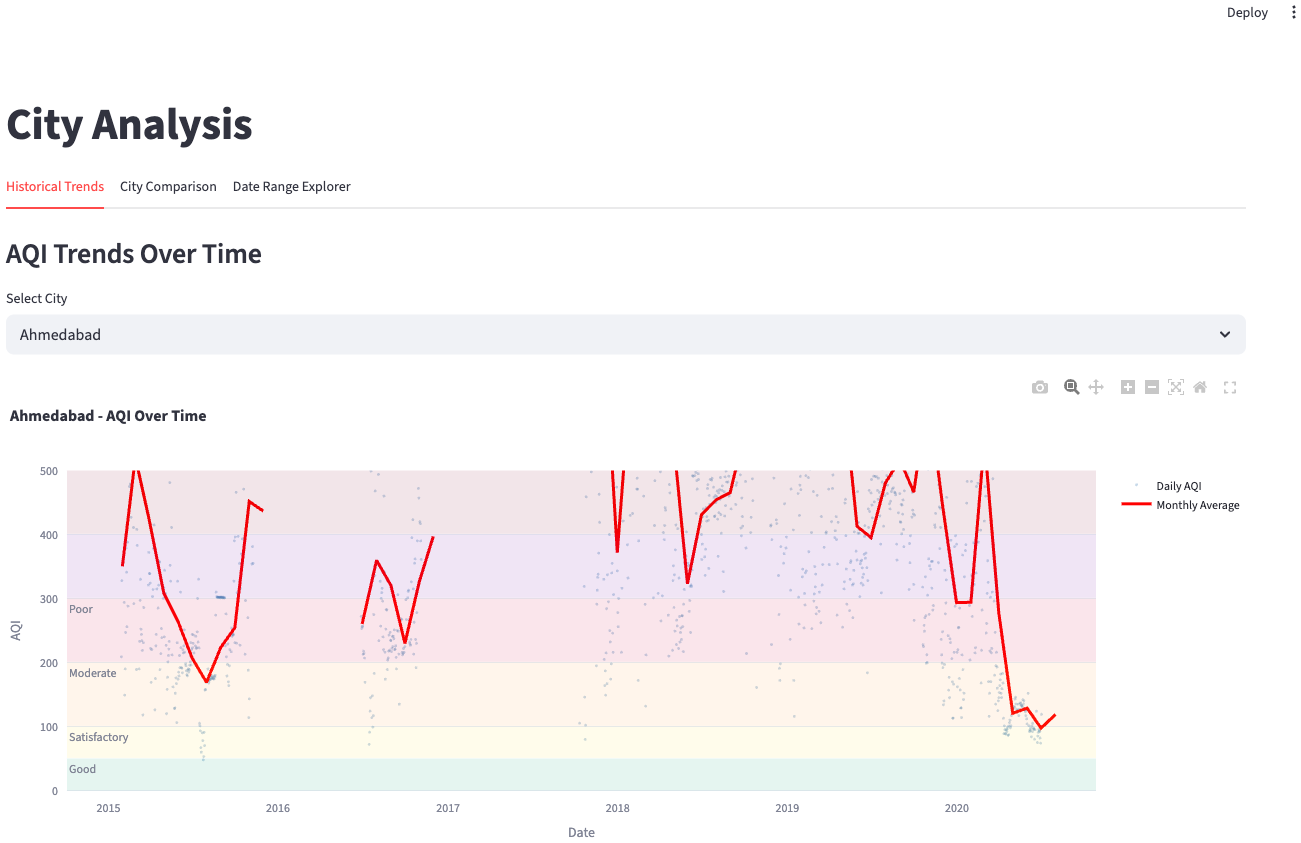
\includegraphics[width=\textwidth]{figures/ss_city_analysis.png}
\caption{City Analysis page showing historical AQI trends with daily scatter points and monthly average line for Ahmedabad (2015--2020). Colour-coded AQI severity bands (Good, Satisfactory, Moderate, Poor) provide visual context.}
\label{fig:ss_city_analysis}
\end{figure}

\section{Live Prediction System}\label{idx:s72}

The Live Prediction page (Page 5) provides two modes of operation:

\textbf{Manual Input Mode.} Users adjust pollutant concentration sliders for PM$_{2.5}$, PM$_{10}$, NO$_2$, SO$_2$, CO, O$_3$, and NH$_3$. Preset configurations are available for common scenarios: ``Delhi Winter'' (high PM$_{2.5}$/CO), ``Clean Monsoon'' (low across all), ``Moderate City'' (intermediate values). The system processes the input through both the Tuned LightGBM (Optuna, $R^2 = 0.9065$) for regression and the Tuned XGBoost (Optuna, Accuracy = 84.16\%) for classification.

\textbf{Live WAQI API Mode.} Users select from 26 Indian cities, and the system fetches real-time pollutant data from the WAQI API. Missing pollutants (notably NH$_3$, which WAQI does not provide) are filled using city-specific historical medians. The system displays three AQI values: (1) the WAQI-reported value (US-EPA scale), (2) the ML-predicted value (CPCB scale, from LightGBM), and (3) the AQI category (from XGBoost classifier).

The live prediction system implements dual AQI scales: the CPCB (Indian) scale used in training and the US-EPA scale used by international monitoring platforms. Table~\ref{tab:epa_breakpoints} presents the EPA breakpoints for PM$_{2.5}$ as an example.

\begin{table}[H]
\centering
\caption{US-EPA AQI Breakpoints for PM$_{2.5}$ (24-hour Average)}
\label{tab:epa_breakpoints}
\begin{tabular}{|l|c|c|}
\hline
\textbf{Category} & \textbf{AQI Range} & \textbf{PM$_{2.5}$ ($\mu$g/m$^3$)} \\
\hline
Good & 0--50 & 0.0--9.0 \\
\hline
Moderate & 51--100 & 9.1--35.4 \\
\hline
Unhealthy for Sensitive Groups & 101--150 & 35.5--55.4 \\
\hline
Unhealthy & 151--200 & 55.5--125.4 \\
\hline
Very Unhealthy & 201--300 & 125.5--225.4 \\
\hline
Hazardous & 301--500 & 225.5--500.4 \\
\hline
\end{tabular}
\end{table}

The system displays results through interactive AQI gauge charts that show both the WAQI Station AQI (EPA scale) and the ML Predicted AQI (CPCB scale) side by side, with colour coding matching the respective severity categories.

\begin{figure}[H]
\centering
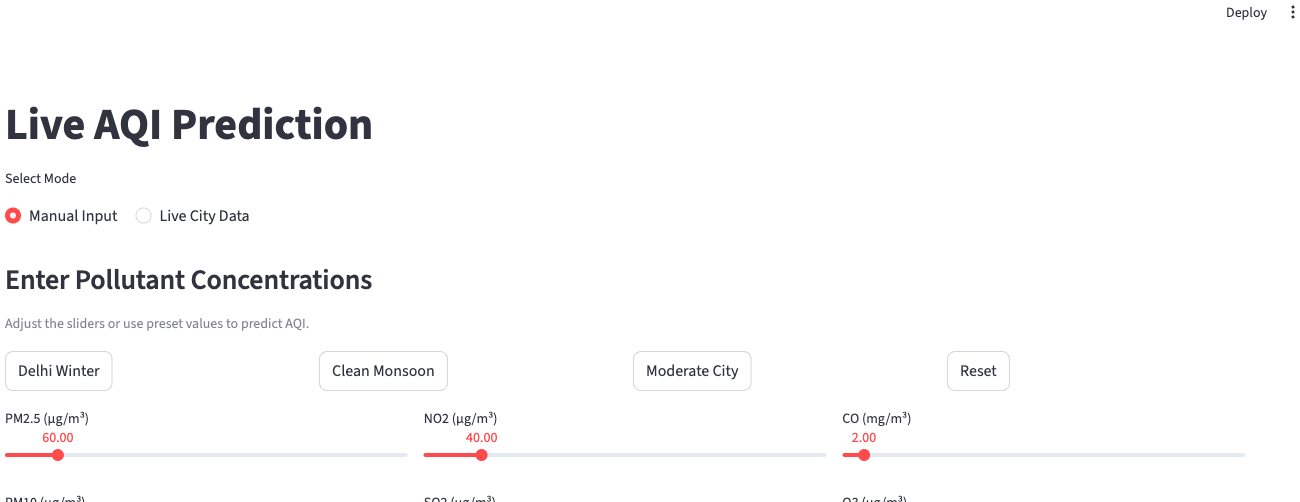
\includegraphics[width=\textwidth]{figures/ss_live_input.png}
\caption{Live Prediction page --- Manual Input mode with 7 pollutant concentration sliders (PM$_{2.5}$, PM$_{10}$, NO$_2$, SO$_2$, CO, O$_3$, NH$_3$) and preset scenario buttons (Delhi Winter, Clean Monsoon, Moderate City).}
\label{fig:ss_live_input}
\end{figure}

\begin{figure}[H]
\centering
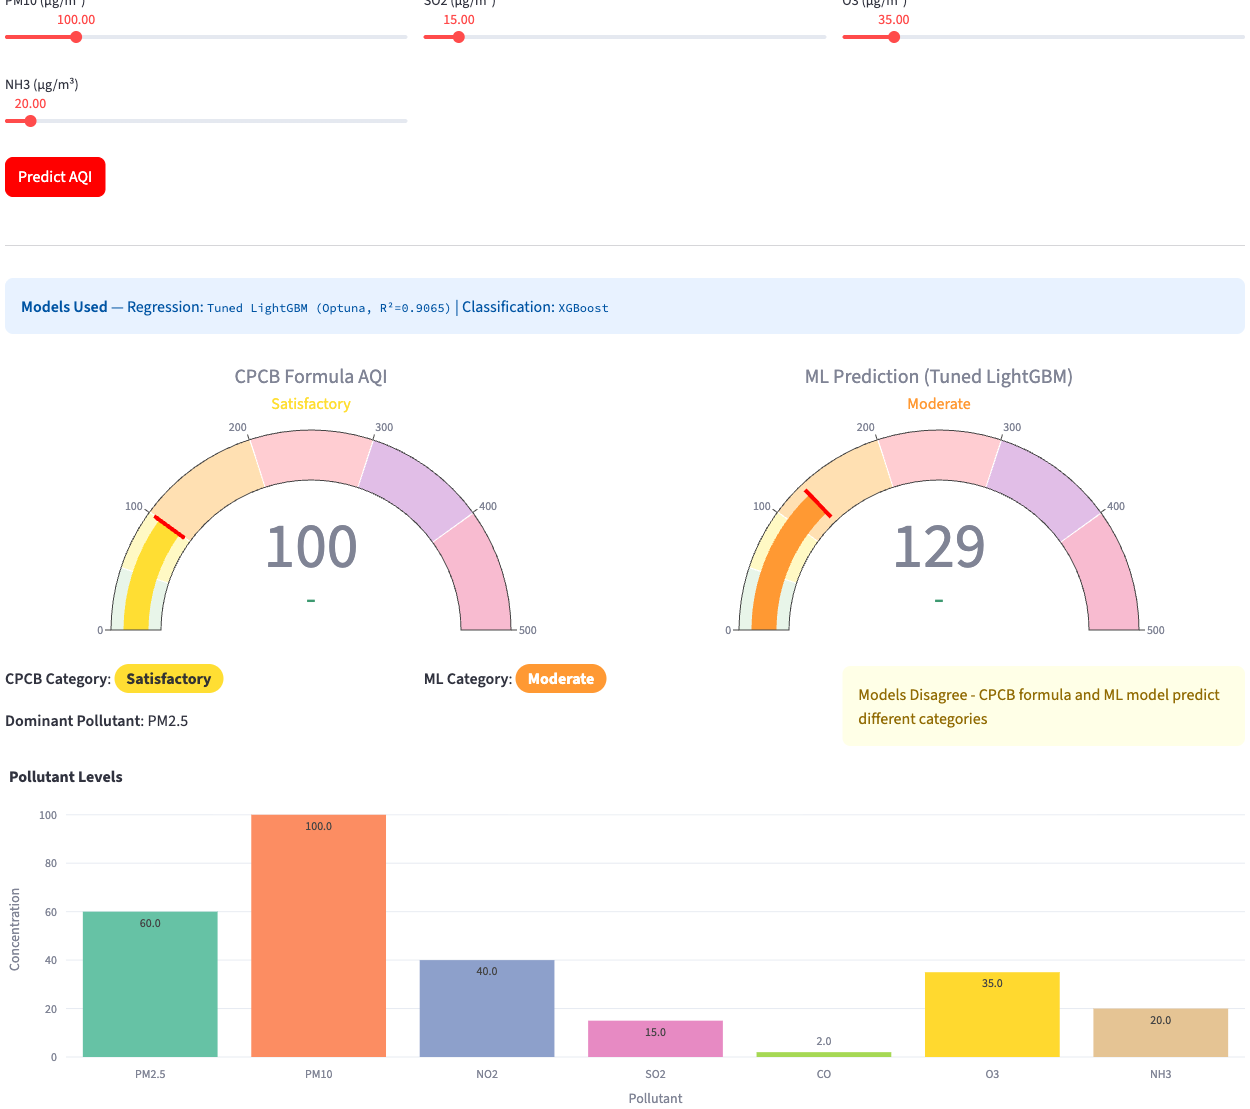
\includegraphics[width=\textwidth]{figures/ss_live_result.png}
\caption{Prediction results showing dual AQI gauge charts: CPCB Formula AQI (100, Satisfactory) and ML Prediction from Tuned LightGBM (129, Moderate). Category badges and pollutant level bar chart are displayed below.}
\label{fig:ss_live_result}
\end{figure}

\section{7-Day Forecasting Pipeline}

The forecasting module (Page 7) produces seven-day AQI forecasts by combining multiple data sources:

\textbf{Architecture.} The AQI Forecaster class integrates:
\begin{enumerate}
    \item WAQI pollutant forecasts (PM$_{2.5}$, PM$_{10}$, O$_3$ available for 3--5 day horizons)
    \item Open-Meteo weather forecasts (temperature, humidity, wind speed, precipitation)
    \item City-specific historical medians for missing pollutants
    \item Trained ML models (LightGBM regression + XGBoost classification)
\end{enumerate}

\textbf{Day-Aware Blending.} For forecast days beyond the WAQI forecast horizon, pollutant values are blended between current readings and city-specific medians using a day-aware weighting scheme: near-term forecasts (days 1--2) weight current readings at 80\%, tapering to 30\% by day 7. This captures the physical reality that current conditions are highly predictive of tomorrow but progressively less informative over longer horizons.

\textbf{Weather Adjustment Factors.} Weather conditions modulate the forecasted pollutant concentrations through physical adjustment factors:

\begin{table}[H]
\centering
\caption{Weather Adjustment Factors for AQI Forecasting}
\label{tab:weather_factors}
\begin{tabular}{|l|p{8cm}|}
\hline
\textbf{Weather Variable} & \textbf{Adjustment Logic} \\
\hline
Humidity $>$ 80\% & PM factor $\times$ 1.15 (hygroscopic growth increases measured PM) \\
\hline
Wind speed $>$ 15 km/h & PM factor $\times$ 0.80 (enhanced dispersion reduces concentrations) \\
\hline
Rainfall $>$ 5 mm & PM factor $\times$ 0.70 (wet deposition removes particulates) \\
\hline
Temperature $<$ 10$^\circ$C & Gas factor $\times$ 1.10 (inversion conditions trap gases) \\
\hline
Temperature $>$ 35$^\circ$C & O$_3$ factor $\times$ 1.15 (enhanced photochemical production) \\
\hline
\end{tabular}
\end{table}

\textbf{Forecast Smoothing.} A maximum day-to-day AQI change cap of 50\% prevents unrealistic spikes in the forecast. Each day's prediction is also anchor-blended with the previous day's prediction to produce smooth, physically plausible trajectories.

\textbf{Confidence Scoring.} Each forecast day receives a confidence score based on: (1) the forecast horizon (closer = higher confidence), (2) whether WAQI forecast data is available, and (3) the completeness of pollutant data. Day 1 forecasts typically achieve confidence scores of 80--90\%, declining to 50--60\% by day 7.

\begin{figure}[H]
\centering
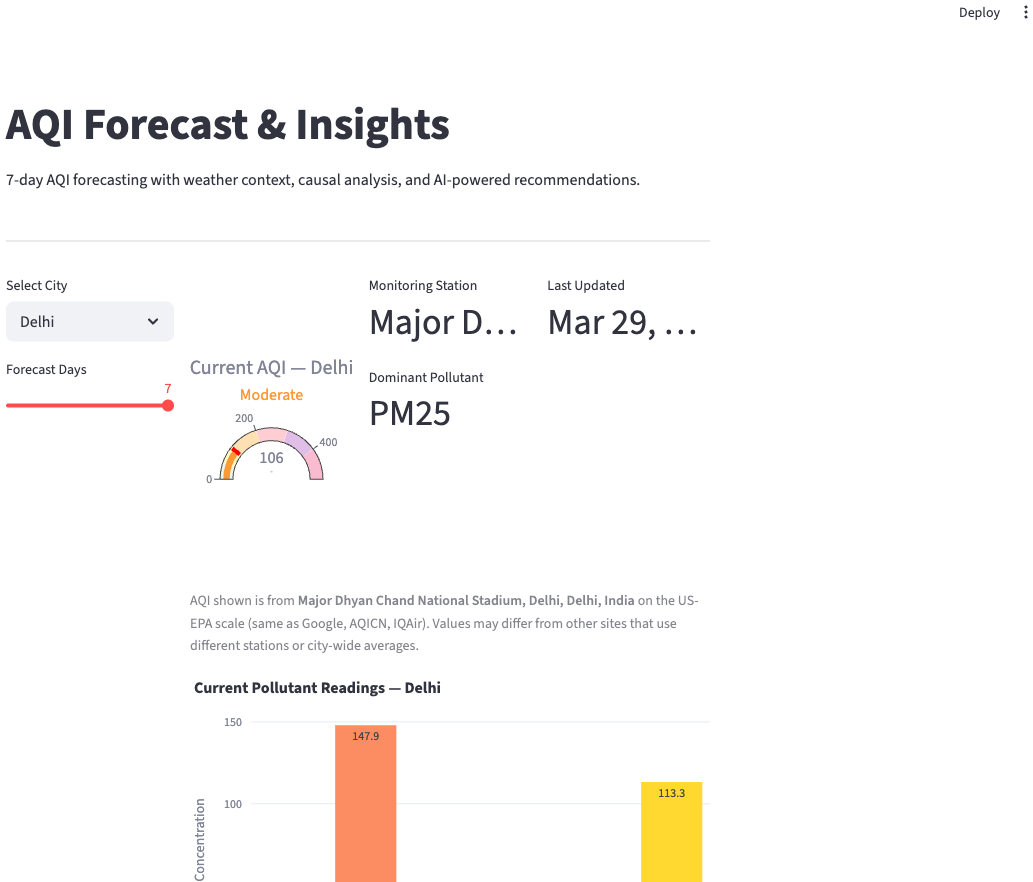
\includegraphics[width=\textwidth]{figures/ss_forecast.png}
\caption{AQI Forecast \& Insights page for Delhi showing current AQI gauge (106, Moderate), city selector, forecast day slider, monitoring station details, dominant pollutant (PM$_{2.5}$), and current pollutant readings bar chart.}
\label{fig:ss_forecast}
\end{figure}

\section{Causal Analysis Engine}

The causal analysis module identifies likely pollution sources based on pollutant concentration signatures. The system uses a rule-based approach combining pollutant signature patterns with city-specific profiles:

\textbf{Pollutant Signature Rules.} Different pollution sources produce characteristic pollutant ratios:

\begin{table}[H]
\centering
\caption{Pollutant Signature Rules for Source Identification}
\label{tab:signatures}
\small
\begin{tabular}{|l|p{5cm}|p{5cm}|}
\hline
\textbf{Source Category} & \textbf{Signature Pattern} & \textbf{Cities Affected} \\
\hline
Vehicular Emissions & High NO$_2$, elevated CO, PM$_{2.5}$/PM$_{10}$ $>$ 0.5 & Delhi, Mumbai, Bengaluru \\
\hline
Industrial Emissions & High SO$_2$, elevated CO, moderate PM & Jorapokhar, Talcher, Brajrajnagar \\
\hline
Construction Dust & High PM$_{10}$, PM$_{2.5}$/PM$_{10}$ $<$ 0.3, low gases & All cities during dry season \\
\hline
Crop Burning & Very high PM$_{2.5}$, high CO, seasonal (Oct--Nov) & Delhi, Lucknow, Patna, Chandigarh \\
\hline
Biomass Cooking & Elevated CO, moderate PM, year-round & Smaller cities, rural-adjacent \\
\hline
Photochemical Smog & High O$_3$, elevated NO$_2$, summer afternoon & All cities during summer \\
\hline
\end{tabular}
\end{table}

\textbf{City-Specific Profiles.} The system maintains profiles for 14 key cities, each with documented primary pollution sources, seasonal patterns, and geographic context. For example, Delhi's profile includes: vehicular emissions (primary), construction dust (secondary), crop burning (seasonal, Oct--Nov), and industrial emissions from surrounding NCR regions.

\textbf{Recommendations Engine.} Based on the identified pollution sources and AQI level, the system generates four categories of recommendations:
\begin{enumerate}
    \item \textbf{Health recommendations:} Activity guidance based on AQI category and vulnerable group status.
    \item \textbf{Personal protective measures:} Mask usage, air purifier guidance, outdoor activity timing.
    \item \textbf{Community actions:} Carpooling, public transport advocacy, waste management improvements.
    \item \textbf{Policy recommendations:} Emission controls, green space development, monitoring infrastructure expansion.
\end{enumerate}

\section{AI-Powered Insights}

The system integrates Google Gemini (model: gemini-2.0-flash-lite) for generating contextual, natural-language insights:

\textbf{Forecast Narrative Generation.} For each 7-day forecast, Gemini generates a narrative summary incorporating the predicted AQI trajectory, identified pollution sources, weather influences, and health implications. The prompt is engineered to produce concise, actionable insights tailored to the specific city and forecast period.

\textbf{Health Advisory Generation.} Based on the current and forecasted AQI, Gemini generates personalised health advisories for different population groups (general public, children, elderly, respiratory patients). These advisories adapt to the dominant pollutant and seasonal context.

\textbf{Template-Based Fallback.} When the Gemini API key is not configured or the API is unavailable, the system falls back to template-based insights that combine pollutant data with pre-written health guidance templates. This ensures the system remains functional without API access, though with less contextually-rich insights.

\textbf{Prompt Engineering.} The prompts provided to Gemini include: current pollutant concentrations, forecasted AQI trajectory, identified pollution sources, city profile information, seasonal context, and weather data. The system requests structured output (health advisory, activity guidance, and key findings) to ensure consistent formatting.

% %%%%%%%%%%%%%%%%%%%%%%%%%%%%%%%%%%%%%%%%%%%%%%%%%%%%%%%%%%%%
% CHAPTER 9: CONCLUSIONS
% %%%%%%%%%%%%%%%%%%%%%%%%%%%%%%%%%%%%%%%%%%%%%%%%%%%%%%%%%%%%
\clearpage
\chapter{Conclusions}\label{idx:ch8}

\section{Merits}\label{idx:s81}

This project has yielded the following key merits and achievements:

\textbf{1. Most Comprehensive Multi-Paradigm Comparison for Indian AQI.} With 20 models across three paradigms (8 regression, 7 classification, 5 deep learning), this project represents the most extensive systematic comparison for AQI prediction on Indian data, providing evidence-based model selection guidance for the environmental ML community.

\textbf{2. High Predictive Accuracy.} The Optuna-tuned LightGBM regressor achieved $R^2 = 0.9065$ with RMSE = 23.17 AQI units, explaining over 90\% of AQI variance. The XGBoost classifier attained 84.16\% accuracy with Cohen's $\kappa = 0.755$ (``substantial'' agreement). These results compare favourably with all published Indian AQI prediction studies.

\textbf{3. Feature Engineering as Primary Performance Driver.} The 141-feature engineering pipeline --- incorporating temporal lags, rolling statistics, pollutant ratios, and seasonal encodings --- was identified as the dominant determinant of predictive performance. The 35 percentage point $R^2$ improvement from linear baselines to gradient boosting quantifies the contribution of non-linear feature interactions.

\textbf{4. SHAP Validates Atmospheric Science.} The SHAP explainability analysis confirmed that the model's learned feature importance hierarchy (PM$_{2.5}$ dominance, seasonal patterns, CO combustion tracing, geographic heterogeneity) is fully consistent with established atmospheric science and the CPCB AQI methodology.

\textbf{5. COVID-19 Generalisation.} The test set's coverage of India's 2020 COVID-19 lockdown --- a period characterised by 40--60\% reductions in vehicular and industrial emissions --- demonstrated that the models generalise to unprecedented distributional shifts rather than memorising temporal trends.

\textbf{6. SMOTE Outperforms Class Weights.} Empirical comparison showed that SMOTE-based oversampling outperforms built-in class weighting by 2.7 percentage points in accuracy, providing evidence-based guidance for handling class imbalance in ordinal AQI classification.

\textbf{7. Gradient Boosting Decisively Outperforms Deep Learning.} The 23.4 percentage point $R^2$ advantage of LightGBM over the best LSTM architecture corroborates the findings of Grinsztajn et al. (2022) and contributes additional evidence to the ``tabular data'' debate in machine learning.

\textbf{8. Real-Time Deployable System.} The seven-page Streamlit dashboard demonstrates a complete pipeline from raw environmental data to deployable public health tool, with live WAQI API integration, interactive visualisations, and health advisory generation.

\textbf{9. Seven-Day Forecasting with Weather Integration.} The forecasting pipeline combines WAQI pollutant forecasts, Open-Meteo weather data, and trained ML models with day-aware blending and weather adjustment factors, producing physically plausible multi-day AQI trajectories.

\textbf{10. AI-Powered Causal Analysis and Insights.} The integration of pollutant signature analysis, city-specific profiles, and Gemini AI-powered narrative generation provides actionable insights beyond raw predictions, bridging the gap between model output and public health communication.

\section{Limitations}\label{idx:s82}

Despite the strengths enumerated above, several limitations should be acknowledged:

\textbf{1. No Meteorological Features in ML Training.} The ML models were trained exclusively on pollutant concentrations and temporal indicators. Meteorological variables (wind speed, humidity, temperature, boundary layer height) are known to significantly modulate pollutant dispersion and were not available in the CPCB dataset. Their inclusion could potentially improve regression $R^2$ by 2--5 percentage points, particularly for transitional weather conditions where pollutant concentrations alone are insufficient to predict AQI.

\textbf{2. City Treated as Categorical.} The city feature is label-encoded as an integer, which captures baseline pollution differences but does not model spatial relationships. Inter-city pollutant transport (e.g., smoke plume advection from Punjab to Delhi during crop burning season) cannot be captured by this representation.

\textbf{3. Daily Granularity Only.} The dataset operates at daily resolution, whereas hourly AQI predictions would be more useful for real-time health advisory systems. Hourly granularity would require different architectural choices (attention-based models, hourly meteorological inputs) and would face greater noise from diurnal pollution cycles.

\textbf{4. SHAP on 500 Samples.} SHAP values were computed on a stratified sample of 500 test observations for computational tractability. While this is sufficient for stable global importance rankings, individual explanations may vary slightly with larger samples, and rare feature interaction effects may be underrepresented.

\textbf{5. Single Data Source (CPCB).} The models are trained and evaluated exclusively on CPCB-verified data. External validation on independent monitoring networks (e.g., US Embassy PM$_{2.5}$ monitors, state-level pollution control boards) would strengthen generalisability claims.

\textbf{6. Live Prediction Lacks Historical Lag Context.} The live prediction system uses only current pollutant readings, whereas the trained models were optimised on a feature set that includes 72 lag features and 48 rolling statistics. This information mismatch means that live predictions may be less accurate than the reported test set metrics.

\textbf{7. Deep Learning Limited by Input.} The LSTM/GRU architectures processed only 7 raw features over 14 timesteps. With more features (meteorological data, satellite imagery), larger windows, or attention mechanisms, deep learning performance could potentially improve. The current comparison may understate deep learning's potential with richer input data.

\textbf{8. CPCB vs.\ EPA Scale Mismatch.} The WAQI API reports AQI on the US-EPA scale, while the ML models predict on the CPCB scale. Although the system computes both, the scale difference can cause confusion and the EPA-to-CPCB conversion introduces additional uncertainty.

% %%%%%%%%%%%%%%%%%%%%%%%%%%%%%%%%%%%%%%%%%%%%%%%%%%%%%%%%%%%%
% CHAPTER 10: FUTURE SCOPE & RECOMMENDATIONS
% %%%%%%%%%%%%%%%%%%%%%%%%%%%%%%%%%%%%%%%%%%%%%%%%%%%%%%%%%%%%
\clearpage
\chapter{Future Scope \& Recommendations}\label{idx:ch9}

Based on the findings and limitations of this project, the following directions are recommended for future research and development:

\textbf{1. Meteorological Feature Integration.} The most impactful improvement would be integrating meteorological variables --- wind speed and direction, temperature, relative humidity, boundary layer height, and solar radiation --- from reanalysis products (ERA5) or surface station observations. These features modulate pollutant dispersion and chemical transformation, and their inclusion is expected to improve regression $R^2$ by 2--5 percentage points, particularly for transitional weather conditions and post-monsoon crop burning events where atmospheric dynamics play a dominant role.

\textbf{2. Graph Neural Networks for Spatial Modelling.} Cities could be modelled as nodes in a geographic graph, with edges representing transport corridors (wind patterns, highway connections). Graph Neural Networks (GNNs) could capture inter-city pollutant advection --- for example, modelling how smoke from crop burning in Punjab affects AQI in Delhi, Lucknow, and Patna with a one-to-two day lag. This would replace the current city-as-categorical-variable approach with a physically grounded spatial representation.

\textbf{3. Hourly Granularity Prediction.} Extension from daily to hourly AQI prediction would support real-time health advisory systems and capture diurnal pollution cycles (morning/evening traffic peaks, afternoon ozone peaks). This requires hourly pollutant data (available from CPCB's CAAQMS stations), fundamentally different sequence modelling approaches, and careful handling of the increased noise at finer temporal resolution.

\textbf{4. Satellite-Derived PM$_{2.5}$ Integration.} NASA's MERRA-2 reanalysis and the Copernicus Atmosphere Monitoring Service (CAMS) provide global PM$_{2.5}$ estimates at 0.25$^\circ$ resolution. Incorporating satellite-derived aerosol optical depth (AOD) as a supplementary feature would provide spatial continuity beyond the 26 CPCB cities and potentially improve prediction accuracy, particularly for cities where ground monitoring data is sparse.

\textbf{5. Transfer Learning from Data-Rich to Data-Sparse Cities.} Models trained on data-rich cities (Delhi, Mumbai, Bengaluru) could be fine-tuned for data-sparse stations through domain adaptation techniques. This would extend AQI prediction capabilities to cities currently lacking sufficient historical data for standalone model training.

\textbf{6. Attention-Based Architectures.} Transformer-based architectures with self-attention mechanisms could better capture long-range temporal dependencies than LSTMs. The attention mechanism explicitly weights the importance of each past timestep, potentially improving over the fixed 14-day sliding window used in this project. With larger datasets (hourly data would provide 6$\times$ more samples), the advantage of attention mechanisms could become significant.

\textbf{7. Mobile Application Deployment.} Converting the Streamlit dashboard into a native mobile application (iOS/Android) would dramatically increase accessibility, particularly for the general public. Push notifications for AQI alerts, location-based predictions, and personalised health advisories based on user health profiles would enhance the public health impact.

\textbf{8. Integration with Government Alert Systems.} The forecasting pipeline could be integrated with Delhi's Graded Response Action Plan (GRAP) and similar state-level alert systems, providing automated early warning when AQI is forecast to exceed threshold levels. This would reduce the response lag between forecast and intervention.

\textbf{9. Multi-Pollutant Interaction Modelling.} The current feature engineering captures some pollutant interactions (PM$_{2.5}$/PM$_{10}$ ratio, NO$_2$/NO ratio), but explicit modelling of photochemical interaction cycles (NO$_x$-O$_3$ titration, secondary organic aerosol formation) through domain-knowledge-informed feature engineering or physics-guided neural networks could improve predictions for ozone and secondary PM$_{2.5}$.

\textbf{10. Extended Time Series (2015--2025).} Incorporating more recent data (2021--2025) would capture post-COVID pollution recovery trends, the impact of BS-VI emission norms (implemented April 2020), and the expansion of electric vehicle adoption. A longer time series would also strengthen the training of deep learning models, potentially narrowing the gap with gradient boosting methods.

% %%%%%%%%%%%%%%%%%%%%%%%%%%%%%%%%%%%%%%%%%%%%%%%%%%%%%%%%%%%%
% CHAPTER 11: REFERENCES
% %%%%%%%%%%%%%%%%%%%%%%%%%%%%%%%%%%%%%%%%%%%%%%%%%%%%%%%%%%%%
\clearpage
\chapter{References}\label{idx:ch10}

\begin{enumerate}[leftmargin=1.5cm, label={[\arabic*]}]

\item World Health Organization, ``WHO Global Air Quality Guidelines: Particulate Matter (PM$_{2.5}$ and PM$_{10}$), Ozone, Nitrogen Dioxide, Sulfur Dioxide and Carbon Monoxide,'' WHO, Geneva, 2021.

\item K.~Balakrishnan \textit{et al.}, ``The impact of air pollution on deaths, disease burden, and life expectancy across the states of India: the Global Burden of Disease Study 2017,'' \textit{The Lancet Planetary Health}, vol.~3, no.~1, pp.~e26--e39, 2019.

\item S.~K. Guttikunda and R.~Calori, ``A GIS based emissions inventory at 1~km $\times$ 1~km spatial resolution for air pollution analysis in Delhi, India,'' \textit{Atmospheric Environment}, vol.~67, pp.~101--111, 2013.

\item Central Pollution Control Board (CPCB), ``National Air Quality Index,'' Ministry of Environment, Forest and Climate Change, Government of India, 2014.

\item K.~Kumar and B.~P. Pande, ``Air pollution prediction with machine learning: a case study of Indian cities,'' \textit{International Journal of Environmental Science and Technology}, vol.~20, pp.~5333--5348, 2023.

\item E.~Sharma, R.~Deo, R.~Prasad, and A.~V. Parisi, ``A hybrid air quality early-warning framework: an hourly forecasting model with online sequential extreme learning machines and empirical mode decomposition algorithms,'' \textit{Science of the Total Environment}, vol.~709, p.~135934, 2020.

\item A.~Masood and K.~Ahmad, ``A review on emerging artificial intelligence (AI) techniques for air pollution forecasting: fundamentals, application and performance,'' \textit{Journal of Cleaner Production}, vol.~322, p.~129072, 2021.

\item L.~Grinsztajn, E.~Oyallon, and G.~Varoquaux, ``Why do tree-based models still outperform deep learning on typical tabular data?,'' in \textit{Proc. NeurIPS 2022 Datasets and Benchmarks Track}, 2022.

\item S.~Mahato, S.~Pal, and K.~G. Ghosh, ``Effect of lockdown amid COVID-19 pandemic on air quality of the megacity Delhi, India,'' \textit{Science of the Total Environment}, vol.~730, p.~139086, 2020.

\item T.~Chen and C.~Guestrin, ``XGBoost: A scalable tree boosting system,'' in \textit{Proc. 22nd ACM SIGKDD Int. Conf. Knowledge Discovery and Data Mining}, pp.~785--794, 2016.

\item G.~Ke \textit{et al.}, ``LightGBM: A highly efficient gradient boosting decision tree,'' in \textit{Advances in Neural Information Processing Systems}, vol.~30, pp.~3146--3154, 2017.

\item L.~Prokhorenkova, G.~Gusev, A.~Vorobev, A.~V. Dorogush, and A.~Gulin, ``CatBoost: unbiased boosting with categorical features,'' in \textit{Advances in Neural Information Processing Systems}, vol.~31, 2018.

\item S.~Hochreiter and J.~Schmidhuber, ``Long Short-Term Memory,'' \textit{Neural Computation}, vol.~9, no.~8, pp.~1735--1780, 1997.

\item K.~Cho \textit{et al.}, ``Learning phrase representations using RNN encoder-decoder for statistical machine translation,'' in \textit{Proc. EMNLP}, pp.~1724--1734, 2014.

\item L.~Breiman, ``Random Forests,'' \textit{Machine Learning}, vol.~45, no.~1, pp.~5--32, 2001.

\item C.~Cortes and V.~Vapnik, ``Support-vector networks,'' \textit{Machine Learning}, vol.~20, no.~3, pp.~273--297, 1995.

\item S.~M. Lundberg and S.-I. Lee, ``A unified approach to interpreting model predictions,'' in \textit{Advances in Neural Information Processing Systems}, vol.~30, pp.~4765--4774, 2017.

\item M.~T. Ribeiro, S.~Singh, and C.~Guestrin, ```Why should I trust you?': Explaining the predictions of any classifier,'' in \textit{Proc. 22nd ACM SIGKDD}, pp.~1135--1144, 2016.

\item S.~M. Lundberg \textit{et al.}, ``From local explanations to global understanding with explainable AI for trees,'' \textit{Nature Machine Intelligence}, vol.~2, pp.~56--67, 2020.

\item C.~Molnar, \textit{Interpretable Machine Learning: A Guide for Making Black Box Models Explainable}, 2nd~ed., 2022.

\item N.~V. Chawla, K.~W. Bowyer, L.~O. Hall, and W.~P. Kegelmeyer, ``SMOTE: Synthetic Minority Over-sampling Technique,'' \textit{Journal of Artificial Intelligence Research}, vol.~16, pp.~321--357, 2002.

\item O.~Troyanskaya \textit{et al.}, ``Missing value estimation methods for DNA microarrays,'' \textit{Bioinformatics}, vol.~17, no.~6, pp.~520--525, 2001.

\item T.~Akiba, S.~Sano, T.~Yanase, T.~Ohta, and M.~Koyama, ``Optuna: A next-generation hyperparameter optimization framework,'' in \textit{Proc. 25th ACM SIGKDD}, pp.~2623--2631, 2019.

\item R.~Shwartz-Ziv and A.~Armon, ``Tabular data: Deep learning is not all you need,'' \textit{Information Fusion}, vol.~81, pp.~84--90, 2022.

\item V.~Borisov \textit{et al.}, ``Deep neural networks and tabular data: A survey,'' \textit{IEEE Transactions on Neural Networks and Learning Systems}, vol.~35, no.~6, pp.~7499--7519, 2024.

\item X.~Li, L.~Peng, X.~Yao, S.~Cui, Y.~Hu, C.~You, and T.~Chi, ``Long short-term memory neural network for air pollutant concentration predictions: method development and evaluation,'' \textit{Environmental Pollution}, vol.~231, pp.~997--1004, 2017.

\item U.~Pak, J.~Ma, U.~Ryu, K.~Ryom, U.~Juhyok, K.~Pak, and C.~Pak, ``Deep learning-based PM2.5 prediction considering the spatiotemporal correlations: a case study of Beijing, China,'' \textit{Science of the Total Environment}, vol.~699, p.~134279, 2020.

\item M.~Castelli, F.~M. Clemente, A.~Popovic, S.~Silva, and L.~Vanneschi, ``A machine learning approach to predict air quality in California,'' \textit{Complexity}, vol.~2020, p.~8049504, 2020.

\item P.~W. Soh, J.~W. Chang, and J.~N. Huang, ``Adaptive deep learning-based air quality prediction model using the most relevant spatial-temporal relations,'' \textit{IEEE Access}, vol.~6, pp.~58186--58199, 2018.

\item S.~Sharma, M.~Zhang, Anshika, J.~Gao, H.~Zhang, and S.~H. Kota, ``Effect of restricted emissions during COVID-19 on air quality in India,'' \textit{Science of the Total Environment}, vol.~728, p.~138878, 2020.

\item J.~D. Berman and K.~Ebisu, ``Changes in US air quality during the COVID-19 pandemic,'' \textit{Science of the Total Environment}, vol.~739, p.~139864, 2020.

\item T.~Ganguly \textit{et al.}, ``National Clean Air Programme (NCAP) for Indian Cities: Review and outlook of clean air action plans,'' \textit{Atmospheric Environment: X}, vol.~8, p.~100096, 2020.

\item T.~Hastie, R.~Tibshirani, and J.~Friedman, \textit{The Elements of Statistical Learning}, 2nd~ed., Springer, 2009.

\item Ministry of Environment, Forest and Climate Change, ``National Clean Air Programme (NCAP),'' Government of India, 2019.

\end{enumerate}

% ============================================================
% END DOCUMENT
% ============================================================
\end{document}
